%
% Modified by Megan Patnott
% Last Change: Jan 18, 2013
%
%%%%%%%%%%%%%%%%%%%%%%%%%%%%%%%%%%%%%%%%%%%%%%%%%%%%%%%%%%%%%%%%%%%%%%%%
%
% Modified version of the sample_ndthesis.tex
% by Sameer Vijay
% Last Change: Wed Jul 27 2005 14:00 CEST
%
%%%%%%%%%%%%%%%%%%%%%%%%%%%%%%%%%%%%%%%%%%%%%%%%%%%%%%%%%%%%%%%%%%%%%%%%
%
% Sample Notre Dame Thesis/Dissertation
% Using Donald Peterson's ndthesis classfile
%
% Written by Jeff Squyres and Don Peterson
%
% Provided by the Information Technology Committee of
%   the Graduate Student Union
%   http://www.gsu.nd.edu/
%
% Nothing in this document is serious except the format.  :-)
%
%%%%%%%%%%%%%%%%%%%%%%%%%%%%%%%%%%%%%%%%%%%%%%%%%%%%%%%%%%%%%%%%%%%%%%%%
% This is *not* a substitute for the documentation, which is included
% as a pdf file in the standard distribution, and can be obatined from
% the dtx file in the advanced distribution.
%%%%%%%%%%%%%%%%%%%%%%%%%%%%%%%%%%%%%%%%%%%%%%%%%%%%%%%%%%%%%%%%%%%%%%%%
%
% You should *also* have a ND formatting guide to ensure that you have
% all the relevant parts, put the captions in the right place, etc.
% Just because you have this wonderful style classfile doesn't mean
% that it removes *all* the formatting onus from you.  :-)
% Although be warned that the Graduate School has been known to let
% their official formatting guide get out of date. When in doubt,
% the Microsoft Word example seemed to be the only thing kept
% consistently up-to-date in 2013, and is probably the safest thing
% to consult.
%
% You should break all of this stuff up into separate files
% (at the very least, one chapter per file) and use the \include
% command, as has been done here for chapters 1 and 2 and the appendix.
% There is also an \input command, but \include is more commonly used to
% import chapters in books and dissertations. For the differences between these
% two commands, see, e.g., 
% http://web.science.mq.edu.au/~rdale/resources/writingnotes/latexstruct.html
% or http://tex.stackexchange.com/questions/246/when-should-i-use-input-vs-include.
%
% If you compile from the command line, note that you should also have 
% a good Makefile; one that invokes LaTeX as many times as necessary 
% (up to 4) and bibtex if necessary.
%
% If you use an editor that allows you to compile from within the
% program, note that you will need to compile up to four times. Also,
% we recommend that you use pdflatex (sometimes displayed as
% LaTeX => PDF) to compile directly to pdf.
%
% If you have any suggestions, comments, questions, please send e-mail
% to: dteditor@nd.edu
%
%%%%%%%%%%%%%%%%%%%%%%%%%%%%%%%%%%%%%%%%%%%%%%%%%%%%%%%%%%%%%%%%%%%%%%%%

\documentclass[final,numrefs,sort&compress,noinfo, twoadvisors]{nddiss2e}
% One of the options draft, review, final must be chosen.
% One of the options textrefs or numrefs should be chosen
% to specify if you want numerical or ``author-date''
% style citations.
% Other available options are:
% 10pt/11pt/12pt (available with draft only)
% twoadvisors
% noinfo (should be used when you compile the final time
%         for formal submission)
% sort (sorts multiple citations in the order that they're
%       listed in the bibliography)
% compress (compresses numerical citations, e.g. [1,2,3]
%           becomes [1-3]; has no effect when used with
%           the textrefs option)
% sort&compress (sorts and compresses numerical citations;
%           is identical to sort when used with textrefs)
\usepackage{braket}
\usepackage{multirow}

\begin{document}

\frontmatter % All the items before the first chapter go in ``frontmatter''

% Your title must be in all caps, and you must do this manually!
% Titles may be 1-4 lines long. If your title is longer than 4 lines, the class file
% may have difficulty formatting the title page.
\title{DEVELOPMENT AND APPLICATIONS OF REAL-SPACE ELECTROSTATIC INTERACTION METHODS FOR CHARGE-MULTIPOLES IN CONDENSED PHASE ENVIRONMENTS}
\author{Madan Lamichhane}
\work{Dissertation} % or \work{Thesis}
\degaward{Doctor of Philosophy} % or 
%\degaward{Master of Science \\ in \\ Subject}
\advisor{Kathie E. Newman}
\secondadvisor{J. Daniel Gezelter} % if you have two advisers are using the option twoadvisors
\department{Physics}

\maketitle
%%%%%%%%%%%%%%%%%%%%%%%%%%%%%%%%%%%%%%%%%%%%%%%%%%%%%%%%%%%%%%%%%%%%%%%%
%
% Front stuff
%
%%%%%%%%%%%%%%%%%%%%%%%%%%%%%%%%%%%%%%%%%%%%%%%%%%%%%%%%%%%%%%%%%%%%%%%%

% You must either set the copyright information or put your work in the public domain.
%\copyrightholder{Madan Lamichhane} % See template or documentation for
%\copyrightyear{2016}           % other copyright options.
%\makecopyright

% An abstract is optional for a mster's thesis, and required for a doctoral dissertation.
\begin{abstract}
Computing electrostatic interaction is the most expensive portion of a  molecular simulation. Generally, traditional and modified Ewald methods are well known for calculating electrostatic interaction in molecular dynamics (MD) communities. But these methods are computationally very expensive for larger system. Nowadays there is a growing interest in developing real space method, scales linearly with the system size. The real space method for the charge-charge interaction was originally developed by \textit{Wolf} and extended by \textit{Gezelter et al.}. In this dissertation, I present three new real-space methods: Shifted Potential (SP), Gradient-Shifted Force (GSF), and Taylor-Shifted Force (TSF), for computing electrostatic interaction between dipoles and quadrupoles. I also discuss the various static and dynamic properties evaluated using newly developed real space methods.  Additionally, I present three methods: fluctuation, perturbation, and potential of mean force (PMF) methods, for computing dielectric properties for multipolar fluids. 

The SP method is the multipolar version of the \textit{Wolf}'s electrostatic method. Similarly, the GSF and TSF method are natural extension of original Damped Shifted Force (DSF) method developed by  \textit{Fennell} and \textit{Gezelter}. The energies evaluated using SP method shows quantitative agreement with Ewald sum, therefore good choice for monte carlo (MC) simulation. The energies, forces, and torques calculated from the GSF method agrees with the Ewald's result and produce excellent conservation of energy in MD simulations. Both SP and GSF method with suitable damping parameter performs remarkably well in predicting static and dynamic properties of the liquid systems. 

For the both dipolar and quadrupolar fluids, the dielectric properties predicted using perturbation method agree with fluctuation formula. We need a correction factor to obtain the dielectric constant and susceptibility from the directly measurable polarizability from the simulation. I tabulate the correction factors for both dipolar and quadrupolar fluid for all real-space as well as Ewald method. Finally, the dielectric screening from the perturbation and fluctuation method are compared with directly measured screening factor using PMF method.  
\end{abstract}

% A dedication is optional.
%\renewcommand{\dedicationname}{DEDICATION}
\begin{dedication}
  To my late father Hari Bahadur Lamichhane and mother Dropati Lamichhane for their hard work, consistent support, love, and inspiration. 
\end{dedication}

% These are required, and must be in this order.
\tableofcontents
\listoffigures
\listoftables

% A preface is optional.
%\begin{preface}
%  I would like to preface this work with all the wonderful things that
%  Gnus have brought to our society: trees, dirt, flowers, grass,
%  lakes, and other earthly-things.  We should not forget them in our
%  daily lives.
%
%  Additionally, we should offer them food for all their hard work.  In
%  fact, Gnus work so hard that they sleep for the colder half of
%  the year.  As such, they tend to grow a little rotund.  Humans
%  should not fault them for this, as it is necessary for their
%  survival.  Indeed, many humans grow rotund on their on accord!
%\end{preface}

% It's hard to tell from the information available from the Graduate
% School in Spring 2013 whether or not an acknowledgements section is optional.
\begin{acknowledge}
First of all, I would like to express my deepest appreciations to my advisors, Professor Kathie E. Newman and Professor J. Dainel Gezelter for their persistent guidance, support, and inspiration. Without their help this dissertation would not have been possible.

I am grateful to my dissertation committee; Professor Morten Eskildsen, Professor Mark Alber, and Professor Rebecca Surman, for their valuable time, support, and suggestions. I am also thankful my research group: Dr. Joseph Michalka, Patrick Louden, Suzanne Kucera, Hemanta Bhattarai, Dr. Kelsey Stocker, and Thomas Parsons for their help, support, and valuable discussion.

I am very grateful to my wife Sumitra for her unconditional love, support, inspiration, and great patience throughout the course of my PhD research.  Without her, completing research would not this easy for me. I am also very thankful to my Parents: Hari B. Lamichhane and Dropati Lamichhane,  Brothers: Bishal and Prabin, and  Sisters: Indira and Rekha. My family has always been great source of inspiration for me. Without their support and encouragement, I would not have achieved this opportunity. I am indebted to my friends: Aboutaleb Amiri and Melinda Varga for their valuable support and discussion.

Financial support for this research was provided by the National Science Foundation (NSF) under grant CHE-1362211 and computational time was provided by the Center for Research Computing (CRC) at the University of Notre Dame.
\end{acknowledge}

\mainmatter
% Place the text body here.
%\include{chapter-one}
%Begin each chapter with \chapter{TITLE}. Chapter titles must be in all caps
%and ensuring that they are is your responsibility.

%
% Chapter 1
%

%
% Modified by Megan Patnott
% Last Change: Jan 18, 2013
%
%%%%%%%%%%%%%%%%%%%%%%%%%%%%%%%%%%%%%%%%%%%%%%%%%%%%%%%%%%%%%%%%%%%%%%%%
%
% Modified by Sameer Vijay
% Last Change: Tue Jul 26 2005 13:00 CEST
%
%%%%%%%%%%%%%%%%%%%%%%%%%%%%%%%%%%%%%%%%%%%%%%%%%%%%%%%%%%%%%%%%%%%%%%%%
%
% Sample Notre Dame Thesis/Dissertation
% Using Donald Peterson's ndthesis classfile
%
% Written by Jeff Squyres and Don Peterson
%
% Provided by the Information Technology Committee of
%   the Graduate Student Union
%   http://www.gsu.nd.edu/
%
% Nothing in this document is serious except the format.  :-)
%
% If you have any suggestions, comments, questions, please send e-mail
% to: ndthesis@gsu.nd.edu
%
%%%%%%%%%%%%%%%%%%%%%%%%%%%%%%%%%%%%%%%%%%%%%%%%%%%%%%%%%%%%%%%%%%%%%%%%
%
% Chapter 1
%

%\documentclass{article}
%\usepackage{mathtools}

\chapter{INTRODUCTION}

In computer simulation of condensed phase molecular systems, molecules are commonly represented by atomic sites that interact by a parametrized forcefield. This forcefield aims to reproduce observable phenomena, by incorporating the proper physics into the simulation. There are mainly two types of interaction; intramolecular and intermolecular, which determines the static and dynamic properties of the molecular systems. Intramolecular interaction is the interaction within a single molecules which includes, bonding, bending, torsion etc whereas intermolecular interaction is the interaction between two or more molecules which includes van der Waals and electrostatic interactions due to full or partial charges located on or near the atomic sites. The computation of these electrostatic interactions is the most expensive portion of a molecular simulations. Due to this, there have been significant efforts to develop practical, efficient, and accurate methods for evaluating electrostatic interactions. 

The Ewald method is one of the most well known and accurate method but it is computationally expensive scaling as O($N^2$), where $N$ is the total number of particles. The appropriate selection of damping paramenter and suitable algorithm can decrease computational cost to O($N^{3/2}$)\cite{Perram88}. Modification of the Ewald method, including a particle mesh and fast Fourier transform (FFT) have decreased its cost down to O($N\log N$) \cite{Shimada93, Luty95, Darden93,Essmann95}. But these modified Ewald methods (particle mesh Ewald (PME), particle-particle particle-mesh Ewald (P3ME)) are still computationally expensive. In addition to this, the Ewald method requires an inherent periodicity which can be problematic in a number of protein/solvent and ionic solution environments \cite{Roberts94,Roberts95,Luty96,Hunenberger99a,Hunenberger99b,Weber00,Gezelter06}. To address these problems a lot of interest is currently growing in developing efficient real space electrostatic methods which scales linearly with the system size i.e. O($N$). This method was originally proposed by wolf \textit{et al.} \cite{Wolf99} and extended initially by Zahn \textit{et al.}\cite{Zahn02} then by C.J. Fennell and J. D. Gezelter \cite{Gezelter06}. All these methods were limited to charge-charge interactions between atomic cites. Our research developed real-space electrostatic interaction methods for higher order charge-multipoles (dipoles and quadrupoles) and studied their applications and performance in various condensed phase environments. This research also studied various static, dynamic, and dielectric properties for molecular systems using newly developed real space methods. 

%which the conditionally convergent sum of the electrostatic energy is converted into two absolutely convergent terms, one being evaluated in real space and the other in reciprocal space \cite{ Allen87, deLeeuw80, Ewald21,Smith81}. Calculation of the reciprocal term is very inefficient which makes
%
%Often this includes a Lennard-Jones potential and electrostatic interactions due to full or partial charges located on or near the atomic sites. 

This dissertation consists of five chapters. First chapter is an introductory chapter initially outlines the background and motivation of the research. It also briefly  discusses the basic principles of widely used molecular simulation methods: Molecular Dynamics (MD) and Monte Carlo (MC) simulations, where the newly developed electrostatic methods are very useful. Similarly this chapter also describes traditional Ewald as well as various improved Ewald based methods: P3ME, PME, and Multiple-based Ewald. Additionally it presents the problems caused due to the spherical truncation in real-space methods and discusses various technique implemented to resolve this problem in the past.

Chapter 2 presents the mathematical formulation of our newly developed real-space electrostatic methods: Gradient-shifted Force (GSF), Shifted-potential (SP), and Taylor-shifted force (TSF). It also compares energy constant evaluated  using newly developed methods with analytical results for different types dipolar and quadrupolar crystals.

The accuracy newly developed methods have been tested against Ewald in Chapter 3. Furthermore various static and dynamic properties evaluated from real space methods are also compared with traditional Ewald method. The test of total energy conservation is very important in MD simulations which is also studied in this chapter. 

Chapter 4 describes three different ways of evaluating the dielectric properties for dipolar and quadrupolar liquids using Flcutuation, Perturbation, and Potential of Mean Force (PMF) methods. This chapter also explores the correction factor required to obtain correct dielectric using  GSF, SP, and TSF methods. In addition, the dielectric properties; susceptiblity and dielectric constant, obtained using all three different methods are compared with each other as well as with previous simulation result in case of Stockmayer fluid.

Finally Chapter 5 summarizes, draw conclusion and discusses future directions, applications, and limitations of my research. 

\section{Molecular Dynamics (MD) Simulation}

Molecular dynamics is computer simulation method for studying static and dynamic properties for molecular systems. In this method, each atom or molecule interacts with other molecules in the system and evolve dynamically following classical equation of motion. The numerical step-by-step process for MD is outlined in Figure \ref{fig:MD}. 
    
\begin{figure}[tpb]
  \begin{center}
    \centerline{\includegraphics[scale=0.8]{MD_flowchart.pdf}}
    \caption{Schematic figure showing step-by-step process in Molecular dynamics simulation algorithm.}
    \label{fig:MD}
  \end{center}
\end{figure}

In MD simulation, first of all molecules are initialized by assigning their initial positions and velocities at given boundary conditions. Molecules are usually initialized in such a way so that system does not take very long time to reach equilibrium. Before moving a molecule in the system, we need to evaluate its potential energy which is mainly due to intramolecular interactions within the molecule itself as well as intermolecular interactions with all other molecules in the system. We can write the potential energy for a molecule in a system as shown in below:
\begin{equation}
U(\mathbf r) = \overbrace{U_{bond} + U_{bend} + U_{torsion}}^{Intramolecular\; interactions} + \overbrace{U_{electrostatic} + U_{van\;der \;Waals}}^{Intermolecular\;interactions} + ...
\label{eq:potential}
\end{equation}   
In equation \ref{eq:potential} the energy due to bonding, bending, and torsion represents intramolecular interactions whereas electrostatic and van der Waals represents intermolecular interactions. The force and torque acting on the molecule is obtained using following equations.

\begin{subequations}
\begin{gather}
\mathbf F (\mathbf r) = \nabla_r U(\mathbf r) \\
\mathbf {\mathbf{T}}(\mathbf r) = \mathbf r \times \nabla_r U(\mathbf r).
\end{gather}
\label{eq:forceTorque}
\end{subequations}

The force and torque provides the required dynamics to the molecule at a given time step. The same process is repeated for every molecules in the system. Once the molecules move forward by time step following prescribed equation of motion, their positions and velocities are adjusted according to applied boundary conditions (i.e temperature, pressure, volume etc) in the system. After adjusting positions and velocities, again we can evaluate the potential energy for each molecule and repeat same process till the simulation completes its predetermined simulation time.
 
In MD simulations, the intermolecular interactions are most expensive parts of simulation. Among them van der Waals interaction is short range interaction usually described by Lennard-Jones (LJ) potential can be written as,

\begin{equation}
U_{LJ}(r) = 4\epsilon \left[\left(\frac{\sigma}{r} \right)^{12} - \left(\frac{\sigma}{r} \right)^6\right],
\label{eq:LJ}
\end{equation}
where $\sigma$ is diameter of a molecule and $\epsilon$ determines well depth of the attractive potential. Above equation \ref{eq:LJ} clearly shows it decays much faster with the distance therefore considered as short-range interaction. The repulsive part of the  LJ potential $ \textit{~}\frac{1}{r^{12}}$ prevents two or more molecules to occupy same position. The electrostatic interactions are considered as long-range interaction. If we consider charge-charge interactions between molecules then they interact with Coulomb's law 

\begin{equation}
U_{electrostatic}(r) = \frac{1}{4\pi \epsilon_o}\frac{q_1 q_2}{r}.
\label{eq:Coulomb}
\end{equation}
Equation \ref{eq:Coulomb} shows that electrostatic interaction decay much slower with the distance i.e. $ \frac{1}{r}$. If we consider lowest order moment in the molecule as a dipole then the electrostatic interaction falls off by $\frac{1}{r^3}$. Even for considering lowest order moment in molecule as quadrupole, the electrostatic interaction decays as $\frac{1}{r^5}$ which is slower than LJ interaction. Since the electrostatic interaction decays slowly we need to consider large number of molecules around a molecule to capture right physical behaviour due to interactions. But it causes computational inefficiency when considered interactions with large number of molecules around it. The most important challenge in the molecular dynamics communities have been to capture right electrostatic behaviour of a molecule considering small number molecules around it. There have been many efforts in the past to develop efficient and accurate algorithms to evaluate electrostatic interaction in molecular simulation, which will be discussed in detail in the following section \ref{sec:ElectMethod} . Still those electrostatic methods have got some limitations. In addition to that those methods can also be generalized to higher order charge-multipoles. We will also discuss about how our newly developed electrostatic methods will resolve these issues.    

%The main purpose of our research is developing accurate and efficient electrostatic interaction methods considering small number of molecules around a given molecules.  
Real liquid systems consists of very large number of molecules. But for computational efficiency only small number of particles (few thousands) are usually considered in molecular simulations. On the other hand, if we want to study and predict bulk properties of the material considering small number of molecules, the large fraction of molecules will be near the edge of the sample contributing huge surface effect. To eliminate surface effect, Periodic Boundary Conditions (PBC) have long been employed in various simulations \cite{Born1912}.
 
\subsection{Peridic Boundary Condition (PBC)}
In PBC, the simulation box is replicated throughout the space to form an infinite lattice. In the course of simulation, if a molecule moves in the central box then its images in every replicated boxes also move in the similar fashion. Similarly if a molecule leaves the central box then the one of its images will enter the box through opposite face as shown in Figure~\ref{fig:PBC} to conserve total number of particle in a central box. Therefore the system acts like there is no wall at the boundary of the central box which eliminates the surface effect in the computation. In this method if we want to evaluate potential energy of a molecule, we can consider its interactions with nearest molecules or images using minimum image convention \cite{Allen04}. Even if you use minimum energy convention, for each molecule we need to calculate large number of pairwise distances at each simulation time step. Consider a system of N molecules, if we want to evaluate potential energy for a $i^{th}$ molecule we need to find its distances $r_{ij}$ with every $j^{th}$ molecules or images in the system. To evaluate total energy of the system, $\frac{1}{2} N (N-1)$ number of distinct distances should be calculated at each time step, which makes computation very expensive. If the interaction between molecules is short-ranged then we can consider small distance around the molecule and assume that molecule only interacts with the molecules within that region. Providing small cutoff region around the molecule and evaluating interactions only within that region, we can make MD simulation very efficient.  

  
\begin{figure}[tpb]
  \begin{center}
    \centerline{\includegraphics[scale=0.8]{PBC.pdf}}
    \caption{Periodic Boundary Condition for two dimensional (2D) molecular system. The central 	box is outlined using thicker line and replicated through out the plane to form 2D lattice. Usually in simulations, the potential energy of a molecule is evaluated considering interactions with the molecules and images within a cutoff region as shown in blue circle}
    \label{fig:PBC}
  \end{center}
\end{figure}

\subsection{Spherical truncation and Neighbour list }
Often in liquid simulations the small spherical cutoff region ($r_{cut}$) is considered around a molecule to take account of its interaction with molecules, beyond which there is no interaction between the molecules. Consider a system of molecules with box size $L$ employed in PBC then $r_{cut}$ should be less than $L/2$ in simulation. If $r_{cut} > L/2$ then molecule may interact with other molecules as well as their images at the same time which is problematic in molecular dynamic simulation. The spherical truncation implemented in PBC is shown in figure \ref{fig:PBC}. 

But evaluating every pair distances between molecules at every time step to determine whether or not a particular molecule is within cutoff region is computationally expensive. Therefore the cutoff sphere of $r_{cut}$ is surrounded by the another larger sphere of radius $r_{list}$ as shown in figure \ref{fig:neighbourList}. At the beginning of the simulation a list of the molecules i.e. neighbour list is constructed around each molecule for which the pair separation $r_{ij} < r_{list}$. For few time step, only the molecules in the neighbour list are selected to check whether or not they are within the cutoff sphere. After few time step, neighbour list is again reconstructed by evaluating pair distances between the molecules. This reconstruction time for the neighbour list is mainly determined by the dynamics of the molecules in the simulation.  
\begin{figure}[tpb]
  \begin{center}
    \centerline{\includegraphics[scale=0.8]{neighbourList.pdf}}
    \caption{Region of neighbour list around the cutoff sphere. The molecules in cutoff region, neighbour list, and outer region are indicated by green, yellow, and violet circles. The neighbour list  should be reconstructed before molecules in the outer region starts to penetrate cutoff region.}
    \label{fig:neighbourList}
  \end{center}
\end{figure}


\section{Monte Carlo (MC) Simulation}
To study any physical and statistical properties of the system, we need to generate large number of different configurations with the consideration of constraints imposed in the system. Monte Carlo method uses probabilistic interpretation of the system to generate various configurations of the system. Each configuration depends only upon its processor but does not depend on the all the other configurations that were visited previously. For a canonical system, the probability of obtaining a given configuration is given by Boltzmann factor, $e^{-\frac{\Delta E}{k_B T}}$. Metropolis et. al developed the selection criteria for acceptance of the subsequent configuration of the system \cite{Metropolis53}. According to their method, the new configuration of the system is accepted either  $\Delta E < 0$ or  $e^{-\frac{\Delta E}{k_B T}} > r$, where $r$ is the random number between 0 and 1. The evaluation of the potential energy difference between subsequent configurations i.e $\Delta E$ is very important in the MC simulation. For computational efficiency, this method also utilize pairwise electrostatic interactions including cutoff region $r_{cut}$ as well as periodic boundary condition. Therefore developing efficient and accurate electrostatic interaction method has always been subject of interest in the MC communities. 

\section{Electrostatic Methods}
\label{sec:ElectMethod}
Consider a system of $N$ particles in a cubic box of length $L$  replicated infinitely in the 3D-space then the electrostatic potential energy of the particle with charge $q_i$ and located at $r_i$ is given by
\begin{equation}
U_i =  \sum_n^{'}{ \sum_{j=1}^N {\frac{q_i q_j}{\lvert {\mathbf{r}_i-\mathbf{r}_j + \mathbf{n}L}\rvert}}},
\label{eq:electrostatic}
\end{equation}
where $q_j$ represents all other charges located at position $\mathbf{r}_j$ or in periodic replicas. Similarly $\mathbf{n}$ is the cell-coordinate vector can be expressed as $\mathbf{n}L = n_1 L \;\hat{x} + n_2 L\;\hat{y} + n_3 L\;\hat{z}$, where $n_1,n_2, \text{and}\; n_3$ number of cell along $x$, $y$, and $z$ directions and can vary from 0 to \textit{infinity}. The prime in the first sum indicates that $i =j $ should be ignored for central box i.e. $n = 0$. The factor $\frac{1}{4\pi\epsilon_o}$ has been dropped in the equation \ref{eq:electrostatic} for simplicity. The total potential energy of the system can be evaluated as,
\begin{equation}
U = \sum_{\substack{i=1 \\ i\neq j}}^N{U_i} = \frac{1}{2}\sum_n^{'}{\sum_{i=1}^N { \sum_{j=1}^N {\frac{q_i q_j}{\lvert {\mathbf{r}_i-\mathbf{r}_j + \mathbf{n}L}\rvert}}}},
\label{eq:totalElectrostatic}
\end{equation}
where factor of $\frac{1}{2}$ in the second part of the equation is due to removing $i \neq j$ in the summation. Since the electrostatic interaction (Coulomb interactions) is the long-range interactions hence very time consuming in the molecular simulation. On the other hand the potential energy evaluated using equation \ref{eq:Electrostatic} converges conditionally to the correct value depending on the order of summation taken into account during  calculation\cite{Allen89}. Therefore there have been many efforts to reduce computational time and remove its conditional convergent behaviour during simulation will be discussed in the following subsections.  

\subsection{Ewald Method}
This method was originally proposed by \texit{Ewald} in 1921 to evaluate electrostatic interactions in PBC. In this method, the electrostatic interaction  can divided into two rapidly converging real and reciprocal space sums as well as a constant self-term \cite{Toukmaji96}.  
\begin{subequations}
\begin{gather}
U_{real} = \frac{1}{2} \sum_{i,j}^{N}{\sum_{n}^{'}{{q_i q_j}\frac{\mathrm{erfc}(\alpha r_{ij,n})}{r_{ij,n}}}}, \label{eq:ewald1}\\
U_{reciporcal} = \frac{1}{2\pi V}\sum_{i,j}^{N}{\sum_{\mathbf{m} \neq 0}\frac{\exp(-(\pi \mathbf{m}/\alpha)^2 + 2\pi i \mathbf{m}.\mathbf{r}_{ij})}{\mathbf{m}^2}},\label{eq:ewald2} \\
U_{self} = -\frac{\alpha}{\sqrt{\pi}} \sum_{i =1}^{N} {q_i}^2 ,\label{eq:ewald3}
\end{gather}
\end{subequations}
where $V$ is the volume of the simulation box and $\mathbf{m}$ is a reciprocal-space vector. The self-term in the equation \ref{eq:ewald3} is to remove artificial interactions of a charge with its images located in the periodic replicas of the box. Since  $\mathrm{erf}(x) + \mathrm{erfc}(x) = 1$ we can write \ref{eq:totalElectrostatic} as,
\begin{equation}
U = \frac{1}{2}\sum_n^{'}{\sum_{i=1}^N { \sum_{j=1}^N {q_i q_j}}}\frac{\mathrm{erfc}(\alpha r_{ij,n})+\mathrm{erf}(\alpha r_{ij,n})}{r_{ij,n}},
\label{eq:efforFuncElectrostatic}
\end{equation}
where $\alpha$ is damping parameter. The equation \ref{eq:ewald1} is obtained by taking complementary error function term and the equation \ref{eq:ewald2} can be obtained taking Fourier transform of the error function term in equation \ref{eq:efforFuncElectrostatic}.
 
Physically each point charge in the system can be assumed to be surrounded by a Gaussian distribution of equal magnitude and opposite signed charge (see figure \ref{fig:Ewaldsum}) with density,

\begin{equation}
\rho_i (r) = q_i \left(\frac{\alpha}{\sqrt{\pi}}\right)^3 \exp(-\alpha^2 r^2),
\label{eq:chargeDistribution}
\end{equation}
where $\alpha$ is a damping parameter determines the distribution of the charge, $r$ is the position from the center of distribution. The imposed charge distribution around a charge screens the interactions between the charges making interaction a short-ranged and converges rapidly with distance. The imposed Gaussian distribution is counteracted by another Gaussian distribution of the charge with same magnitude but opposite in sign. The sum of potential energy due to second type of charge distributions converge rapidly in the reciprocal space. 

\begin{figure}[tpb]
  \begin{center}
    \centerline{\includegraphics[scale=0.8]{Ewaldsum.pdf}}
    \caption{In Ewald method point charge is surrounded by the Gaussian distribution of the equal and opposite-signed charge evaluated in real-space. These Gaussian distributions are compensated by the corresponding opposite-singed distribution of the charges calculated in the reciprocal-space }
    \label{fig:Ewaldsum}
  \end{center}
\end{figure}

\subsection{Fourier-based Ewald Methods}

\subsection{Multipole-based Ewald Methods}

\subsection{Real Space Methods}




%
% Chapter 2
%
%
% Modified by Megan Patnott
% Last Change: Jan 18, 2013
%
%%%%%%%%%%%%%%%%%%%%%%%%%%%%%%%%%%%%%%%%%%%%%%%%%%%%%%%%%%%%%%%%%%%%%%%%
%
% Modified by Sameer Vijay
% Last Change: Wed Jul 27 2005 13:00 CEST
%
%%%%%%%%%%%%%%%%%%%%%%%%%%%%%%%%%%%%%%%%%%%%%%%%%%%%%%%%%%%%%%%%%%%%%%%%
%
% Sample Notre Dame Thesis/Dissertation
% Using Donald Peterson's ndthesis classfile
%
% Written by Jeff Squyres and Don Peterson
%
% Provided by the Information Technology Committee of
%   the Graduate Student Union
%   http://www.gsu.nd.edu/
%
% Nothing in this document is serious except the format.  :-)
%
% If you have any suggestions, comments, questions, please send e-mail
% to: ndthesis@gsu.nd.edu
%
%%%%%%%%%%%%%%%%%%%%%%%%%%%%%%%%%%%%%%%%%%%%%%%%%%%%%%%%%%%%%%%%%%%%%%%%

%
% Chapter 2
%

\chapter{DEVELOPMENT OF METHODS}
\label{chap:development}
This chapter describes the detailed mathematical development of the three real-space methods: Shifted Potential (SP), Gradient Shifted Force (GSF), and Taylor Shifted Force (TSF) for computing electrostatic interactions between point multipoles in molecular simulations. We generalize Wolf's shfited potential for charge-charge interaction to develop multipolar SP method for dipoles and quadrupoles. We also extend original Damped Shifted Force (DSF) method for charge-charge interaction to develop Gradient Shifted Force (GSF) and Taylor Shifted Force (TSF) methods for higher order multipoles. Finally I report the lattice energy constants for different dipolar and quadrupolar crystals evaluated using the newly developed real-space methods and compare with analytical result.

\section{Introduction}
There has been increasing interest in real-space methods for
calculating electrostatic interactions in computer simulations of
condensed molecular systems \cite{Wolf99,Zahn02,Kast03,Beck05,Ma05,Gezelter06,Chen04,Chen06,Rodgers06,Denesyuk08,Izvekov08}
The simplest of these techniques was developed by Wolf {\it et al.}
in their work towards an $\mathcal{O}(N)$ Coulombic sum.\cite{Wolf99}
For systems of point charges, Zahn {\it et al.} extended the Wolf
approach by adding a force-shifting term to the enhanced damped
Coulomb potential.\cite{Zahn02,Kast03} Fennell and Gezelter showed
that the simple damped shifted force (DSF) potential can give nearly
quantitative agreement with smooth particle mesh Ewald
(SPME)\cite{Essmann95} configurational energy differences as well as
atomic force and molecular torque vectors.\cite{Gezelter06}

The computational efficiency and the accuracy of the DSF method are
surprisingly good, particularly for systems with uniform charge
density. Additionally, dielectric constants obtained using DSF and
similar methods where the force vanishes at $r_{c}$ are
essentially quantitative.\cite{Izvekov08} The DSF and other
related methods have now been widely investigated,\cite{Hansen12}
and DSF is now used routinely in a diverse set of chemical
environments.\cite{Shi13,McCann13,Kannam13,Forrest12,English08,Louden13,Tokumasu13}
DSF electrostatics provides a compromise between the computational
speed of real-space cutoffs and the accuracy of fully-periodic Ewald
treatments.

One common feature of many coarse-graining approaches, which treat
entire molecular subsystems as a single rigid body, is simplification
of the electrostatic interactions between these bodies so that fewer
site-site interactions are required to compute configurational
energies. To do this, the interactions between coarse-grained sites
are typically taken to be point
multipoles.\cite{Golubkov06,Orsi10,Orsi11}

Water, in particular, has been modeled recently with point multipoles
up to octupolar
order.\cite{Chowdhuri06,Te10rt,Te10ys,Te10vn} For
maximum efficiency, these models require the use of an approximate
multipole expansion as the exact multipole expansion can become quite
expensive (particularly when handled via the Ewald
sum).\cite{Ichiye06} Point multipoles and multipole
polarizability have also been utilized in the AMOEBA water model and
related force fields.\cite{Ponder10,schnieders07,Ren11}

Higher-order multipoles present a peculiar issue for molecular
dynamics. Multipolar interactions are inherently short-ranged, and
should not need the relatively expensive Ewald treatment.  However,
real-space cutoff methods are normally applied in an orientation-blind
fashion so multipoles which leave and then re-enter a cutoff sphere in
a different orientation can cause energy discontinuities.

This chapter outlines an extension of the original DSF electrostatic
kernel to point multipoles.  We describe three distinct real-space
interaction models for higher-order multipoles based on truncated
Taylor expansions that are carried out at the cutoff radius.  We are
calling these models {\bf Taylor-shifted} (TSF), {\bf
  gradient-shifted} (GSF) and {\bf shifted potential} (SP)
electrostatics.  Because of differences in the initial assumptions,
the two methods yield related, but distinct expressions for energies,
forces, and torques.

In this chapter we outline the new methodology and give functional forms
for the energies, forces, and torques up to quadrupole-quadrupole
order.  We also compare the new methods to analytic energy constants
for periodic arrays of point multipoles. In the following chapter, we
provide numerical comparisons to Ewald-based electrostatics in common
simulation environments.
\section{Methodology}
An efficient real-space electrostatic method involves the use of a
pair-wise functional form,
\begin{equation}
U = \sum_i \sum_{j>i} U_\mathrm{pair}(\mathbf{r}_{ij}, \mathsf{A}_i, \mathsf{B}_j) +
\sum_i U_i^\mathrm{self}
\end{equation}
that is short-ranged and easily truncated at a cutoff radius,
\begin{equation}
  U_\mathrm{pair}(\mathbf{r}_{ij},\mathsf{A}_i, \mathsf{B}_j) = \left\{
\begin{array}{ll}
U_\mathrm{approx} (\mathbf{r}_{ij}, \mathsf{A}_i, \mathsf{B}_j) & \quad \left| \mathbf{r}_{ij} \right| \le r_c \\
0 & \quad \left| \mathbf{r}_{ij} \right|  > r_c ,
\end{array}
\right.
\end{equation}
along with an easily computed self-interaction term ($\sum_i
U_i^\mathrm{self}$) which scales linearly with the number of
particles.  Here $\mathsf{A}_i$ and $\mathsf{B}_j$ represent orientational
coordinates of the two sites (expressed as rotation matrices), and $\mathbf{r}_{ij}$ is the vector
between the two sites.  The computational efficiency, energy
conservation, and even some physical properties of a simulation can
depend dramatically on how the $U_\mathrm{approx}$ function behaves at
the cutoff radius. The goal of any approximation method should be to
mimic the real behavior of the electrostatic interactions as closely
as possible without sacrificing the near-linear scaling of a cutoff
method.

\subsection{Self-neutralization, damping, and force-shifting}
The DSF and Wolf methods operate by neutralizing the total charge
contained within the cutoff sphere surrounding each particle.  This is
accomplished by shifting the potential functions to generate image
charges on the surface of the cutoff sphere for each pair interaction
computed within $r_c$. Damping using a complementary error function is
applied to the potential to accelerate convergence. The interaction
for a pair of charges ($C_i$ and $C_j$) in the DSF method,
\begin{eqnarray}
U_\mathrm{DSF}(r_{ij}) &=&  C_i C_j \left[
\frac{\mathrm{erfc}\left(\alpha r_{ij}\right)}{r_{ij}} 
- \frac{\mathrm{erfc}\left(\alpha r_c\right)}{r_c} \right.\nonumber \\
& & + \left. \left(\frac{\mathrm{erfc}\left(\alpha r_c\right)}{r_c^2} 
+ \frac{2\alpha}{\pi^{1/2}}
\frac{\exp\left(-\alpha^2r_c^2\right)}{r_c}
\right)\left(r_{ij}-r_c\right)\ \right] 
\label{eq:DSFPot}
\end{eqnarray}
where $\alpha$ is the adjustable damping parameter.  Note that in this
potential and in all electrostatic quantities that follow, the
standard $1/4 \pi \epsilon_{0}$ has been omitted for clarity.

To insure net charge neutrality within each cutoff sphere, an
additional ``self'' term is added to the potential. This term is
constant (as long as the charges and cutoff radius do not change), and
exists outside the normal pair-loop for molecular simulations.  It can
be thought of as a contribution from a charge opposite in sign, but
equal in magnitude, to the central charge, which has been spread out
over the surface of the cutoff sphere.  A portion of the self term is
identical to the self term in the Ewald summation, and comes from the
utilization of the complimentary error function for electrostatic
damping.\cite{deLeeuw80,Wolf99} There have also been recent efforts to
extend the Wolf self-neutralization method to zero out the dipole and
higher order multipoles contained within the cutoff
sphere.\cite{Fukuda11,Fukuda12,Fukuda13}

In this work, we extend the idea of self-neutralization for the point
multipoles by insuring net charge-neutrality and net-zero moments
within each cutoff sphere.  In Figure \ref{fig:shiftedMultipoles}, point dipole 
$\mathbf{D}_i$ at the center site $i$ is interacting with point dipole
$\mathbf{D}_j$ and point quadrupole  $\mathsf{Q}_k$.  The
self-neutralization scheme for point multipoles involves projecting
opposing multipoles for sites $j$ and $k$ on the surface of the cutoff
sphere.  There are also significant modifications made to make the
forces and torques go smoothly to zero at the cutoff distance.

\begin{figure}[tpb]
  \begin{center}
    \centerline{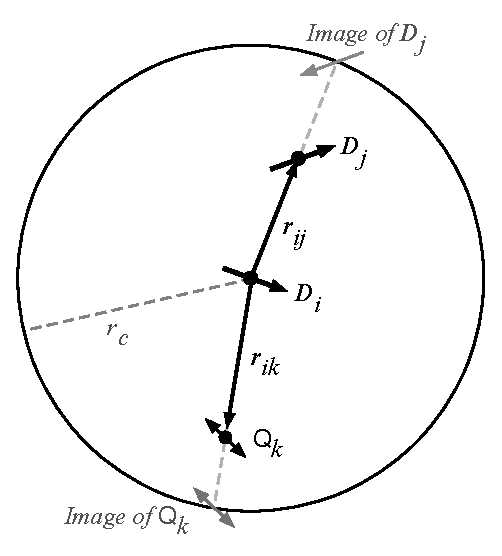
\includegraphics[scale=0.8]{SM.eps}}
    \caption{Reversed multipoles are projected onto the surface of the
  cutoff sphere. The forces, torques, and potential are then smoothly
  shifted to zero as the sites leave the cutoff region.}
    \label{fig:shiftedMultipoles}
  \end{center}
\end{figure}

As in the point-charge approach, there is an additional contribution
from self-neutralization of site $i$.  The self term for multipoles is
described in section \ref{sec:selfTerm}.

\subsection{The multipole expansion}

Consider two discrete rigid collections of point charges, denoted as objects
$a$ and $b$.  In the following, we assume that the two objects
interact via electrostatics only and describe those interactions in
terms of a standard multipole expansion.  Putting the origin of the
coordinate system at the center of mass of $a$, we use vectors
$\mathbf{r}_k$ to denote the positions of all charges $q_k$ in 
$a$.  Then the electrostatic potential of object $a$ at
$\mathbf{r}$ is given by
\begin{equation}
\phi_a(\mathbf r) = 
 \sum_{k \, \text{in } a} \frac{q_k}{\lvert \mathbf{r} - \mathbf{r}_k \rvert}.
\end{equation}
The Taylor expansion in $r$ can be written using an implied summation
notation.  Here Greek indices are used to indicate space coordinates
($x$, $y$, $z$) and the subscripts $k$ and $j$ are reserved for
labeling specific sites for charges in $a$ and $b$ respectively.  The
Taylor expansion,
\begin{equation}
 \frac{1}{\lvert \mathbf{r} - \mathbf{r}_k \rvert} = 
\left( 1
-  r_{k\alpha} \frac{\partial}{\partial r_{\alpha}} 
+ \frac{1}{2}  r_{k\alpha} r_{k\beta} \frac{\partial^2}{\partial r_{\alpha} \partial r_{\beta}} +\dots 
\right)
\frac{1}{r}  ,
\end{equation}
can then be used to express the electrostatic potential on $a$ in
terms of multipole operators,
\begin{equation}
\phi_a(\mathbf{r}) =M_a \frac{1}{r} 
\end{equation}
where
\begin{equation}
M_a = C_a - D_{a\alpha} \frac{\partial}{\partial r_{\alpha}} 
+  Q_{a\alpha\beta}
 \frac{\partial^2}{\partial r_{\alpha} \partial r_{\beta}} + \dots
\end{equation}
Here, the point charge, dipole, and quadrupole for object $a$ are
given by $C_a$, $\mathbf{D}_a$, and $\mathsf{Q}_a$, respectively.  These are the primitive multipoles
which can be expressed as a distribution of charges,
\begin{align}
C_a =&\sum_{k \, \text{in }a} q_k , \label{eq:charge} \\
D_{a\alpha} =&\sum_{k \, \text{in }a} q_k r_{k\alpha}, \label{eq:dipole}\\
Q_{a\alpha\beta} =& \frac{1}{2} \sum_{k \, \text{in }  a} q_k
r_{k\alpha}  r_{k\beta} . \label{eq:quadrupole}
\end{align}
Note that the definition of the primitive quadrupole here differs from
the standard traceless form, and contains an additional Taylor-series
based factor of $1/2$.  We are essentially treating the mass
distribution with higher priority; the moment of inertia tensor,
$\mathsf I$, is diagonalized to obtain body-fixed
axes, and the charge distribution may result in a quadrupole tensor
that is not necessarily diagonal in the body frame.  Additional
reasons for utilizing the primitive quadrupole are discussed in
section \ref{sec:damped}.

It is convenient to locate charges $q_j$ relative to the center of mass of  $b$.  Then with $\bf{r}$ pointing from
the center of mass of $a$ to the center of mass of $b$ ($\mathbf{r}=\mathbf{r}_b - \mathbf{r}_a $), the interaction energy is given by
\begin{equation}
U_{ab}(r)
= M_a \sum_{j \, \text{in } b} \frac {q_j}{\vert \mathbf{r}+\mathbf{r}_j \vert} .
\end{equation}
This can also be expanded as a Taylor series in $r$.  Using a notation
similar to before to define the multipoles in object  $b$,
\begin{equation}
M_b = C_b + D_{b\alpha} \frac{\partial}{\partial r_{\alpha}} 
+   Q_{b\alpha\beta}
 \frac{\partial^2}{\partial r_{\alpha} \partial r_{\beta}} + \dots
\end{equation}
we arrive at the multipole expression for the total interaction energy.
\begin{equation}
U_{ab}(r)=M_a M_b \frac{1}{r}  \label{kernel}.
\end{equation}
This form has the benefit of separating out the energies of
interaction into contributions from the charge, dipole, and quadrupole
of $a$ interacting with the same types of multipoles in $b$.

\subsection{Damped Coulomb interactions}
\label{sec:damped}
In the standard multipole expansion, one typically uses the bare
Coulomb potential, with radial dependence $1/r$, as shown in
Eq.~(\ref{kernel}).  It is also quite common to use a damped Coulomb
interaction, which results from replacing point charges with Gaussian
distributions of charge with width $\alpha$.  In damped multipole
electrostatics, the kernel ($1/r$) of the expansion is replaced with
the function:
\begin{equation}
B_0(r)=\frac{\text{erfc}(\alpha r)}{r} = \frac{2}{\sqrt{\pi}r}
\int_{\alpha r}^{\infty} \text{e}^{-s^2} ds .
\end{equation}
We develop equations below using the function $f(r)$ to represent
either $1/r$ or $B_0(r)$, and all of the techniques can be applied to
bare or damped Coulomb kernels (or any other function) as long as
derivatives of these functions are known.  Smith's convenient
functions $B_l(r)$, which are used for derivatives of the damped
kernel, are summarized in Appendix~\ref{SmithFunc} (N.B. there is one important
distinction between the two kernels, which is the behavior of
$\nabla^2 \frac{1}{r}$ compared with $\nabla^2 B_0(r)$.  The former is
zero everywhere except for a delta function evaluated at the origin.
The latter also has delta function behavior, but is non-zero for $r
\neq 0$.  Thus the standard justification for using a traceless
quadrupole tensor fails for the damped case.)

The main goal of this work is to smoothly cut off the interaction
energy as well as forces and torques as $r\rightarrow r_c$.  To
describe how this goal may be met, we use two examples, charge-charge
and charge-dipole, using the bare Coulomb kernel, $f(r)=1/r$, to
explain the idea.
\subsection{Shifted-force methods}
In the shifted-force approximation, the interaction energy for two
charges $C_a$ and $C_b$ separated by a distance $r$ is
written:
\begin{equation}
U_{C_aC_b}(r)= C_a C_b
\left({ \frac{1}{r} - \frac{1}{r_c} + (r - r_c) \frac{1}{r_c^2}  }
\right) .
\end{equation}
Two shifting terms appear in this equations, one from the
neutralization procedure ($-1/r_c$), and one that causes the first
derivative to vanish at the cutoff radius.

Since one derivative of the interaction energy is needed for the
force, the minimal perturbation is a term linear in $(r-r_c)$ in the
interaction energy, that is:
\begin{equation}
\frac{d\,}{dr} 
\left( {\frac{1}{r} - \frac{1}{r_c} + (r - r_c) \frac{1}{r_c^2}  }
\right) = \left(- \frac{1}{r^2} + \frac{1}{r_c^2} 
\right) .
\end{equation}
which clearly vanishes as the $r$ approaches the cutoff radius. There
are a number of ways to generalize this derivative shift for
higher-order multipoles.  Below, we present two methods, one based on
higher-order Taylor series for $r$ near $r_c$, and the other based on
linear shift of the kernel gradients at the cutoff itself.

\subsection{Taylor-shifted force (TSF) electrostatics}
In the Taylor-shifted force (TSF) method, the procedure that we follow
is based on a Taylor expansion containing the same number of
derivatives required for each force term to vanish at the cutoff.  For
example, the quadrupole-quadrupole interaction energy requires four
derivatives of the kernel, and the force requires one additional
derivative. For quadrupole-quadrupole interactions, we therefore
require shifted energy expressions that include up to $(r-r_c)^5$ so
that all energies, forces, and torques are zero as $r \rightarrow
r_c$. In each case, we subtract off a function $f_n^{\text{shift}}(r)$
from the kernel $f(r)=1/r$.  The subscript $n$ indicates the number of
derivatives to be taken when deriving a given multipole energy.  We
choose a function with guaranteed smooth derivatives -- a truncated
Taylor series of the function $f(r)$, e.g.,
%
\begin{equation}
f_n^{\text{shift}}(r)=\sum_{m=0}^{n+1} \frac {(r-r_c)^m}{m!} f^{(m)}(r_c)  .
\end{equation}
%
The combination of $f(r)$ with the shifted function is denoted $f_n(r)=f(r)-f_n^{\text{shift}}(r)$.
Thus, for $f(r)=1/r$, we find
%
\begin{equation}
f_1(r)=\frac{1}{r}- \frac{1}{r_c} + (r - r_c) \frac{1}{r_c^2} - \frac{(r-r_c)^2}{r_c^3} .
\end{equation}
%
Continuing with the example of a charge $a$ interacting with a
dipole $b$, we write
%
\begin{equation}
U_{C_a\mathbf{D}_b}(r)=
C_a D_{b\alpha}  \frac {\partial f_1(r) }{\partial r_\alpha} 
= C_a D_{b\alpha}
\frac {r_\alpha}{r} \frac {\partial f_1(r)}{\partial r} .
\end{equation}
%
The force that dipole  $ b$ exerts on charge $a$ is
%
\begin{equation}
F_{C_a \mathbf{D}_b \beta} = C_a D_{b \alpha}
\left[ \frac{\delta_{\alpha\beta}}{r} \frac {\partial}{\partial r} + 
\frac{r_\alpha r_\beta}{r^2}
\left( -\frac{1}{r} \frac {\partial} {\partial r} 
+ \frac {\partial ^2} {\partial r^2} \right) \right] f_1(r) .
\end{equation}
%
For undamped coulombic interactions, $f(r)=1/r$, we find
%
\begin{equation}
F_{C_a \mathbf{D}_b \beta} =
\frac{C_a D_{b\beta}}{r}
\left[  -\frac{1}{r^2}+\frac{1}{r_c^2}-\frac{2(r-r_c)}{r_c^3} \right] 
+C_a D_{b \alpha}r_\alpha r_\beta 
\left[ \frac{3}{r^5}-\frac{3}{r^3r_c^2} \right] .
\end{equation}
%
This expansion shows the expected $1/r^3$ dependence of the force.  

In general, we can write
%
\begin{equation}
U^{\text{TSF}}= (\text{prefactor}) (\text{derivatives}) f_n(r)
\label{generic}
\end{equation}
%
with $n=0$ for charge-charge, $n=1$ for charge-dipole, $n=2$ for
charge-quadrupole and dipole-dipole, $n=3$ for dipole-quadrupole, and
$n=4$ for quadrupole-quadrupole.  For example, in
quadrupole-quadrupole interactions for which the $\text{prefactor}$ is
$Q_{a \alpha\beta}Q_{b \gamma\delta}$, the derivatives are
$\partial^4/\partial r_\alpha \partial r_\beta \partial
r_\gamma \partial r_\delta$, with implied summation combining the
space indices.  Appendix \ref{radialTSF} contains details on the
radial functions.

In the formulas presented in the tables below, the placeholder
function $f(r)$ is used to represent the electrostatic kernel (either
damped or undamped).  The main functions that go into the force and
torque terms, $g_n(r), h_n(r), s_n(r), \mathrm{~and~} t_n(r)$ are
successive derivatives of the shifted electrostatic kernel, $f_n(r)$
of the same index $n$.  The algebra required to evaluate energies,
forces and torques is somewhat tedious, so only the final forms are
presented in Tables~\ref{tab:tableenergy} and \ref{tab:tableFORCE}.
One of the principal findings of our work is that the individual
orientational contributions to the various multipole-multipole
interactions must be treated with distinct radial functions, but each
of these contributions is independently force shifted at the cutoff
radius.  
\subsection{Gradient-shifted force (GSF) electrostatics}
The second, and conceptually simpler approach to force-shifting
maintains only the linear $(r-r_c)$ term in the truncated Taylor
expansion, and has a similar interaction energy for all multipole
orders:
\begin{equation}
U^{\text{GSF}} = \sum \left[ U(\mathbf{r}, \mathsf{A}, \mathsf{B}) -
U(r_c \hat{\mathbf{r}},\mathsf{A}, \mathsf{B}) - (r-r_c)
\hat{\mathbf{r}} \cdot \nabla U(r_c \hat{\mathbf{r}},\mathsf{A}, \mathsf{B}) \right]
\label{generic2}
\end{equation}
where $\hat{\mathbf{r}}$ is the unit vector pointing between the two
multipoles, and the sum describes a separate force-shifting that is
applied to each orientational contribution to the energy.  Both the
potential and the gradient for force shifting are evaluated for an
image multipole projected onto the surface of the cutoff sphere (see
fig \ref{fig:shiftedMultipoles}).  The image multipole retains the
orientation (rotation matrix $\mathsf{B}$) of the interacting multipole.  No
higher order terms $(r-r_c)^n$ appear.  The primary difference between
the TSF and GSF methods is the stage at which the Taylor Series is
applied; in the Taylor-shifted approach, it is applied to the kernel
itself.  In the Gradient-shifted approach, it is applied to individual
radial interaction terms in the multipole expansion.  Energies from
this method thus have the general form:
\begin{equation}
U= \sum  (\text{angular factor}) (\text{radial factor}).
\label{generic3}
\end{equation}

Functional forms for both methods (TSF and GSF) can both be summarized
using the form of Eq.~(\ref{generic3}).  The basic forms for the
energy, force, and torque expressions are tabulated for both shifting
approaches below -- for each separate orientational contribution, only
the radial factors differ between the two methods.

\subsection{Generalization of the Wolf shifted potential (SP)}
It is also possible to formulate an extension of the Wolf approach for
multipoles by simply projecting the image multipole onto the surface
of the cutoff sphere, and including the interactions with the central
multipole and the image.  This effectively shifts the pair potential
to zero at the cutoff radius,
\begin{equation}
U^{\text{SP}} = \sum \left[ U(\mathbf{r}, \mathsf{A}, \mathsf{B}) -
U(r_c \hat{\mathbf{r}},\mathsf{A}, \mathsf{B}) \right]
\label{eq:SP}
\end{equation}
independent of the orientations of the two multipoles.  The sum again
describes separate potential shifting that is applied to each
orientational contribution to the energy.
 
The shifted potential (SP) method is a simple truncation of the GSF
method for each orientational contribution, leaving out the $(r-r_c)$
terms that multiply the gradient. Functional forms for the
shifted-potential (SP) method can also be summarized using the form of
Eq.~\ref{generic3}.  The energy, force, and torque expressions are
tabulated below for all three methods. As in the GSF and TSF methods,
for each separate orientational contribution, only the radial factors
differ between the SP, GSF, and TSF methods.


\subsection{\label{sec:level2}Body and space axes}
Although objects $a$ and $b$ rotate during a molecular
dynamics (MD) simulation, their multipole tensors remain fixed in
body-frame coordinates. While deriving force and torque expressions,
it is therefore convenient to write the energies, forces, and torques
in intermediate forms involving the vectors of the rotation matrices.
We denote body axes for objects $a$ and $b$ using unit vectors
$\hat{\mathbf{A}}_m$ and $\hat{\mathbf{B}}_m$, respectively, with the index $m=(123)$.
In a typical simulation, the initial axes are obtained by
diagonalizing the moment of inertia tensors for the objects.  (N.B.,
the body axes are generally {\it not} the same as those for which the
quadrupole moment is diagonal.)  The rotation matrices are then
propagated during the simulation.

The rotation matrices $\mathsf {A}$ and $\mathsf {B}$ can be
expressed using these unit vectors:
\begin{eqnarray}
\mathsf {A} = 
\begin{pmatrix}
\hat{\mathbf{A}}_1 \\
\hat{\mathbf{A}}_2 \\
\hat{\mathbf{A}}_3
\end{pmatrix}, \qquad
\mathsf {B} = 
\begin{pmatrix}
\hat{\mathbf{B}}_1 \\
\hat{\mathbf{B}}_2 \\
\hat{\mathbf{B}}_3
\end{pmatrix}
\end{eqnarray}
%
These matrices convert from space-fixed $(xyz)$ to body-fixed $(123)$
coordinates.

Allen and Germano,\cite{Allen06} following earlier work by Price
{\em et al.},\cite{Price84} showed that if the interaction
energies are written explicitly in terms of $\hat{\mathbf{r}}$ and the body
axes ($\hat{\mathbf{A}}_m$, $\hat{\mathbf{B}}_n$) :
%
\begin{equation}
U(r, \{\hat{\mathbf{A}}_m \cdot \hat{\mathbf{r}} \}, 
\{\hat{\mathbf{B}}_n\cdot \hat{\mathbf{r}} \}, 
\{\hat{\mathbf{A}}_m \cdot \hat{\mathbf{B}}_n \}) .
\label{ugeneral}
\end{equation}
%
the forces come out relatively cleanly,
%
\begin{eqnarray}
\mathbf{F}_a &=&-\mathbf{F}_b =  \nabla U = \frac{\partial U}{\partial \mathbf{r}} \nonumber \\   
&=& \frac{\partial U}{\partial r} \hat{\mathbf{r}} 
 + \sum_m \left[ 
\frac{\partial U}{\partial (\hat{\mathbf{A}}_m \cdot \hat{\mathbf{r}})} 
\frac { \partial (\hat{\mathbf{A}}_m \cdot \hat{\mathbf{r}})}{\partial \mathbf{r}} 
+ \frac{\partial U}{\partial (\hat{\mathbf{B}}_m \cdot \hat{\mathbf{r}})} 
\frac { \partial (\hat{\mathbf{B}}_m \cdot \hat{\mathbf{r}})}{\partial \mathbf{r}} 
\right] \label{forceequation}.
\end{eqnarray}

The torques can also be found in a relatively similar
manner,
%
\begin{eqnarray}
\mathbf{\tau}_a =
 \sum_m 
\frac{\partial U}{\partial (\hat{\mathbf{A}}_m \cdot \hat{\mathbf{r}})} 
( \hat{\mathbf{r}} \times \hat{\mathbf{A}}_m )
-\sum_{mn}
\frac{\partial U}{\partial (\hat{\mathbf{A}}_m \cdot \hat{\mathbf{B}}_n)} 
(\hat{\mathbf{A}}_m \times \hat{\mathbf{B}}_n) \\
%
\mathbf{\tau}_b =
 \sum_m 
\frac{\partial U}{\partial (\hat{\mathbf{B}}_m \cdot \hat{\mathbf{r}})} 
( \hat{\mathbf{r}} \times \hat{\mathbf{B}}_m)
+\sum_{mn}
\frac{\partial U}{\partial (\hat{\mathbf{A}}_m \cdot \hat{\mathbf{B}}_n)} 
(\hat{\mathbf{A}}_m \times \hat{\mathbf{B}}_n) .
\end{eqnarray}

Note that our definition of $\mathbf{r}=\mathbf{r}_b - \mathbf{r}_a $
is opposite in sign to that of Allen and Germano.\cite{Allen06}
We also made use of the identities,
%
\begin{align}
\frac { \partial (\hat{\mathbf{A}}_m \cdot \hat{\mathbf{r}})}{\partial \mathbf{r}} 
=& \frac{1}{r} \left(  \hat{\mathbf{A}}_m - (\hat{\mathbf{A}}_m \cdot \hat{\mathbf{r}})\hat{\mathbf{r}}
\right) \\
\frac { \partial (\hat{\mathbf{B}}_m \cdot \hat{\mathbf{r}})}{\partial \mathbf{r}} 
=& \frac{1}{r} \left(  \hat{\mathbf{B}}_m - (\hat{\mathbf{B}}_m \cdot \hat{\mathbf{r}})\hat{\mathbf{r}} 
\right).
\end{align}

Many of the multipole contractions required can be written in one of
three equivalent forms using the unit vectors $\hat{\mathbf{r}}$, $\hat{\mathbf{A}}_m$,
and $\hat{\mathbf{B}}_n$. In the torque expressions, it is useful to have the
angular-dependent terms available in all three fashions, e.g. for the
dipole-dipole contraction:
%
\begin{equation}
 \mathbf{D}_a \cdot \mathbf{D}_b
= D_{a \alpha} D_{b \alpha} =
\sum_{mn} D_{am} \hat{\mathbf{A}}_m \cdot \hat{\mathbf{B}}_n D_{bn}.
\end{equation}
%
The first two forms are written using space coordinates.  The first
form is standard in the chemistry literature, while the second is
expressed using implied summation notation.  The third form shows
explicit sums over body indices and the dot products now indicate
contractions using space indices. 

In computing our force and torque expressions, we carried out most of
the work in body coordinates, and have transformed the expressions
back to space-frame coordinates, which are reported below.  Interested
readers may consult supplemental information of the Ref. \cite{PaperI} for the intermediate body-frame expressions.

\subsection{The Self-Interaction \label{sec:selfTerm}}

In addition to cutoff-sphere neutralization, the Wolf
summation~\cite{Wolf99} and the damped shifted force (DSF)
extension~\cite{Gezelter06} also include self-interactions that
are handled separately from the pairwise interactions between
sites. The self-term is normally calculated via a single loop over all
sites in the system, and is relatively cheap to evaluate. The
self-interaction has contributions from two sources.

First, the neutralization procedure within the cutoff radius requires
a contribution from a charge opposite in sign, but equal in magnitude,
to the central charge, which has been spread out over the surface of
the cutoff sphere.  For a system of undamped charges, the total
self-term is
\begin{equation}
U_\textrm{self} = - \frac{1}{r_c} \sum_{a=1}^N C_a^{2}.
\label{eq:selfTerm}
\end{equation}
The extension of DSF electrostatics to point multipoles requires
treatment of the self-neutralization \textit{and} reciprocal
contributions to the self-interaction for higher order multipoles.  In
this section we give formulae for these interactions up to quadrupolar
order.

The self-neutralization term is computed by taking the {\it
  non-shifted} kernel for each interaction, placing a multipole of
equal magnitude (but opposite in polarization) on the surface of the
cutoff sphere, and averaging over the surface of the cutoff sphere.
Because the self term is carried out as a single sum over sites, the
reciprocal-space portion is identical to half of the self-term
obtained by Smith, and also by Aguado and Madden for the application
of the Ewald sum to multipoles.\cite{Smith82,Smith98,Aguado03} For a
given site which possesses a charge, dipole, and quadrupole, both types
of contribution are given in Table~\ref{tab:tableSelf}.

\begin{table*}
\begin{center}
  \caption{\label{tab:tableSelf} Self-interaction contributions for 
    site ($a$) that has a charge $(C_a)$, dipole
    $(\mathbf{D}_a)$, and quadrupole $(\mathsf{Q}_a)$}.
\begin{ruledtabular}
\begin{tabular}{|l|c|c|c|} \hline
Multipole order & Summed Quantity & Self-neutralization  & Reciprocal \\ \hline
Charge & $C_a^2$ & $-f(r_c)$ & $-\frac{\alpha}{\sqrt{\pi}}$ \\
Dipole & $|\mathbf{D}_a|^2$ & $\frac{1}{3} \left( h(r_c) +
  \frac{2 g(r_c)}{r_c} \right)$ & $-\frac{2 \alpha^3}{3 \sqrt{\pi}}$\\
Quadrupole & $2 \mathsf{Q}_a:\mathsf{Q}_a + \text{Tr}(\mathsf{Q}_a)^2$ &
$- \frac{1}{15} \left( t(r_c)+ \frac{4 s(r_c)}{r_c} \right)$ &
$-\frac{4 \alpha^5}{5 \sqrt{\pi}}$ \\
Charge-Quadrupole & $-2 C_a \text{Tr}(\mathsf{Q}_a)$ & $\frac{1}{3} \left(
  h(r_c) + \frac{2 g(r_c)}{r_c} \right)$& $-\frac{2 \alpha^3}{3 \sqrt{\pi}}$ \\ \hline
\end{tabular}
\end{ruledtabular}
\end{center}
\end{table*}

For sites which simultaneously contain charges and quadrupoles, the
self-interaction includes a cross-interaction between these two
multipole orders.  Symmetry prevents the charge-dipole and
dipole-quadrupole interactions from contributing to the
self-interaction.  The functions that go into the self-neutralization
terms, $g(r), h(r), s(r), \mathrm{~and~} t(r)$ are successive
derivatives of the electrostatic kernel, $f(r)$ (either the undamped
$1/r$ or the damped $B_0(r)=\mathrm{erfc}(\alpha r)/r$ function) that
have been evaluated at the cutoff distance.  For undamped
interactions, $f(r_c) = 1/r_c$, $g(r_c) = -1/r_c^{2}$, and so on.  For
damped interactions, $f(r_c) = B_0(r_c)$, $g(r_c) = B_0'(r_c)$, and so
on.  Appendix \ref{SmithFunc} contains recursion relations that allow
rapid evaluation of these derivatives.

\section{Interaction energies, forces, and torques}
The main result of this chapter is a set of expressions for the
energies, forces and torques (up to quadrupole-quadrupole order) that
work for the Taylor-shifted, gradient-shifted, and shifted potential
approximations.  These expressions were derived using a set of generic
radial functions.  Without using the shifting approximations mentioned
above, some of these radial functions would be identical, and the
expressions coalesce into the familiar forms for unmodified
multipole-multipole interactions.  Table~\ref{tab:tableenergy} maps
between the generic functions and the radial functions derived for the
three methods.  The energy equations are written in terms of lab-frame
representations of the dipoles, quadrupoles, and the unit vector
connecting the two objects,

% Energy in space coordinate form ----------------------------------------------------------------------------------------------
%
%
% u ca cb
%
\begin{align}
U_{C_a C_b}(r)=&
C_a C_b  v_{01}(r)  \label{uchch}
\\
%
% u ca db
%
U_{C_a \mathbf{D}_b}(r)=&
C_a \left( \mathbf{D}_b \cdot \hat{\mathbf{r}} \right)  v_{11}(r)  
 \label{uchdip}
\\
%
% u ca qb
%
U_{C_a \mathsf{Q}_b}(r)=& C_a \Bigl[ \text{Tr}\mathsf{Q}_b
v_{21}(r) + \left( \hat{\mathbf{r}} \cdot \mathsf{Q}_b \cdot
  \hat{\mathbf{r}} \right) v_{22}(r) \Bigr]
\label{uchquad}
\\
%
% u da cb
%
%U_{D_{\bf a}C_{\bf b}}(r)=&
%-\frac{C_{\bf b}}{4\pi \epsilon_0}  
%\left( \mathbf{D}_{\mathbf{a}} \cdot \hat{r} \right)   v_{11}(r) \label{udipch}
%\\
%
% u da db
%
U_{\mathbf{D}_a \mathbf{D}_b}(r)=&
-\Bigr[ \left( \mathbf{D}_a \cdot
\mathbf{D}_b \right)  v_{21}(r)
+\left( \mathbf{D}_a \cdot \hat{\mathbf{r}} \right)
\left( \mathbf{D}_b \cdot \hat{\mathbf{r}} \right)  
v_{22}(r) \Bigr]
\label{udipdip}
\\
%
% u da qb
%
\begin{split}
% 1
U_{\mathbf{D}_a \mathsf{Q}_b}(r) =&
-\Bigl[
\text{Tr}\mathsf{Q}_b
\left( \mathbf{D}_a \cdot \hat{\mathbf{r}} \right)
+2 ( \mathbf{D}_a \cdot
\mathsf{Q}_b \cdot \hat{\mathbf{r}} ) \Bigr] v_{31}(r) \\
% 2
&- \left( \mathbf{D}_a \cdot \hat{\mathbf{r}} \right)
 \left( \hat{\mathbf{r}} \cdot \mathsf{Q}_b \cdot \hat{\mathbf{r}} \right) v_{32}(r)
\label{udipquad}
\end{split}
\\
%
% u qa cb
%
%U_{Q_{\bf a}C_{\bf b}}(r)=&
%\frac{C_{\bf b }}{4\pi \epsilon_0} \Bigl[ \text{Tr}\mathbf{Q}_{\bf a}  v_{21}(r)
%\left( \hat{r} \cdot \mathbf{Q}_{{\mathbf a}} \cdot \hat{r} \right)  v_{22}(r)  \Bigr]
%\label{uquadch}
%\\
%
% u qa db
%
%\begin{split}
%1
%U_{Q_{\bf a}D_{\bf b}}(r)=&
%\frac{1}{4\pi \epsilon_0} \Bigl[
%\text{Tr}\mathbf{Q}_{\mathbf{a}}
%\left(  \mathbf{D}_{\mathbf{b}} \cdot \hat{r} \right)
%+2 ( \mathbf{D}_{\mathbf{b}} \cdot 
%\mathbf{Q}_{\mathbf{a}}  \cdot \hat{r}) \Bigr] v_{31}(r)\\
% 2
%&+\frac{1}{4\pi \epsilon_0}
%\left(  \mathbf{D}_{\mathbf{b}} \cdot \hat{r} \right)
%\left( \hat{r} \cdot \mathbf{Q}_{{\mathbf a}} \cdot \hat{r} \right) v_{32}(r)
%\label{uquaddip}
%\end{split}
%\\
%
% u qa qb
%
\begin{split}
%1
U_{\mathsf{Q}_a \mathsf{Q}_b}(r)=&
\Bigl[
\text{Tr} \mathsf{Q}_a \text{Tr} \mathsf{Q}_b
+2
\mathsf{Q}_a : \mathsf{Q}_b \Bigr] v_{41}(r)
\\
% 2
&+\Bigl[ \text{Tr}\mathsf{Q}_a
 \left( \hat{\mathbf{r}} \cdot 
\mathsf{Q}_b \cdot \hat{\mathbf{r}} \right)
+\text{Tr}\mathsf{Q}_b
\left( \hat{\mathbf{r}} \cdot \mathsf{Q}_a
 \cdot \hat{\mathbf{r}} \right)  +4 (\hat{\mathbf{r}}  \cdot
\mathsf{Q}_a \cdot \mathsf{Q}_b \cdot \hat{\mathbf{r}})
\Bigr] v_{42}(r)
 \\
% 4
&+ 
\left( \hat{\mathbf{r}} \cdot  \mathsf{Q}_a \cdot \hat{\mathbf{r}} \right)
\left( \hat{\mathbf{r}} \cdot \mathsf{Q}_b  \cdot \hat{\mathbf{r}} \right) v_{43}(r).
\label{uquadquad}
\end{split}
\end{align}
%
Note that the energies of multipoles on site $b$ interacting
with those on site $a$ can be obtained by swapping indices
along with the sign of the intersite vector, $\hat{\mathbf{r}}$.

%
%
% TABLE of radial functions  ----------------------------------------------------------------------------------------------------------------
%

\begin{sidewaystable}
  \caption{\label{tab:tableenergy}Radial functions used in the energy
    and torque equations.  The $f, g, h, s, t, \mathrm{and~} u$
    functions used in this table are defined in Appendices
    \ref{radialTSF} and \ref{radialGSF}.  The gradient shifted (GSF)
    functions include the shifted potential (SP)
    contributions (\textit{cf.} Eqs.~\ref{generic2} and
    \ref{eq:SP}).}
\centering
\resizebox{\textwidth}{!}{\begin{tabular}{|c|c|l|l|l|} \hline
Generic&Bare Coulomb&Taylor-Shifted (TSF)&Shifted Potential (SP)&Gradient-Shifted (GSF)
\\ \hline
%
%
%
%Ch-Ch&
$v_{01}(r)$ &
$\frac{1}{r}$ &
$f_0(r)$ &
$f(r)-f(r_c)$ &
SP $-(r-r_c)g(r_c)$
\\
%
%
%
%Ch-Di&
$v_{11}(r)$ &
$-\frac{1}{r^2}$ &
$g_1(r)$ &
$g(r)-g(r_c)$ &
SP $-(r-r_c)h(r_c)$ \\
%
%
%
%Ch-Qu/Di-Di&
$v_{21}(r)$ &
$-\frac{1}{r^3}  $ & 
$\frac{g_2(r)}{r} $ &
$\frac{g(r)}{r}-\frac{g(r_c)}{r_c}$ &
SP $-(r-r_c) \left( -\frac{g(r_c)}{r_c^2} + \frac{h(r_c)}{r_c} \right)$ \\
%
%
%
$v_{22}(r)$ &
$\frac{3}{r^3}  $ &
$\left(-\frac{g_2(r)}{r} + h_2(r) \right)$ &
$\left(-\frac{g(r)}{r}+h(r) \right) -\left(-\frac{g(r_c)}{r_c}+h(r_c) \right)$ 
& SP $-(r-r_c) \left( \frac{g(r_c)}{r_c^2}-\frac{h(r_c)}{r_c}+s(r_c) \right)$\\
%
%
%
%Di-Qu &
$v_{31}(r)$ &
$\frac{3}{r^4}  $ &
$\left(-\frac{g_3(r)}{r^2} + \frac{h_3(r)}{r} \right)$ &
$\left( -\frac{g(r)}{r^2}+\frac{h(r)}{r}\right)-\left(-\frac{g(r_c)}{r_c^2}+\frac{h(r_c)}{r_c} \right)$ 
& SP $-(r-r_c) \left(\frac{2g(r_c)}{r_c^3}-\frac{2h(r_c)}{r_c^2}+\frac{s(r_c)}{r_c} \right)$  \\
% 
%
%
$v_{32}(r)$ &
$-\frac{15}{r^4}  $ &
$\left( \frac{3g_3(r)}{r^2} - \frac{3h_3(r)}{r} + s_3(r) \right)$ &
$\left( \frac{3g(r)}{r^2} - \frac{3h(r)}{r} + s(r) \right)$&
SP $-(r-r_c) \left( \frac{-6g(r_c)}{r_c^3}+\frac{6h(r_c)}{r_c^2}\right.$ \\
&&& $~~~-\left(\frac{3g(r_c)}{r_c^2} - \frac{3h(r_c)}{r_c} + s(r_c)\right)$ & 
$\phantom{SP-(r-r_c)}\left.-\frac{3s(r_c)}{r_c}+t(r_c) \right)$\\
%
%
%
%Qu-Qu&
$v_{41}(r)$ &
$\frac{3}{r^5} $ &
$\left(-\frac{g_4(r)}{r^3} +\frac{h_4(r)}{r^2} \right) $  &
$\left( -\frac{g(r)}{r^3} + \frac{h(r)}{r^2} \right)- \left(-\frac{g(r_c)}{r_c^3} + \frac{h(r_c)}{r_c^2} \right)$ & 
SP $-(r-r_c) \left( \frac{3g(r_c)}{r_c^4}-\frac{3h(r_c)}{r_c^3}+\frac{s(r_c)}{r_c^2} \right)$ 
\\
% 2
$v_{42}(r)$ &
$- \frac{15}{r^5}   $ &
$\left( \frac{3g_4(r)}{r^3} - \frac{3h_4(r)}{r^2}+\frac{s_4(r)}{r} \right)$ &
$\left( \frac{3g(r)}{r^3} - \frac{3h(r)}{r^2}+\frac{s(r)}{r} \right)$ & 
SP$-(r-r_c) \left(- \frac{9g(r_c)}{r_c^4}+\frac{9h(r_c)}{r_c^3}\right.$  \\
&&& $~~~-\left( \frac{3g(r_c)}{r_c^3} -  \frac{3h(r_c)}{r_c^2}+\frac{s(r_c)}{r_c} \right)$ & 
$\phantom{SP-(r-r_c)}\left. -\frac{4s(r_c)}{r_c^2} + \frac{t(r_c)}{r_c}\right)$\\
% 3
%
%
$v_{43}(r)$ &
$ \frac{105}{r^5}  $ &
$\left(-\frac{15g_4(r)}{r^3}+\frac{15h_4(r)}{r^2}-\frac{6s_4(r)}{r} + t_4(r)\right) $ &
$ \left(-\frac{15g(r)}{r^3} +\frac{15h(r)}{r^2}-\frac{6s(r)}{r}+t(r)\right) $ &
SP $-(r-r_c)\left(\frac{45g(r_c)}{r_c^4}-\frac{45h(r_c)}{r_c^3}\right.$\\
&&& $~~~-\left(-\frac{15g(r_c)}{r_c^3}+\frac{15h(r_c)}{r_c^2}-\frac{6s(r_c)}{r_c}+ t(r_c)\right)$ & 
$\phantom{SP-(r-r_c)}\left.+\frac{21s(r_c)}{r_c^2}-\frac{6t(r_c)}{r_c}+u(r_c) \right)$\\
\hline
\end{tabular}}
\end{sidewaystable}
%
%
% FORCE	 TABLE of radial functions  ----------------------------------------------------------------------------------------------------------------
%

\begin{sidewaystable}
\caption{\label{tab:tableFORCE}Radial functions used in the force
  equations. Gradient shifted (GSF) functions are constructed using the shifted
    potential (SP) functions.  Some of these functions are simple
    modifications of the functions found in Table~\ref{tab:tableenergy}}
\centering
\resizebox{\textwidth}{!}{\begin{tabular}{|c|c|l|l|l|} \hline
Function&Definition&Taylor-Shifted (TSF)& Shifted Potential (SP)
&Gradient-Shifted (GSF)
\\ \hline
%
%
%
$w_a(r)$&
$\frac{d v_{01}}{dr}$&
$g_0(r)$&
$g(r)$&
SP $-g(r_c)$ \\
%
%
$w_b(r)$ &
$\frac{d v_{11}}{dr} - \frac{v_{11}(r)}{r} $&
$\left( -\frac{g_1(r)}{r}+h_1(r) \right)$ &
$h(r) - \frac{v_{11}(r)}{r} $ &
SP $- h(r_c)$ \\
%
$w_c(r)$ &
$\frac{v_{11}(r)}{r}$ &
$\frac{g_1(r)}{r} $ &
$\frac{v_{11}(r)}{r}$&
$\frac{v_{11}(r)}{r}$\\
%
%
$w_d(r)$&
$\frac{d v_{21}}{dr}$&
$\left( -\frac{g_2(r)}{r^2} + \frac{h_2(r)}{r} \right) $ &
$\left( -\frac{g(r)}{r^2} + \frac{h(r)}{r} \right)$ &
SP $-\left( -\frac{g(r_c)}{r_c^2} + \frac{h(r_c)}{r_c} \right) $ \\
%
$w_e(r)$ &
$\frac{v_{22}(r)}{r}$&
$\left(-\frac{g_2(r)}{r^2} + \frac{h_2(r)}{r} \right)$ &
$\frac{v_{22}(r)}{r}$ &
$\frac{v_{22}(r)}{r}$ \\
% 
%
$w_f(r)$&
$\frac{d v_{22}}{dr} - \frac{2v_{22}(r)}{r}$&
$\left( \frac{3g_2(r)}{r^2}-\frac{3h_2(r)}{r}+s_2(r) \right)$ &
  $ \left( \frac{g(r)}{r^2}-\frac{h(r)}{r}+s(r) \right) -\frac{2v_{22}(r)}{r}$&
SP $- \left( \frac{g(r_c)}{r_c^2}-\frac{h(r_c)}{r_c}+s(r_c) \right)$\\
%
$w_g(r)$& 
$\frac{v_{31}(r)}{r}$& 
$ \left( -\frac{g_3(r)}{r^3}+\frac{h_3(r)}{r^2} \right)$& 
$\frac{v_{31}(r)}{r}$&
$\frac{v_{31}(r)}{r}$\\
%
$w_h(r)$ &
$\frac{d v_{31}}{dr} -\frac{v_{31}(r)}{r}$&
$\left(\frac{3g_3(r)}{r^3} -\frac{3h_3(r)}{r^2} +\frac{s_3(r)}{r} \right) $  &
$ \left(\frac{2g(r)}{r^3} -\frac{2h(r)}{r^2} +\frac{s(r)}{r} \right) -\frac{v_{31}(r)}{r}$ &
SP $ - \left(\frac{2g(r_c)}{r_c^3} -\frac{2h(r_c)}{r_c^2} +\frac{s(r_c)}{r_c} \right) $ \\
% 2
$w_i(r)$ &
$\frac{v_{32}(r)}{r}$ &
$\left(\frac{3g_3(r)}{r^3} -\frac{3h_3(r)}{r^2} +\frac{s_3(r)}{r} \right) $  &
$\frac{v_{32}(r)}{r}$&
$\frac{v_{32}(r)}{r}$\\
% 
$w_j(r)$ &
$\frac{d v_{32}}{dr}  - \frac{3v_{32}}{r}$&
$\left(\frac{-15g_3(r)}{r^3} + \frac{15h_3(r)}{r^2} - \frac{6s_3(r)}{r} + t_3(r) \right)  $ &
$\left(\frac{-6g(r)}{r^3} +\frac{6h(r)}{r^2} -\frac{3s(r)}{r} +t(r) \right) -\frac{3v_{32}}{r}$ &
SP $-\left(\frac{-6g(_cr)}{r_c^3} +\frac{6h(r_c)}{r_c^2}
  -\frac{3s(r_c)}{r_c} +t(r_c) \right)$ \\
%
$w_k(r)$ &
$\frac{d v_{41}}{dr} $ &
$\left(\frac{3g_4(r)}{r^4} -\frac{3h_4(r)}{r^3} +\frac{s_4(r)}{r^2}  \right)$ &
$\left(\frac{3g(r)}{r^4} -\frac{3h(r)}{r^3} +\frac{s(r)}{r^2}
\right)$ &
SP $-\left(\frac{3g(r_c)}{r_c^4} -\frac{3h(r_c)}{r_c^3} +\frac{s(r_c)}{r_c^2}  \right)$ \\
%
$w_l(r)$ &
$\frac{d v_{42}}{dr} -\frac{2v_{42}(r)}{r}$ &
$\left(-\frac{15g_4(r)}{r^4} +\frac{15h_4(r)}{r^3} -\frac{6s_4(r)}{r^2} +\frac{t_4(r)}{r} \right)$ &
$\left(-\frac{9g(r)}{r^4} +\frac{9h(r)}{r^3} -\frac{4s(r)}{r^2}
  +\frac{t(r)}{r} \right) -\frac{2v_{42}(r)}{r}$&
SP$-\left(-\frac{9g(r_c)}{r_c^4} +\frac{9h(r_c)}{r_c^3} -\frac{4s(r_c)}{r_c^2} +\frac{t(r_c)}{r_c} \right)$\\
%
$w_m(r)$ &
$\frac{d v_{43}}{dr} -\frac{4v_{43}(r)}{r}$&
$\left(\frac{105g_4(r)}{r^4} - \frac{105h_4(r)}{r^3} \right.$ &
$\left(\frac{45g(r)}{r^4} -\frac{45h(r)}{r^3} +\frac{21s(r)}{r^2}\right.$ &
SP $- \left(\frac{45g(r_c)}{r_c^4} -\frac{45h(r_c)}{r_c^3}\right.$ \\
&& $~~~\left.+ \frac{45s_4(r)}{r^2} - \frac{10t_4(r)}{r} +u_4(r) \right)$
& $~~~\left. -\frac{6t(r)}{r} +u(r) \right) -\frac{4v_{43}(r)}{r}$ &
$\phantom{SP-} \left.+\frac{21s(r_c)}{r_c^2} -\frac{6t(r_c)}{r_c} +u(r_c) \right) $\\ 
%
$w_n(r)$ &
$\frac{v_{42}(r)}{r}$ &
$\left(\frac{3g_4(r)}{r^4} -\frac{3h_4(r)}{r^3} +\frac{s_4(r)}{r^2}  \right)$ &
$\frac{v_{42}(r)}{r}$&
$\frac{v_{42}(r)}{r}$\\
%
$w_o(r)$ &
$\frac{v_{43}(r)}{r}$&
$\left(-\frac{15g_4(r)}{r^4} +\frac{15h_4(r)}{r^3} -\frac{6s_4(r)}{r^2} +\frac{t_4(r)}{r} \right)$ &
$\frac{v_{43}(r)}{r}$&
$\frac{v_{43}(r)}{r}$  \\ \hline
%

\end{tabular}}
\end{sidewaystable}


\subsection{Forces}
The force on object $a$, $\mathbf{F}_a$, due to object
$b$ is the negative of the force on $b$ due to $a$. For
a simple charge-charge interaction, these forces will point along the
$\pm \hat{\mathbf{r}}$ directions, where $\mathbf{r}=\mathbf{r}_b -
\mathbf{r}_a $.  Thus
%
\begin{equation}
F_{a \alpha} = \hat{r}_\alpha \frac{\partial U_{C_a C_b}}{\partial r} 
\quad \text{and} \quad  F_{b \alpha} 
= - \hat{r}_\alpha \frac{\partial U_{C_a C_b}} {\partial r}  .
\end{equation}
%
We list below the force equations written in terms of lab-frame
coordinates.  The radial functions used in the three methods are listed
in Table~\ref{tab:tableFORCE}
%
%SPACE COORDINATES FORCE EQUATIONS
%
% **************************************************************************
% f ca cb
%
\begin{align}
\mathbf{F}_{a {C_a} {C_b}} =&
C_a C_b  w_a(r) \hat{\mathbf{r}} \\
%
%
%
\mathbf{F}_{a {C_a} {\mathbf{D}_b} } =&
C_a \Bigl[
 \left( \hat{\mathbf{r}} \cdot \mathbf{D}_b  \right) 
w_b(r) \hat{\mathbf{r}}  
+ \mathbf{D}_b w_c(r) \Bigr] \\
%
%
%
\mathbf{F}_{a {C_a} {\mathsf{Q}_b}} =&
C_a \Bigr[
\text{Tr}\mathsf{Q}_b w_d(r) \hat{\mathbf{r}}
+ 2  \mathsf{Q}_b \cdot \hat{\mathbf{r}} w_e(r)
 + \left( \hat{\mathbf{r}} \cdot  \mathsf{Q}_b \cdot \hat{\mathbf{r}}
 \right) w_f(r) \hat{\mathbf{r}} \Bigr] \\
%
%
%
% \begin{equation}
% \mathbf{F}_{{\bf a}D_{\bf a}C_{\bf b}} = 
% -C_{\bf{b}} \Bigl[
% \left( \hat{r} \cdot  \mathbf{D}_{\mathbf{a}} \right) w_b(r) \hat{r}
% + \mathbf{D}_{\mathbf{a}} w_c(r) \Bigr]
% \end{equation}
%
%
%
\begin{split}
\mathbf{F}_{a \mathbf{D}_a \mathbf{D}_b} =&
- \mathbf{D}_a \cdot  \mathbf{D}_b w_d(r) \hat{\mathbf{r}}
+ \left( \mathbf{D}_a 
\left( \mathbf{D}_b \cdot \hat{\mathbf{r}} \right)
+ \mathbf{D}_b \left( \mathbf{D}_a  \cdot \hat{\mathbf{r}} \right) \right) w_e(r)\\
% 2
& - \left( \hat{\mathbf{r}} \cdot \mathbf{D}_a \right) 
\left( \hat{\mathbf{r}} \cdot \mathbf{D}_b \right) w_f(r) \hat{\mathbf{r}}
\end{split}\\
%
%
%
\begin{split}
\mathbf{F}_{a \mathbf{D}_a \mathsf{Q}_b} =& - \Bigl[
\text{Tr}\mathsf{Q}_b \mathbf{ D}_a
+2 \mathbf{D}_a \cdot 
\mathsf{Q}_b \Bigr] w_g(r)
 - \Bigl[
\text{Tr}\mathsf{Q}_b
\left( \hat{\mathbf{r}} \cdot  \mathbf{D}_a \right) 
+2 ( \mathbf{D}_a \cdot 
\mathsf{Q}_b \cdot \hat{\mathbf{r}}) \Bigr] w_h(r) \hat{\mathbf{r}}  \\
% 3
& - \Bigl[\mathbf{ D}_a  (\hat{\mathbf{r}} \cdot \mathsf{Q}_b \cdot \hat{\mathbf{r}}) 
+2  (\hat{\mathbf{r}} \cdot \mathbf{D}_a ) (\hat{\mathbf{r}} \cdot \mathsf{Q}_b )  \Bigr]
w_i(r)
% 4
 -
(\hat{\mathbf{r}} \cdot \mathbf{D}_a )
(\hat{\mathbf{r}} \cdot \mathsf{Q}_b \cdot \hat{\mathbf{r}}) w_j(r) \hat{\mathbf{r}} \end{split} \\
%
%
% \begin{equation}
% \mathbf{F}_{{\bf a}Q_{\bf a}C_{\bf b}} = 
% \frac{C_{\bf b }}{4\pi \epsilon_0} \Bigr[
% \text{Tr}\mathbf{Q}_{\bf a} w_d(r) \hat{r}
% + 2  \mathbf{Q}_{{\mathbf a}} \cdot \hat{r} w_e(r)
%  + \left( \hat{r} \cdot  \mathbf{Q}_{{\mathbf a}} \cdot \hat{r} \right) w_f(r) \hat{r} \Bigr]
% \end{equation}
% %
% \begin{equation}
% \begin{split}
% \mathbf{F}_{{\bf a}Q_{\bf a}D_{\bf b}} = 
% &\frac{1}{4\pi \epsilon_0} \Bigl[
% \text{Tr}\mathbf{Q}_{\mathbf{a}} \mathbf{D}_{\mathbf{b}} 
% +2 \mathbf{D}_{\mathbf{b}} \cdot \mathbf{Q}_{\mathbf{a}}  \Bigr] w_g(r)
% % 2
% + \frac{1}{4\pi \epsilon_0} \Bigl[ \text{Tr}\mathbf{Q}_{\mathbf{a}}
% (\hat{r} \cdot  \mathbf{D}_{\mathbf{b}})
% +2 (\mathbf{D}_{\mathbf{b}} \cdot 
% \mathbf{Q}_{\mathbf{a}} \cdot \hat{r}) \Bigr] w_h(r) \hat{r}  \\
% % 3
% &+ \frac{1}{4\pi \epsilon_0} \Bigl[ \mathbf{D}_{\mathbf{b}} 
% (\hat{r} \cdot \mathbf{Q}_{{\mathbf a}} \cdot \hat{r}) 
% +2  (\hat{r} \cdot \mathbf{D}_{\mathbf{b}})
% (\hat{r} \cdot  \mathbf{Q}_{{\mathbf a}} ) \Bigr]   w_i(r)
% % 4
% +\frac{1}{4\pi \epsilon_0} 
% (\hat{r} \cdot \mathbf{D}_{\mathbf{b}}) 
% (\hat{r} \cdot \mathbf{Q}_{{\mathbf a}}  \cdot \hat{r}) w_j(r) \hat{r} 
% \end{split}
% \end{equation}
%
%
%
\begin{split}
\mathbf{F}_{a \mathsf{Q}_a \mathsf{Q}_b} =& 
 \Bigl[
\text{Tr}\mathsf{Q}_a \text{Tr}\mathsf{Q}_b 
+ 2  \mathsf{Q}_a :  \mathsf{Q}_b \Bigr] w_k(r) \hat{\mathbf{r}} \\
% 2
&+ \Bigl[
2\text{Tr}\mathsf{Q}_b  (\hat{\mathbf{r}} \cdot \mathsf{Q}_a )  
+ 2\text{Tr}\mathsf{Q}_a  (\hat{\mathbf{r}} \cdot \mathsf{Q}_b ) 
% 3
+4 (\mathsf{Q}_a  \cdot  \mathsf{Q}_b \cdot \hat{\mathbf{r}})  
+  4(\hat{\mathbf{r}} \cdot \mathsf{Q}_a \cdot \mathsf{Q}_b) \Bigr] w_n(r) \\
% 4
&+  \Bigl[
\text{Tr}\mathsf{Q}_a (\hat{\mathbf{r}} \cdot \mathsf{Q}_b \cdot \hat{\mathbf{r}}) 
+ \text{Tr}\mathsf{Q}_b
(\hat{\mathbf{r}} \cdot \mathsf{Q}_a  \cdot \hat{\mathbf{r}})  
% 5
+4 (\hat{\mathbf{r}} \cdot \mathsf{Q}_a \cdot  
\mathsf{Q}_b   \cdot \hat{\mathbf{r}}) \Bigr] w_l(r) \hat{\mathbf{r}} \\
%
&+ \Bigl[
+ 2 (\hat{\mathbf{r}} \cdot \mathsf{Q}_a )
(\hat{\mathbf{r}} \cdot \mathsf{Q}_b \cdot \hat{\mathbf{r}})
%6
+2 (\hat{\mathbf{r}} \cdot \mathsf{Q}_a \cdot \hat{\mathbf{r}})
(\hat{\mathbf{r}} \cdot \mathsf{Q}_b ) \Bigr] w_o(r) \\
%  7
&+ 
(\hat{\mathbf{r}} \cdot \mathsf{Q}_a  \cdot \hat{\mathbf{r}}) 
(\hat{\mathbf{r}} \cdot \mathsf{Q}_b \cdot \hat{\mathbf{r}}) w_m(r) \hat{\mathbf{r}} \end{split}
\end{align}
Note that the forces for higher multipoles on site $a$
interacting with those of lower order on site $b$ can be
obtained by swapping indices in the expressions above.

%
% Torques SECTION -----------------------------------------------------------------------------------------
\subsection{Torques}

%
The torques for the three methods are given in space-frame
coordinates:
%
%
\begin{align}
\mathbf{\tau}_{b C_a \mathbf{D}_b} =& 
C_a  (\hat{\mathbf{r}} \times  \mathbf{D}_b) v_{11}(r) \\
%
%
%
\mathbf{\tau}_{b C_a \mathsf{Q}_b} =&
2C_a
\hat{\mathbf{r}} \times ( \mathsf{Q}_b \cdot \hat{\mathbf{r}}) v_{22}(r) \\
%
%
%
% \begin{equation}
% \mathbf{\tau}_{{\bf a}D_{\bf a}C_{\bf b}} =  
% -\frac{C_{\bf b}}{4\pi \epsilon_0}  
% (\hat{r} \times \mathbf{D}_{\mathbf{a}})  v_{11}(r) 
% \end{equation}
%
%
%
\mathbf{\tau}_{a \mathbf{D}_a \mathbf{D}_b} =&
 \mathbf{D}_a  \times \mathbf{D}_b v_{21}(r)
% 2
-
(\hat{\mathbf{r}} \times \mathbf{D}_a )
(\hat{\mathbf{r}} \cdot \mathbf{D}_b )  v_{22}(r)\\
%
%
%
% \begin{equation}
% \mathbf{\tau}_{{\bf b}D_{\bf a}D_{\bf b}} = 
% -\frac{1}{4\pi \epsilon_0} \mathbf{D}_{\mathbf {a}} \times \mathbf{D}_{\mathbf{b}} v_{21}(r)
% % 2
% +\frac{1}{4\pi \epsilon_0} 
% (\hat{r} \cdot \mathbf{D}_{\mathbf {a}} )
% (\hat{r} \times \mathbf{D}_{\mathbf {b}} ) v_{22}(r)
% \end{equation}
%
%
%
\mathbf{\tau}_{a \mathbf{D}_a \mathsf{Q}_b} =& 
 \Bigl[
-\text{Tr}\mathsf{Q}_b
(\hat{\mathbf{r}} \times \mathbf{D}_a )
+2 \mathbf{D}_a  \times 
(\mathsf{Q}_b \cdot \hat{\mathbf{r}})
\Bigr] v_{31}(r)
% 3
- (\hat{\mathbf{r}} \times \mathbf{D}_a )
(\hat{\mathbf{r}} \cdot \mathsf{Q}_b \cdot \hat{\mathbf{r}}) v_{32}(r)\\
%
%
%
\mathbf{\tau}_{b \mathbf{D}_a \mathsf{Q}_b} =&
 \Bigl[
+2 ( \mathbf{D}_a \cdot \mathsf{Q}_b ) \times
\hat{\mathbf{r}} 
-2 \mathbf{D}_a  \times 
(\mathsf{Q}_b \cdot \hat{\mathbf{r}})
\Bigr] v_{31}(r)
% 2
+
(\hat{\mathbf{r}} \cdot \mathbf{D}_a)
(\hat{\mathbf{r}} \cdot \mathsf{Q}_b) \times \hat{\mathbf{r}} v_{32}(r)\\
%
%
%
% \begin{equation}
% \mathbf{\tau}_{{\bf a}Q_{\bf a}D_{\bf b}} =
% \frac{1}{4\pi \epsilon_0} \Bigl[
% -2 (\mathbf{D}_{\mathbf{b}}  \cdot \mathbf{Q}_{\mathbf{a}} ) \times \hat{r} 
% +2 \mathbf{D}_{\mathbf{b}}  \times 
% (\mathbf{Q}_{\mathbf{a}}  \cdot \hat{r})
% \Bigr] v_{31}(r)
% % 3
% - \frac{2}{4\pi \epsilon_0}
% (\hat{r} \cdot \mathbf{D}_{\mathbf{b}} )
% (\hat{r} \cdot  \mathbf
% {Q}_{{\mathbf a}}) \times \hat{r} v_{32}(r)
% \end{equation}
%
%
%
% \begin{equation}
% \mathbf{\tau}_{{\bf b}Q_{\bf a}D_{\bf b}} = 
% \frac{1}{4\pi \epsilon_0} \Bigl[
% \text{Tr}\mathbf{Q}_{\mathbf{a}}
% (\hat{r} \times \mathbf{D}_{\mathbf{b}} )
% +2 \mathbf{D}_{\mathbf{b}}  \times
% ( \mathbf{Q}_{\mathbf{a}} \cdot \hat{r}) \Bigr] v_{31}(r)
% % 2
% +\frac{1}{4\pi \epsilon_0}
% (\hat{r} \times \mathbf{D}_{\mathbf{b}} )
% (\hat{r} \cdot \mathbf{Q}_{{\mathbf a}} \cdot \hat{r}) v_{32}(r)
% \end{equation}
%
%
%
\begin{split}
\mathbf{\tau}_{a \mathsf{Q}_a \mathsf{Q}_b} =&
-4 
\mathsf{Q}_a \times \mathsf{Q}_b
v_{41}(r) \\
% 2
&+ 
\Bigl[-2\text{Tr}\mathsf{Q}_b
(\hat{\mathbf{r}} \cdot \mathsf{Q}_a ) \times \hat{\mathbf{r}}
+4 \hat{\mathbf{r}} \times 
( \mathsf{Q}_a \cdot \mathsf{Q}_b \cdot \hat{\mathbf{r}}) 
% 3
-4 (\hat{\mathbf{r}} \cdot \mathsf{Q}_a )\times 
( \mathsf{Q}_b \cdot \hat{\mathbf{r}} ) \Bigr] v_{42}(r) \\
% 4
&+ 2
\hat{\mathbf{r}} \times ( \mathsf{Q}_a \cdot \hat{\mathbf{r}})
(\hat{\mathbf{r}} \cdot \mathsf{Q}_b \cdot \hat{\mathbf{r}}) v_{43}(r) \end{split}\\
%
%
%
\begin{split}
\mathbf{\tau}_{b \mathsf{Q}_a \mathsf{Q}_b} =  
&4
\mathsf{Q}_a \times \mathsf{Q}_b v_{41}(r) \\
% 2
&+  \Bigl[- 2\text{Tr}\mathsf{Q}_a
(\hat{\mathbf{r}} \cdot \mathsf{Q}_b ) \times \hat{\mathbf{r}}
-4  (\hat{\mathbf{r}} \cdot \mathsf{Q}_a \cdot 
\mathsf{Q}_b ) \times
\hat{\mathbf{r}} 
+4 ( \hat{\mathbf{r}} \cdot \mathsf{Q}_a ) \times 
( \mathsf{Q}_b \cdot \hat{\mathbf{r}})
\Bigr] v_{42}(r) \\
% 4
&+2
(\hat{\mathbf{r}} \cdot \mathsf{Q}_a \cdot \hat{\mathbf{r}})
\hat{\mathbf{r}} \times ( \mathsf{Q}_b \cdot \hat{\mathbf{r}}) v_{43}(r)\end{split}
\end{align}
%
Here, we have defined the matrix cross product in an identical form
as in Ref. \cite{Smith98}:
\begin{equation}
\left[\mathsf{A} \times \mathsf{B}\right]_\alpha = \sum_\beta
\left[\mathsf{A}_{\alpha+1,\beta} \mathsf{B}_{\alpha+2,\beta}
  -\mathsf{A}_{\alpha+2,\beta} \mathsf{B}_{\alpha+1,\beta} 
\right]
\label{eq:matrixCross}
\end{equation}
where $\alpha+1$ and $\alpha+2$ are regarded as cyclic
permuations of the matrix indices.

All of the radial functions required for torques are identical with
the radial functions previously computed for the interaction energies.
These are tabulated for all three methods in Table~\ref{tab:tableenergy}.  The torques for higher multipoles on site
$a$ interacting with those of lower order on site
$b$ can be obtained by swapping indices in the expressions
above.
\section{Comparison to known multipolar energies}

To understand how these new real-space multipole methods behave in
computer simulations, it is vital to test against established methods
for computing electrostatic interactions in periodic systems, and to
evaluate the size and sources of any errors that arise from the
real-space cutoffs. In this chapter we test SP, TSF, and GSF
electrostatics against analytical methods for computing the energies
of ordered multipolar arrays.  In the following chapter, we test the new
methods against the multipolar Ewald sum for computing the energies,
forces and torques for a wide range of typical condensed-phase
(disordered) systems.

Because long-range electrostatic effects can be significant in
crystalline materials, ordered multipolar arrays present one of the
biggest challenges for real-space cutoff methods.  The dipolar
analogues to the Madelung constants were first worked out by Sauer,
who computed the energies of ordered dipole arrays of zero
magnetization and obtained a number of these constants.\cite{Sauer}
This theory was developed more completely by Luttinger and
Tisza\cite{LT,LT2} who tabulated energy constants for the Sauer arrays
and other periodic structures.  

To test the new electrostatic methods, we have constructed very large,
$N=$ 16,000~(bcc) arrays of dipoles in the orientations described in
Ref. \cite{LT}.  These structures include ``A'' lattices with
nearest neighbor chains of antiparallel dipoles, as well as ``B''
lattices with nearest neighbor strings of antiparallel dipoles if the
dipoles are contained in a plane perpendicular to the dipole direction
that passes through the dipole.  We have also studied the minimum
energy structure for the BCC lattice that was found by Luttinger \&
Tisza.  The total electrostatic energy density for any of the arrays
is given by:
\begin{equation}
  E = C N^2 \mu^2
\end{equation}
where $C$ is the energy constant (equivalent to the Madelung
constant), $N$ is the number of dipoles per unit volume, and $\mu$ is
the strength of the dipole. Energy constants (converged to 1 part in
$10^9$) are given in the supplemental information Ref. \cite{PaperI}.
\begin{figure}[tpb]
  \begin{center}
    \centerline{\includegraphics[width = \linewidth]{Dipoles_rcut_threeAlpha.pdf}}
    \caption{Convergence of the lattice energy constants as a function of
  cutoff radius (normalized by the lattice constant, $a$) for the new
  real-space methods.  Three dipolar crystal structures were sampled,
  and the analytic energy constants for the three lattices are
  indicated with grey dashed lines.  The left panel shows results for
  the undamped kernel ($1/r$), while the damped kernel, $B_0(r)$ was
  used in the center and right panels.}
\label{fig:Dipoles_rCut}
  \end{center}
\end{figure}

For the purposes of testing the energy expressions and the
self-neutralization schemes, the primary quantity of interest is the
analytic energy constant for the perfect arrays.  Convergence to these
constants are shown as a function of the cutoff radius, $r_c$, for
three different values of the damping coefficient, $\alpha$ in
Fig.\ref{fig:Dipoles_rCut}.  We have simultaneously tested a hard
cutoff (where the kernel is simply truncated at the cutoff radius) in
addition to the three new methods.

The hard cutoff exhibits oscillations around the analytic energy
constants, and converges to incorrect energies when the complementary
error function damping kernel is used.  The shifted potential (SP)
converges to the correct energy smoothly by $r_c = 4.5 a$ even for the
undamped case. This indicates that the shifting and the correction
provided by the self term are required for obtaining accurate
energies. The Taylor-shifted force (TSF) approximation appears to
perturb the potential too much inside the cutoff region to provide
accurate measures of the energy constants.  GSF is a compromise,
converging to the correct energies within $r_c = 6 a$.

{\it Quadrupolar} analogues to the Madelung constants were first
worked out by Nagai and Nakamura who computed the energies of selected
quadrupole arrays based on extensions to the Luttinger and Tisza
approach.\cite{Nagai60,Nagai63} 

In analogy to the dipolar arrays, the total electrostatic energy for
the quadrupolar arrays is:
\begin{equation}
 E = C N \frac{3\bar{Q}^2}{4a^5} 
\end{equation} 
where $a$ is the lattice parameter, and $\bar{Q}$ is the effective
quadrupole moment,
\begin{equation}
\bar{Q}^2 = 2 \left(3 \mathsf{Q} : \mathsf{Q} - (\text{Tr} \mathsf{Q})^2 \right)
\end{equation}
for the primitive quadrupole as defined in Eq. \ref{eq:quadrupole}.
(For the traceless quadrupole tensor, $\mathsf{\Theta} = 3 \mathsf{Q} - \text{Tr} \mathsf{Q}$,
the effective moment, $\bar{Q}^2 = \frac{2}{3} \mathsf{\Theta} : \mathsf{\Theta}$.)

To test the new electrostatic methods for quadrupoles, we have
constructed very large, $N=$ 8,000~(sc), 16,000~(bcc), and
32,000~(fcc) arrays of linear quadrupoles in the orientations
described in Ref. \cite{Nagai60}.  We have compared the
energy constants for these low-energy configurations for linear
quadrupoles. Convergence to these constants are shown as a function of
the cutoff radius, $r_c$, for three different values of the damping
parameter, $\alpha$ in Fig.~\ref{fig:Quadrupoles_rCut}.

\begin{figure}
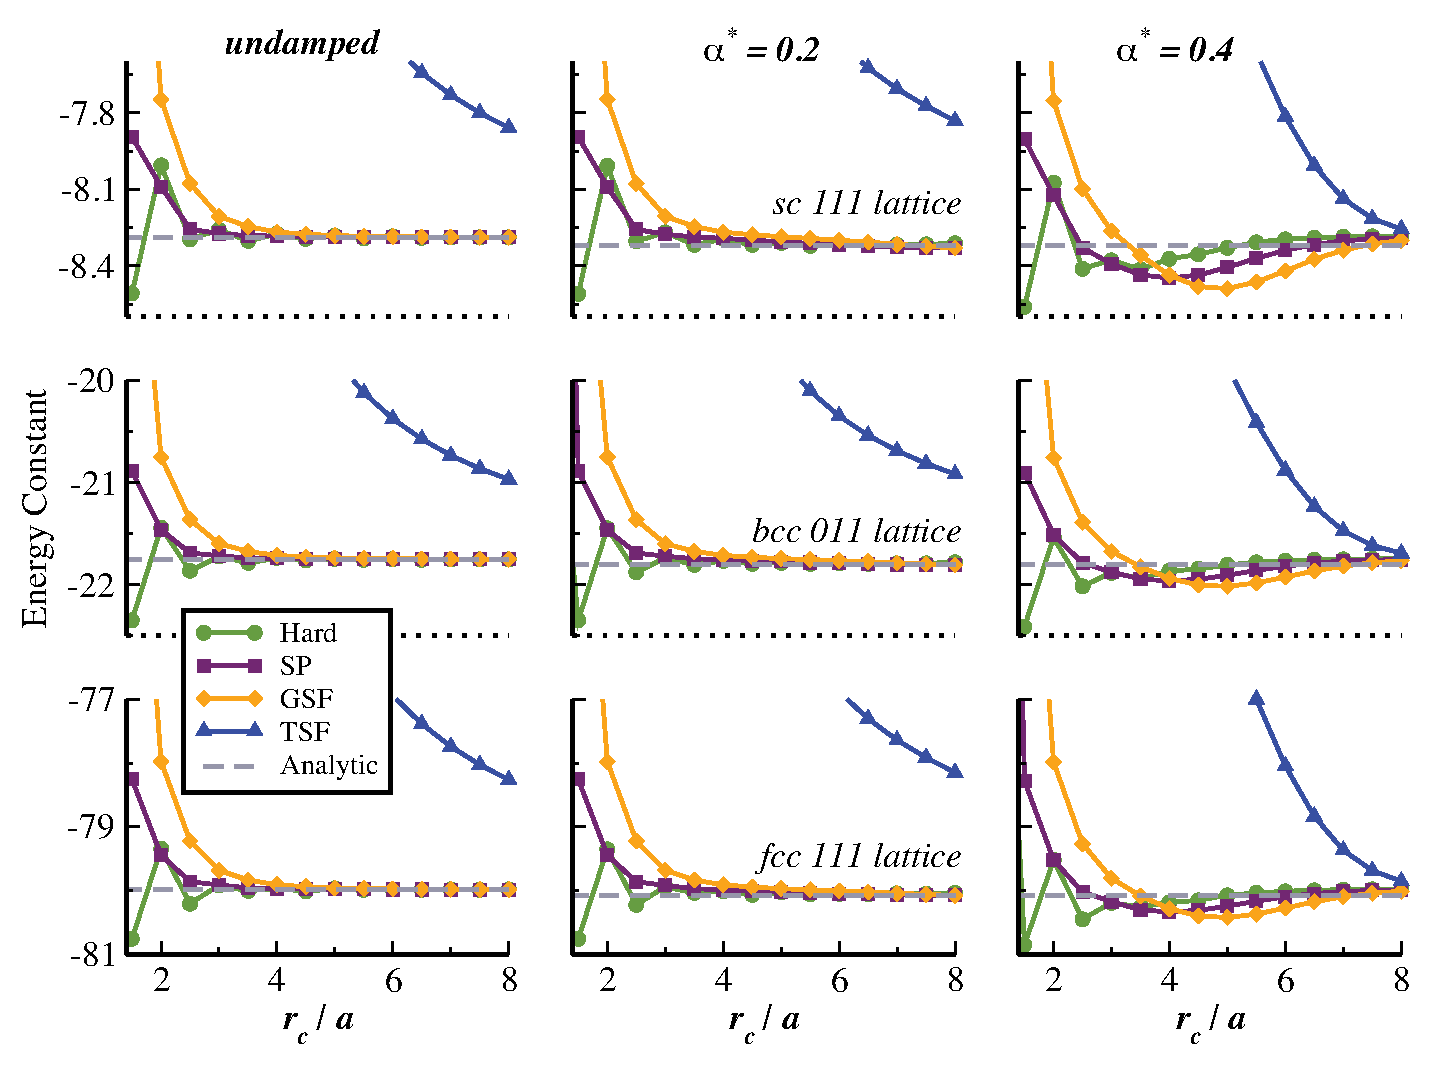
\includegraphics[width=\linewidth]{Quadrupoles_rcut_threeAlpha.eps}
\caption{Convergence of the lattice energy constants as a function of
  cutoff radius (normalized by the lattice constant, $a$) for the new
  real-space methods. Three quadrupolar crystal structures were
  sampled, and the analytic energy constants for the three lattices
  are indicated with grey dashed lines. The left panel shows results
  for the undamped kernel ($1/r$), while the damped kernel, $B_0(r)$
  was used in the center and right panels.  Note that for quadrupoles,
  $\alpha^* = 0.4$ overdamps contributions from repulsive orientations
  in the perfect crystal.}
\label{fig:Quadrupoles_rCut}
\end{figure}

Again, we find that the hard cutoff exhibits oscillations around the
analytic energy constants.  The shifted potential (SP) approximation
converges to the correct energy smoothly by $r_c = 3 a$ even for the
undamped case.  The Taylor-shifted force (TSF) approximation again
appears to perturb the potential too much inside the cutoff region to
provide accurate measures of the energy constants.  GSF again provides
a compromise between the two methods -- energies are converged by $r_c
= 4.5 a$, and the approximation is not as perturbative at short range
as TSF.

It is also useful to understand the behavior of the lattice energy
constants for different values of the reduced damping parameter
($\alpha^* = \alpha a$) for the real-space methods. All of the methods
(except for TSF) have excellent behavior for the undamped or
weakly-damped cases.  Overdamping can cause problems in perfect
crystals for the quadrupoles in particular ({\it cf.} the right panel
in Fig. \ref{fig:Quadrupoles_rCut}). In the perfect crystals, only a
few orientations are being sampled.  E.g. in the simple cubic (SC)
lattice of linear quadrupoles aligned in the 111 direction, the
nearest-neighbor quadrupoles only sample 3 distinct orientations
relative to the vector between the sites.  The damping alters the
radial function for the direct quadrupolar contraction, $v_{41}(r)$,
differently than the radial functions for the terms involving the
product of the separation vector with the quadrupoles, $v_{42}(r)$ and
$v_{43}(r)$.  Because these terms are altered by different amounts by
the complementary error function damping, the effect of damping is
non-spherical for multipoles, and the balance between attractive and
repulsive interactions in the crystal is therefore altered
significantly in overdamped situations.

In the chapter 3, we discuss how large values of
$\alpha$ can perturb the force and torque vectors, but weakly-damped
electrostatics appear to generate reasonable values for the total
electrostatic energies under both the SP and GSF approximations.  We
also discuss the effects that $\alpha$ can have on convergence to the
average electrostatic energies in liquids (which sample a much wider
range of local orientations).

\section{Summary}
We have presented three efficient real-space methods for computing the
interactions between point multipoles.  One of these (SP) is a
multipolar generalization of Wolf's method that smoothly shifts
electrostatic energies to zero at the cutoff radius. Two of these
methods (GSF and TSF) also smoothly truncate the forces and torques
(in addition to the energies) at the cutoff radius, making them
attractive for both molecular dynamics and Monte Carlo simulations. We
find that the Gradient-Shifted Force (GSF) and the Shifted-Potential
(SP) methods converge rapidly to the correct lattice energies for
ordered dipolar and quadrupolar arrays, while the Taylor-Shifted Force
(TSF) is too severe an approximation to provide convergence to lattice
energies within reasonable cutoff radii.

Although the TSF method appears to perform poorly for the analytical
energy constants, the structure of the radial functions used in the
force and torque expressions in the other two methods would not have
been revealed without first developing the TSF approach.  TSF also
generates a set of electrostatic kernels that have multiple
derivatives that vanish at the cutoff radius, a property that is
valuable in estimating dielectric constants using the conducting
boundary fluctuation formula.\cite{Izvekov08}

In most cases, GSF can obtain nearly quantitative agreement with the
lattice energy constants with reasonably small cutoff radii.  The only
exception we have observed is for crystals which exhibit a bulk
macroscopic dipole moment (e.g. Luttinger \& Tisza's $Z_1$ lattice).
In this particular case, the multipole neutralization scheme can
interfere with the correct computation of the energies.  We note that
the energies for these arrangements are typically much larger than for
crystals with net-zero moments, so this is not expected to be an issue
in most simulations.

Relatively weak damping is sufficient to converge to the analytical
energy constants within moderately short cutoff distances. Because
overdamping can present additional issues with higher order
multipoles, our results indicate that the damping coefficient should
be taken as small as possible, and that the {\it undamped} GSF and SP
methods may be the best choice in crystalline systems.

The techniques used here to derive the force, torque and energy
expressions can be extended to higher order multipoles, although some
of the objects (e.g. the matrix cross product in
Eq. \ref{eq:matrixCross}) will need to be generalized for higher-rank
tensors.  We also note that the definitions of the multipoles used
here are in a primitive form, and these need some care when comparing
with experiment or other computational techniques.

In large systems, these new methods can be made to scale approximately
linearly with system size, and detailed comparisons with the Ewald sum
for a wide range of chemical environments follows in the chapter 3.

%
%
%
%
% % uncomment the following lines,
% if using chapter-wise bibliography
%
% \bibliographystyle{ndnatbib}
% \bibliography{example}

%
% Chapter 3

%
% Modified by Megan Patnott
% Last Change: Jan 18, 2013
%
%%%%%%%%%%%%%%%%%%%%%%%%%%%%%%%%%%%%%%%%%%%%%%%%%%%%%%%%%%%%%%%%%%%%%%%%
%
% Modified by Sameer Vijay
% Last Change: Wed Jul 27 2005 13:00 CEST
%
%%%%%%%%%%%%%%%%%%%%%%%%%%%%%%%%%%%%%%%%%%%%%%%%%%%%%%%%%%%%%%%%%%%%%%%%
%
% Sample Notre Dame Thesis/Dissertation
% Using Donald Peterson's ndthesis classfile
%
% Written by Jeff Squyres and Don Peterson
%
% Provided by the Information Technology Committee of
%   the Graduate Student Union
%   http://www.gsu.nd.edu/
%
% Nothing in this document is serious except the format.  :-)
%
% If you have any suggestions, comments, questions, please send e-mail
% to: ndthesis@gsu.nd.edu
%
%%%%%%%%%%%%%%%%%%%%%%%%%%%%%%%%%%%%%%%%%%%%%%%%%%%%%%%%%%%%%%%%%%%%%%%%

%
% Chapter 3
%

\chapter{COMPARISONS WITH THE EWALD SUM}
\label{chap:compEwald}

In the previous chapter, I briefly discussed the short-ranged nature of the electrostatic interaction in the crystalline environment. This chapter discusses the property of the electrostatic interactions in more detail and extend the idea of the short-ranged nature of the interaction in the case of liquid simulation. I present the comparison of the energies, forces and torques calculated using real-space methods with the Ewald sum. Additionally I derive different static and dynamic properties using newly developed real-space methods and compare result with the Ewald. Finally I report on the conservation of total energy in the molecular dynamics simulation for the various real-space and Ewald methods.  

\section{Introduction}

As we mentioned earlier Wolf \textit{et al.}\cite{Wolf99} proposed a real space $O(N)$ method for calculating electrostatic interactions between point charges. They argued that the effective Coulomb interaction in most condensed phase systems is effectively short
ranged.\cite{Wolf92,Wolf95} For an ordered lattice (e.g., when
computing the Madelung constant of an ionic solid), the material can
be considered as a set of ions interacting with neutral dipolar or
quadrupolar ``molecules'' giving an effective distance dependence for
the electrostatic interactions of $r^{-5}$ (see Fig.~\ref{fig:schematic1}). If one views the \ce{NaCl} crystal as a simple
cubic (SC) structure with an octupolar \ce{$\mathrm{(NaCl)_4$}} basis, the
electrostatic energy per ion converges more rapidly to the Madelung
energy than the dipolar approximation.\cite{Wolf92} To find the
correct Madelung constant, Lacman suggested that the NaCl structure
could be constructed in a way that the finite crystal terminates with
complete \ce{$\mathrm{(NaCl)_4$}} molecules.\cite{Lacman65} The central ion sees
what is effectively a set of octupoles at large distances. These facts
suggest that the Madelung constants are relatively short ranged for
perfect ionic crystals.\cite{Wolf99} For this reason, careful
application of Wolf's method can provide accurate estimates of
Madelung constants using relatively short cutoff radii.

Direct truncation of interactions at a cutoff radius creates numerical
errors.  Wolf \textit{et al.} suggest that truncation errors are due
to net charge remaining inside the cutoff sphere.\cite{Wolf99} To
neutralize this charge they proposed placing an image charge on the
surface of the cutoff sphere for every real charge inside the cutoff sphere. These charges are present for the evaluation of both the pair
interaction energy and the force, although the force expression
maintains a discontinuity at the cutoff sphere.  In the original Wolf
formulation, the total energy for the charge and image were not equal
to the integral of the force expression, and as a result, the total
energy would not be conserved in molecular dynamics (MD)
simulations.\cite{Zahn02} Zahn \textit{et al.}, and Fennell and
Gezelter later proposed shifted force variants of the Wolf method with
commensurate force and energy expressions that do not exhibit this
problem.\cite{Zahn02,Gezelter06} Related real-space methods
were also proposed by Chen \textit{et al.} \cite{Chen04,Chen06,Denesyuk08,Rodgers06}
and by Wu and Brooks.\cite{Wu05} Recently, Fukuda has successfully
used additional neutralization of higher order moments for systems of
point charges.\cite{Fukuda13}

\begin{figure}
  \centering
  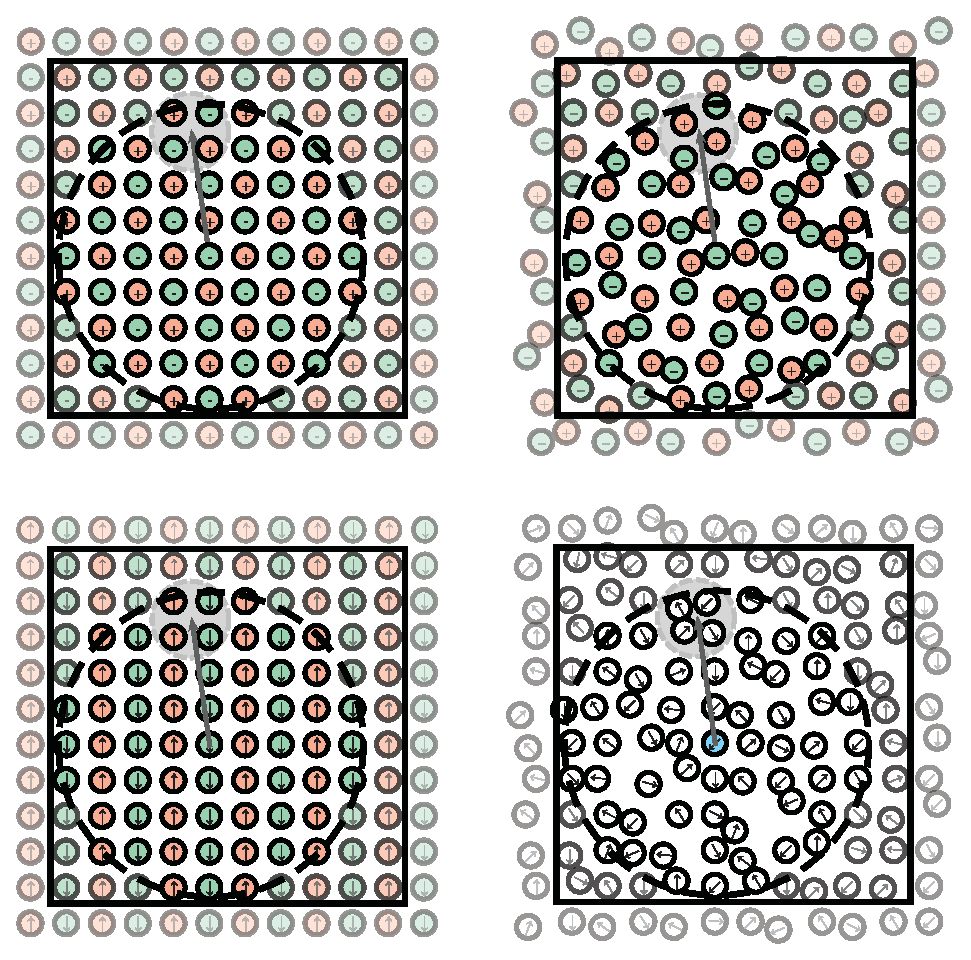
\includegraphics[width=\linewidth]{schematic.eps}
  \caption{Top: Ionic systems exhibit local clustering of dissimilar
    charges (in the smaller grey circle), so interactions are
    effectively charge-multipole at longer distances.  With hard
    cutoffs, motion of individual charges in and out of the cutoff
    sphere can break the effective multipolar ordering.  Bottom:
    dipolar crystals and fluids have a similar effective
    \textit{quadrupolar} ordering (in the smaller grey circles), and
    orientational averaging helps to reduce the effective range of the
    interactions in the fluid.  Placement of reversed image multipoles
    on the surface of the cutoff sphere recovers the effective
    higher-order multipole behavior. \label{fig:schematic1}}
\end{figure}

One can make a similar effective range argument for crystals of point
\textit{multipoles}. The Luttinger and Tisza treatment of energy
constants for dipolar lattices utilizes 24 basis vectors that contain
dipoles at the eight corners of a unit cube.\cite{LT} Only three of
these basis vectors, $X_1, Y_1, \mathrm{~and~} Z_1,$ retain net dipole
moments, while the rest have zero net dipole and retain contributions
only from higher order multipoles.  The lowest-energy crystalline
structures are built out of basis vectors that have only residual
quadrupolar moments (e.g. the $Z_5$ array). In these low energy
structures, the effective interaction between a dipole at the center
of a crystal and a group of eight dipoles farther away is
significantly shorter ranged than the $r^{-3}$ that one would expect
for raw dipole-dipole interactions.  Only in crystals which retain a
bulk dipole moment (e.g. ferroelectrics) does the analogy with the
ionic crystal break down -- ferroelectric dipolar crystals can exist,
while ionic crystals with net charge in each unit cell would be
unstable.

In ionic crystals, real-space truncation can break the effective
multipolar arrangements (see Fig. \ref{fig:schematic1}), causing
significant swings in the electrostatic energy as individual ions move
back and forth across the boundary.  This is why the image charges are
necessary for the Wolf sum to exhibit rapid convergence.  Similarly,
the real-space truncation of point multipole interactions breaks
higher order multipole arrangements, and image multipoles are required
for real-space treatments of electrostatic energies.

The shorter effective range of electrostatic interactions is not
limited to perfect crystals, but can also apply in disordered fluids.
Even at elevated temperatures, there is local charge balance in an
ionic liquid, where each positive ion has surroundings dominated by
negative ions and vice versa.  The reversed-charge images on the
cutoff sphere that are integral to the Wolf and damped shifted force
(DSF) approaches retain the effective multipolar interactions as the
charges traverse the cutoff boundary.

In multipolar fluids (see Fig. \ref{fig:schematic1}) there is
significant orientational averaging that additionally reduces the
effect of long-range multipolar interactions.  The image multipoles
that are introduced in the Taylor shifted force (TSF), gradient
shifted force (GSF), and shifted potential (SP) methods mimic this effect and reduce the effective range of the multipolar interactions as
interacting molecules traverse each other's cutoff boundaries.

Forces and torques acting on atomic sites are fundamental in driving
dynamics in molecular simulations, and the DSF energy kernel provides
consistent energies and forces on charged atoms within the cutoff
sphere. Both the energy and the force go smoothly to zero as an atom
approaches the cutoff radius. The comparisons of the accuracy these
quantities between the DSF kernel and SPME was surprisingly
good.\cite{Gezelter06} As a result, the DSF method has seen
increasing use in molecular systems with relatively uniform charge
densities. \cite{English08,Kannam13,Forrest12,Louden13,McCann13,Shi13,Tokumasu13}

\section{Methodology}
To understand how the real-space multipole methods behave in computer
simulations, it is vital to test against established methods for
computing electrostatic interactions in periodic systems, and to
evaluate the size and sources of any errors that arise from the
real-space cutoffs.  In the chapter 2 of this series, we compared
the dipolar and quadrupolar energy expressions against analytic
expressions for ordered dipolar and quadrupolar
arrays.\cite{Sauer,LT,Nagai60,Nagai63} In this work, we
used the multipolar Ewald sum as a reference method for comparing
energies, forces, and torques for molecular models that mimic
disordered and ordered condensed-phase systems.  The parameters used
in the test cases are given in Table~\ref{tab:pars}. 

\begin{sidewaystable}
  \caption{The parameters used in the systems used to evaluate the new
    real-space methods.  The most comprehensive test was a liquid
    composed of 2000 soft DQ liquid molecules with 48 dissolved ions (24 \ce{Na+} and 24 \ce{Cl-}
    ions).  This test exercises all orders of the multipolar
    interactions developed in the chapter 2.\label{tab:pars}}
\begin{tabularx}{\textwidth}{r|cc|YYccc|Yccc} \hline
             & \multicolumn{2}{c|}{LJ parameters} &
             \multicolumn{5}{c|}{Electrostatic moments} & & & & \\
 Test system & $\sigma$& $\epsilon$ & $C$ & $D$  &
 $Q_{xx}$ & $Q_{yy}$ & $Q_{zz}$ & mass  & $I_{xx}$ & $I_{yy}$ &
 $I_{zz}$ \\ \cline{6-8}\cline{10-12}
 & (\AA) & (kcal/mol) & (e) & (debye) & \multicolumn{3}{c|}{(debye \AA)} & (amu) & \multicolumn{3}{c}{(amu
 \AA\textsuperscript{2})} \\ \hline
    Soft Dipolar fluid & 3.051 & 0.152 &  & 2.35 & & & & 18.0153 & 1.77&0.6145& 1.155 \\
    Soft Dipolar solid & 2.837 & 1.0   &  & 2.35 & & & & $10^4$  & 17.6 &17.6 & 0 \\
Soft Quadrupolar fluid & 3.051 & 0.152 &  &  & -1&-1&-2.5 & 18.0153 & 1.77&0.6145&1.155  \\
Soft Quadrupolar solid & 2.837 & 1.0   &  &  & -1&-1&-2.5 & $10^4$  & 17.6&17.6&0 \\
      Soft DQ liquid  & 3.051 & 0.152 &  & 2.35 & -1.35&0&-0.68 & 18.0153 & 1.77&0.6145&1.155 \\
              \ce{Na+} & 2.579 & 0.118 & +1& & & & & 22.99 & & &\\
              \ce{Cl-} & 4.445 & 0.1   & -1& & & & & 35.4527& & & \\ \hline
\end{tabularx}
\end{sidewaystable}

The systems consist of pure multipolar solids (both dipole and
quadrupole), pure multipolar liquids (both dipole and quadrupole), a
fluid composed of sites containing both dipoles and quadrupoles
simultaneously, and a final test case that includes ions with point
charges in addition to the multipolar fluid.  The solid-phase
parameters were chosen so that the systems can explore some
orientational freedom for the multipolar sites, while maintaining
relatively strict translational order.  The soft DQ liquid model used
here based loosely on the SSDQO water
model,\cite{Chowdhuri06,Te10vn,Te10ys} but is not itself a
particularly accurate water model.  However, the soft DQ model does
test dipole-dipole, dipole-quadrupole, and quadrupole-quadrupole
interactions at roughly the same magnitudes. The last test case, a
soft DQ liquid with dissolved ions, exercises \textit{all} levels of
the multipole-multipole interactions we have derived so far and
represents the most complete test of the new methods.

In the following section, we present results for the total
electrostatic energy, as well as the electrostatic contributions to
the force and torque on each molecule.  These quantities have been
computed using the SP, TSF, and GSF methods, as well as a hard cutoff,
and have been compared with the values obtained from the multipolar
Ewald sum.  In Monte Carlo (MC) simulations, the energy differences
between two configurations is the primary quantity that governs how
the simulation proceeds. These differences are the most important
indicators of the reliability of a method even if the absolute
energies are not exact.  For each of the multipolar systems listed
above, we have compared the change in electrostatic potential energy
($\Delta E$) between 250 statistically-independent configurations.  In
molecular dynamics (MD) simulations, the forces and torques govern the
behavior of the simulation, so we also compute the electrostatic
contributions to the forces and torques.

\subsection{Implementation}
The real-space methods developed in the chapter 2 in this series
have been implemented in our group's open source molecular simulation
program, OpenMD,\cite{openmd} which was used for all calculations in
this work.  The complementary error function can be a relatively slow
function on some processors, so all of the radial functions are
precomputed on a fine grid and are spline-interpolated to provide
values when required.  

Using the same simulation code, we compare to a multipolar Ewald sum
with a reciprocal space cutoff, $k_\mathrm{max} = 7$.  Our version of
the Ewald sum is a re-implementation of the algorithm originally
proposed by Smith that does not use the particle mesh or smoothing
approximations.\cite{Smith82,Smith98} This implementation was tested
extensively against the analytic energy constants for the multipolar
lattices that are discussed in reference.\cite{PaperI} In all
cases discussed below, the quantities being compared are the
electrostatic contributions to energies, force, and torques.  All
other contributions to these quantities (i.e. from Lennard-Jones
interactions) are removed prior to the comparisons.

The convergence parameter ($\alpha$) also plays a role in the balance
of the real-space and reciprocal-space portions of the Ewald
calculation.  Typical molecular mechanics packages set this to a value
that depends on the cutoff radius and a tolerance (typically less than
$1 \times 10^{-4}$ kcal/mol).  Smaller tolerances are typically
associated with increasing accuracy at the expense of computational
time spent on the reciprocal-space portion of the
summation.\cite{Perram88,Essmann95} A default tolerance of $1 \times
10^{-8}$ kcal/mol was used in all Ewald calculations, resulting in
Ewald coefficient 0.3119 \AA$^{-1}$ for a cutoff radius of 12 \AA.

The real-space models have self-interactions that provide
contributions to the energies only.  Although the self interaction is
a rapid calculation, we note that in systems with fluctuating charges
or point polarizabilities, the self-term is not static and must be
recomputed at each time step.

\subsection{Model systems}
To sample independent configurations of the multipolar crystals, body
centered cubic (bcc) crystals, which exhibit the minimum energy
structures for point dipoles, were generated using 3,456 molecules.
The multipoles were translationally locked in their respective crystal
sites for equilibration at a relatively low temperature (50K) so that
dipoles or quadrupoles could freely explore all accessible
orientations.  The translational constraints were then removed, the
systems were re-equilibrated, and the crystals were simulated for an
additional 10 ps in the microcanonical (NVE) ensemble with an average
temperature of 50 K.  The balance between moments of inertia and
particle mass were chosen to allow orientational sampling without
significant translational motion.  Configurations were sampled at
equal time intervals in order to compare configurational energy
differences.  The crystals were simulated far from the melting point
in order to avoid translational deformation away of the ideal lattice
geometry.

For dipolar, quadrupolar, and mixed-multipole \textit{liquid}
simulations, each system was created with 2,048 randomly-oriented
molecules.  These were equilibrated at a temperature of 300K for 1 ns.
Each system was then simulated for 1 ns in the microcanonical (NVE)
ensemble with the Dullweber, Leimkuhler, and McLachlan (DLM)
symplectic splitting integrator using 1 fs
timesteps.\cite{Dullweber97} We collected 250 different
configurations at equal time intervals. For the liquid system that
included ionic species, we converted 48 randomly-distributed molecules
into 24 \ce{Na+} and 24 \ce{Cl-} ions and re-equilibrated. After
equilibration, the system was run under the same conditions for 1
ns. A total of 250 configurations were collected. In the following
comparisons of energies, forces, and torques, the Lennard-Jones
potentials were turned off and only the purely electrostatic
quantities were compared with the same values obtained via the Ewald
sum.

\subsection{Accuracy of Energy Differences, Forces and Torques}
The pairwise summation techniques (outlined above) were evaluated for
use in MC simulations by studying the energy differences between
different configurations.  We took the Ewald-computed energy
difference between two conformations to be the correct behavior. An
ideal performance by one of the new methods would reproduce these
energy differences exactly. The configurational energies being used
here contain only contributions from electrostatic interactions.
Lennard-Jones interactions were omitted from the comparison as they
should be identical for all methods.

Since none of the real-space methods provide exact energy differences,
we used least square regressions analysis for the six different
molecular systems to compare $\Delta E$ from Hard, SP, GSF, and TSF
with the multipolar Ewald reference method.  A result of unity for
both the correlation (slope) and coefficient of determination ($R^2$)
for these regressions would indicate perfect agreement between the
real-space method and the multipolar Ewald sum.

Molecular systems were run long enough to explore independent
configurations and 250 configurations were recorded for comparison.
Each system provided 31,125 energy differences for a total of 186,750
data points.  Similarly, the magnitudes of the forces and torques have
also been compared using least squares regression analysis. In the
forces and torques comparison, the magnitudes of the forces acting in
each molecule for each configuration were evaluated. For example, our
dipolar liquid simulation contains 2048 molecules and there are 250
different configurations for each system resulting in 3,072,000 data
points for comparison of forces and torques.

\subsection{Analysis of vector quantities}
Getting the magnitudes of the force and torque vectors correct is only
part of the issue for carrying out accurate molecular dynamics
simulations.  Because the real space methods reweight the different
orientational contributions to the energies, it is also important to
understand how the methods impact the \textit{directionality} of the
force and torque vectors. Fisher developed a probability density
function to analyse directional data sets,
\begin{equation}
p_f(\theta) = \frac{\kappa}{2 \sinh\kappa}\sin\theta e^{\kappa \cos\theta}
\label{eq:pdf}
\end{equation}
where $\kappa$ measures directional dispersion of the data around the
mean direction.\cite{Fisher53} This quantity $(\kappa)$ can be
estimated as a reciprocal of the circular variance.\cite{Allen91} To
quantify the directional error, forces obtained from the Ewald sum
were taken as the mean (or correct) direction and the angle between
the forces obtained via the Ewald sum and the real-space methods were
evaluated,
\begin{equation}
  \cos\theta_i =  \frac{\mathbf{f}_i^\mathrm{~Ewald} \cdot
    \mathbf{f}_i^\mathrm{~GSF}}{\left|\mathbf{f}_i^\mathrm{~Ewald}\right| \left|\mathbf{f}_i^\mathrm{~GSF}\right|}
\end{equation}
The total angular displacement of the vectors was calculated as,
\begin{equation}
R = \sqrt{\left(\sum\limits_{i=1}^N \cos\theta_i\right)^2 + \left(\sum\limits_{i=1}^N \sin\theta_i\right)^2}
\label{eq:displacement}
\end{equation} 
where $N$ is number of force vectors.  The circular variance is
defined as
\begin{equation}
\mathrm{Var}(\theta) \approx 1/\kappa = 1 - R/N
\end{equation}
The circular variance takes on values between from 0 to 1, with 0
indicating a perfect directional match between the Ewald force vectors
and the real-space forces. Lower values of $\mathrm{Var}(\theta)$
correspond to higher values of $\kappa$, which indicates tighter
clustering of the real-space force vectors around the Ewald forces.

A similar analysis was carried out for the electrostatic contribution
to the molecular torques as well as forces.  

\subsection{Energy conservation}
To test conservation the energy for the methods, the mixed molecular
system of 2000 soft DQ liquid molecules with 24 \ce{Na+} and 24
\ce{Cl-} ions was run for 1 ns in the microcanonical ensemble at an
average temperature of 300K.  Each of the different electrostatic
methods (Ewald, Hard, SP, GSF, and TSF) was tested for a range of
different damping values. The molecular system was started with same
initial positions and velocities for all cutoff methods. The energy
drift ($\delta E_1$) and standard deviation of the energy about the
slope ($\delta E_0$) were evaluated from the total energy of the
system as a function of time.  Although both measures are valuable at
investigating new methods for molecular dynamics, a useful interaction
model must allow for long simulation times with minimal energy drift.

\section{\label{sec:result}Results}
\subsection{Configurational energy differences}
 
\begin{figure}
  \centering
  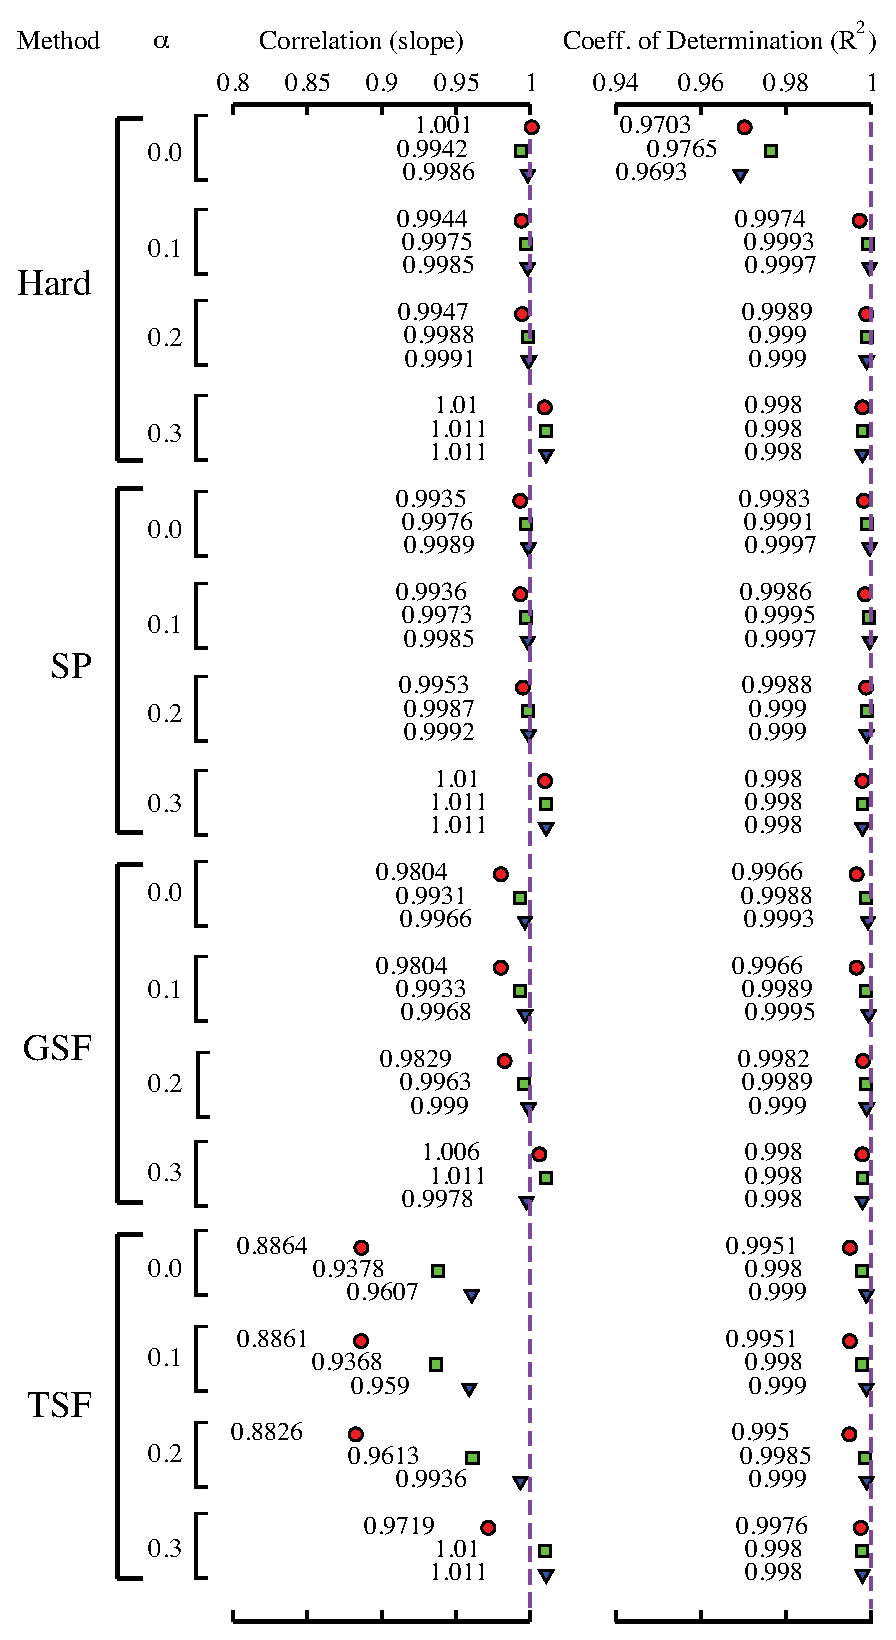
\includegraphics[width=0.6\linewidth]{energyPlot_slopeCorrelation_combined.eps}
  \caption{Statistical analysis of the quality of configurational
    energy differences for the real-space electrostatic methods
    compared with the reference Ewald sum.  Results with a value equal
    to 1 (dashed line) indicate $\Delta E$ values indistinguishable
    from those obtained using the multipolar Ewald sum.  Different
    values of the cutoff radius are indicated with different symbols
    (9~\AA\ = circles, 12~\AA\ = squares, and 15~\AA\ = inverted
    triangles).\label{fig:slopeCorr_energy}}
\end{figure} 

The combined coefficient of determination and slope for all six
systems is shown in Fig.~\ref{fig:slopeCorr_energy}.  Most of the
methods reproduce the Ewald configurational energy differences with
remarkable fidelity.  Undamped hard cutoffs introduce a significant
amount of random scatter in the energy differences which is apparent
in the reduced value of $R^2$ for this method.  This can be easily
understood as configurations which exhibit small traversals of a few
dipoles or quadrupoles out of the cutoff sphere will see large energy
jumps when hard cutoffs are used.  The orientations of the multipoles
(particularly in the ordered crystals) mean that these energy jumps
can go in either direction, producing a significant amount of random
scatter, but no systematic error.

The TSF method produces energy differences that are highly correlated
with the Ewald results, but it also introduces a significant
systematic bias in the values of the energies, particularly for
smaller cutoff values. The TSF method alters the distance dependence
of different orientational contributions to the energy in a
non-uniform way, so the size of the cutoff sphere can have a large
effect, particularly for the crystalline systems.

Both the SP and GSF methods appear to reproduce the Ewald results with
excellent fidelity, particularly for moderate damping ($\alpha \approx
0.2$~\AA$^{-1}$) and with a commonly-used cutoff value ($r_c =
12$~\AA).  With the exception of the undamped hard cutoff, and the TSF
method with short cutoffs, all of the methods would be appropriate for
use in Monte Carlo simulations.
\subsection{Magnitude of the force and torque vectors}

The comparisons of the magnitudes of the forces and torques for the
data accumulated from all six systems are shown in Fig.
~\ref{fig:slopeCorr_force} and \ref{fig:slopeCorr_torque}. The
correlation and slope for the forces agree well with the Ewald sum
even for the hard cutoffs.

For systems of molecules with only multipolar interactions, the pair
energy contributions are quite short ranged.  Moreover, the force
decays more rapidly than the electrostatic energy, hence the hard
cutoff method can also produce reasonable agreement for this quantity.
Although the pure cutoff gives reasonably good electrostatic forces
for pairs of molecules included within each other's cutoff spheres,
the discontinuity in the force at the cutoff radius can potentially
cause energy conservation problems as molecules enter and leave the
cutoff spheres.  This is discussed in detail in section
\ref{sec:conservation}.

The two shifted-force methods (GSF and TSF) exhibit a small amount of
systematic variation and scatter compared with the Ewald forces.  The
shifted-force models intentionally perturb the forces between pairs of
molecules inside each other's cutoff spheres in order to correct the
energy conservation issues, and this perturbation is evident in the
statistics accumulated for the molecular forces.  The GSF
perturbations are minimal, particularly for moderate damping and
commonly-used cutoff values ($r_c = 12$~\AA).  The TSF method shows
reasonable agreement in $R^2$, but again the systematic error in the
forces is concerning if replication of Ewald forces is desired.

It is important to note that the forces and torques from the SP and
the Hard cutoffs are not identical. The SP method shifts each
orientational contribution separately (e.g. the dipole-dipole dot
product is shifted by a different function than the dipole-distance
products), while the hard cutoff contains no orientation-dependent
shifting.  The forces and torques for these methods therefore diverge
for multipoles even though the forces for point charges are identical.

\begin{figure}
  \centering
  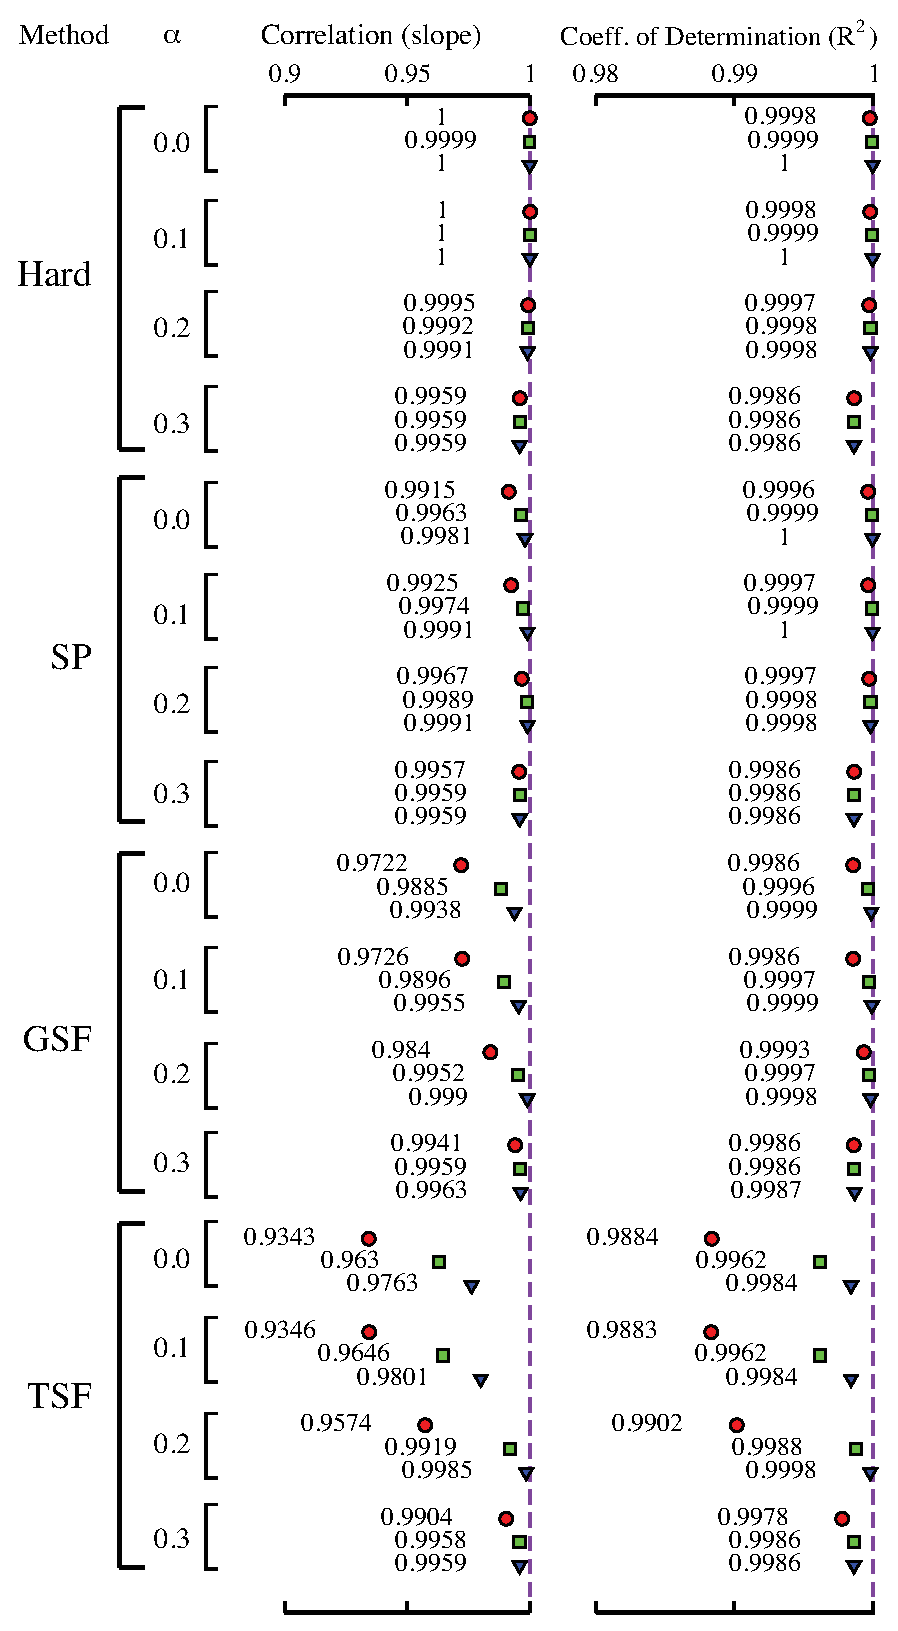
\includegraphics[width=0.6\linewidth]{forcePlot_slopeCorrelation_combined.eps} 
  \caption{Statistical analysis of the quality of the force vector
    magnitudes for the real-space electrostatic methods compared with
    the reference Ewald sum. Results with a value equal to 1 (dashed
    line) indicate force magnitude values indistinguishable from those
    obtained using the multipolar Ewald sum.  Different values of the
    cutoff radius are indicated with different symbols (9~\AA\ =
    circles, 12~\AA\ = squares, and 15~\AA\ = inverted
    triangles).\label{fig:slopeCorr_force}}
\end{figure} 


\begin{figure}
  \centering
  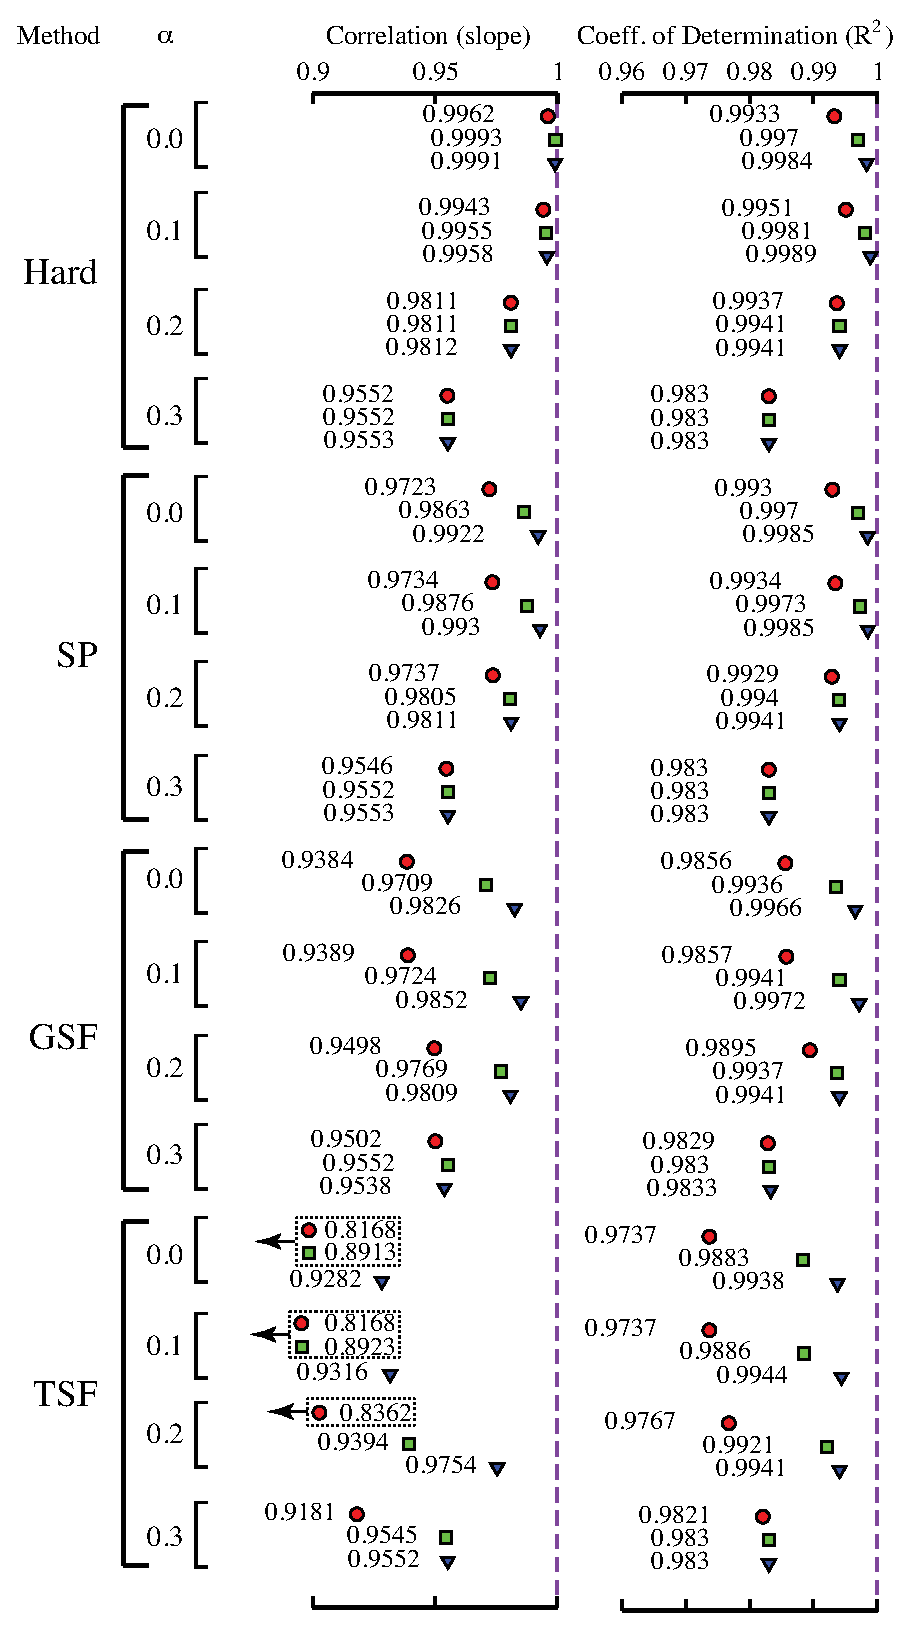
\includegraphics[width=0.6\linewidth]{torquePlot_slopeCorrelation_combined.eps}
  \caption{Statistical analysis of the quality of the torque vector
    magnitudes for the real-space electrostatic methods compared with
    the reference Ewald sum. Results with a value equal to 1 (dashed
    line) indicate force magnitude values indistinguishable from those
    obtained using the multipolar Ewald sum.  Different values of the
    cutoff radius are indicated with different symbols (9~\AA\ =
    circles, 12~\AA\ = squares, and 15~\AA\ = inverted
    triangles).\label{fig:slopeCorr_torque}}
\end{figure}

The torques (Fig. \ref{fig:slopeCorr_torque}) appear to be
significantly influenced by the choice of real-space method.  The
torque expressions have the same distance dependence as the energies,
which are naturally longer-ranged expressions than the inter-site
forces.  Torques are also quite sensitive to orientations of
neighboring molecules, even those that are near the cutoff distance.

The results shows that the torque from the hard cutoff method
reproduces the torques in quite good agreement with the Ewald sum.
The other real-space methods can cause some deviations, but excellent
agreement with the Ewald sum torques is recovered at moderate values
of the damping coefficient ($\alpha \approx 0.2$~\AA$^{-1}$) and cutoff
radius ($r_c \ge 12$~\AA).  The TSF method exhibits only fair agreement
in the slope when compared with the Ewald torques even for larger
cutoff radii.  It appears that the severity of the perturbations in
the TSF method are most in evidence for the torques.

\subsection{Directionality of the force and torque vectors}   

The accurate evaluation of force and torque directions is just as
important for molecular dynamics simulations as the magnitudes of
these quantities. Force and torque vectors for all six systems were
analyzed using Fisher statistics, and the quality of the vector
directionality is shown in terms of circular variance
($\mathrm{Var}(\theta)$) in
Fig. \ref{fig:slopeCorr_circularVariance}. The force and torque
vectors from the new real-space methods exhibit nearly-ideal Fisher
probability distributions (Eq.~\ref{eq:pdf}). Both the hard and SP
cutoff methods exhibit the best vectorial agreement with the Ewald
sum. The force and torque vectors from GSF method also show good
agreement with the Ewald method, which can also be systematically
improved by using moderate damping and a reasonable cutoff radius. For
$\alpha = 0.2$~\AA$^{-1}$ and $r_c = 12$~\AA, we observe
$\mathrm{Var}(\theta) = 0.00206$, which corresponds to a distribution
with 95\% of force vectors within $6.37^\circ$ of the corresponding
Ewald forces. The TSF method produces the poorest agreement with the
Ewald force directions.

Torques are again more perturbed than the forces by the new real-space
methods, but even here the variance is reasonably small.  For the same
method (GSF) with the same parameters ($\alpha = 0.2$~\AA$^{-1}$, $r_c
= 12$~\AA), the circular variance was 0.01415, corresponds to a
distribution which has 95\% of torque vectors are within $16.75^\circ$
of the Ewald results. Again, the direction of the force and torque
vectors can be systematically improved by varying $\alpha$ and $r_c$.

\begin{figure}
  \centering
  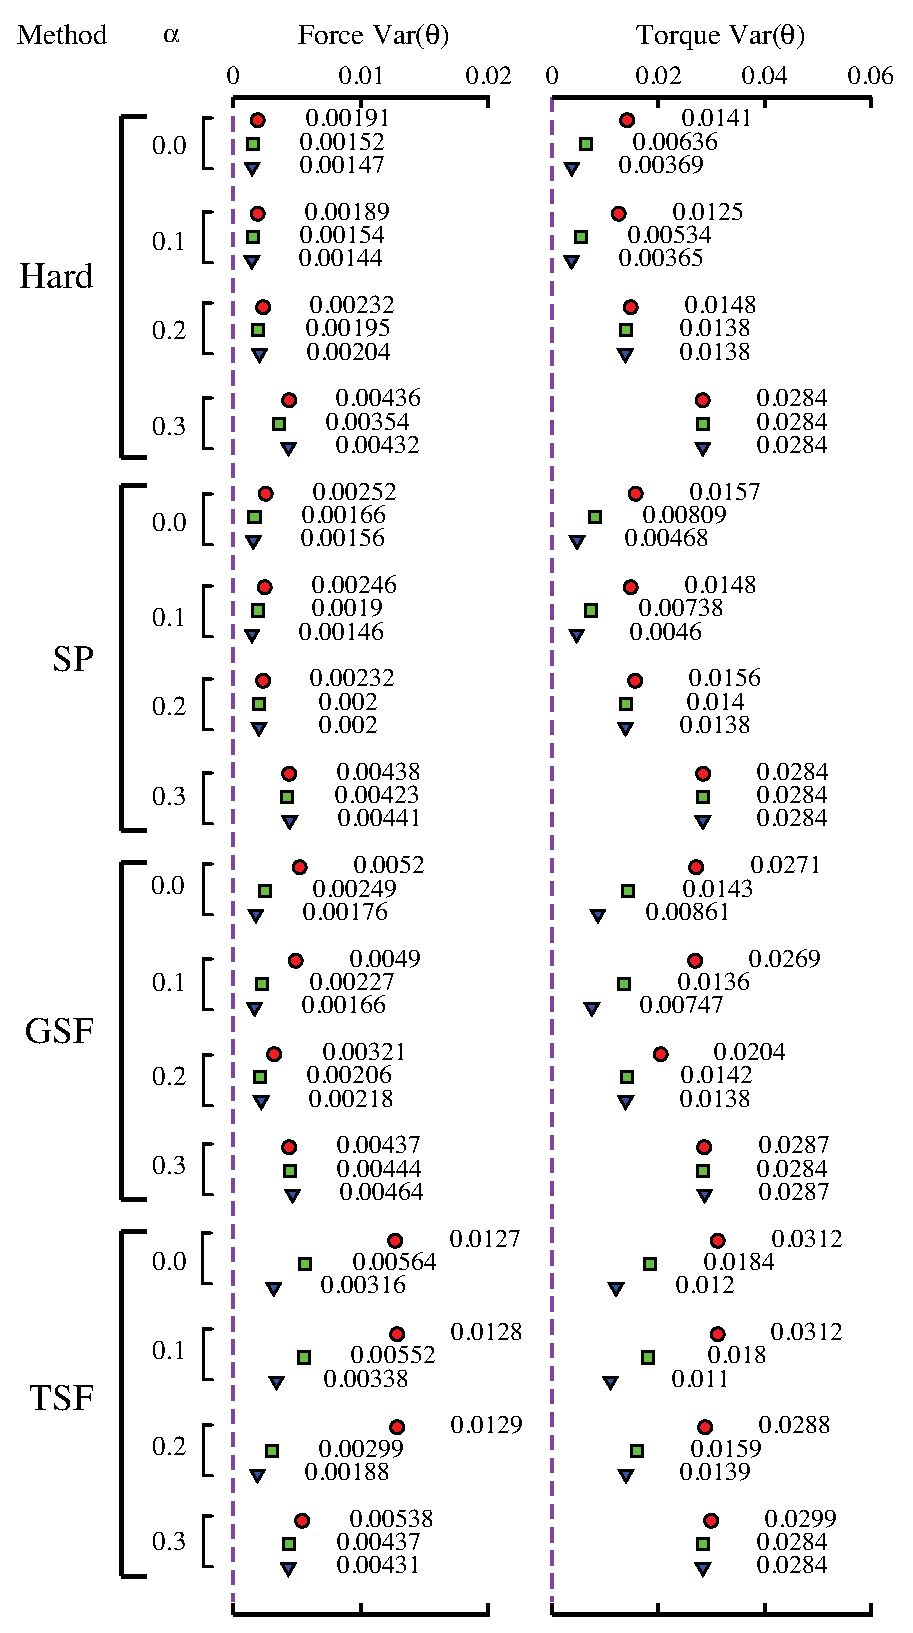
\includegraphics[width=0.65\linewidth]{Variance_forceNtorque_modified.eps}
  \caption{The circular variance of the direction of the force and
    torque vectors obtained from the real-space methods around the
    reference Ewald vectors. A variance equal to 0 (dashed line)
    indicates direction of the force or torque vectors are
    indistinguishable from those obtained from the Ewald sum. Here
    different symbols represent different values of the cutoff radius
    (9~\AA\ = circle, 12~\AA\ = square, 15~\AA\ = inverted triangle)\label{fig:slopeCorr_circularVariance}}
\end{figure}

\subsection{Energy conservation\label{sec:conservation}}

We have tested the conservation of energy one can expect to see with
the new real-space methods using the soft DQ liquid model with a small
fraction of solvated ions. This is a test system which exercises all
orders of multipole-multipole interactions derived in the chapter 2
in this series and provides the most comprehensive test of the new
methods.  A liquid-phase system was created with 2000 liquid-phase
molecules and 48 dissolved ions at a density of 0.98 g cm$^{-3}$ and a
temperature of 300K.  After equilibration in the canonical (NVT)
ensemble using a Nos\'e-Hoover thermostat, six
statistically-independent replicas of this liquid-phase system were
run in the microcanonical (NVE) ensemble under the Ewald, Hard, SP,
GSF, and TSF methods with a cutoff radius of 12~\AA.  The value of the
damping coefficient was also varied from the undamped case ($\alpha =
0$) to a heavily damped case ($\alpha = 0.3$~\AA$^{-1}$) for all of
the real space methods.  A sample was also run using the multipolar
Ewald sum with the same real-space cutoff.

In Fig.~\ref{fig:energyDrift} we show the both the linear drift in
energy over time, $\delta E_1$, and the standard deviation of energy
fluctuations around this drift $\delta E_0$.  Both of the
shifted-force methods (GSF and TSF) provide excellent energy
conservation (drift less than $10^{-5}$ kcal / mol / ns / particle),
while the hard cutoff is essentially unusable for molecular dynamics.
SP provides some benefit over the hard cutoff because the energetic
jumps that happen as particles leave and enter the cutoff sphere are
somewhat reduced, but like the Wolf method for charges, the SP method
would not be as useful for molecular dynamics as either of the
shifted-force methods.

We note that for all tested values of the cutoff radius, the new
real-space methods can provide better energy conservation behavior
than the multipolar Ewald sum, even when relatively large $k$-space
cutoff values are utilized.

\begin{figure}
  \centering
  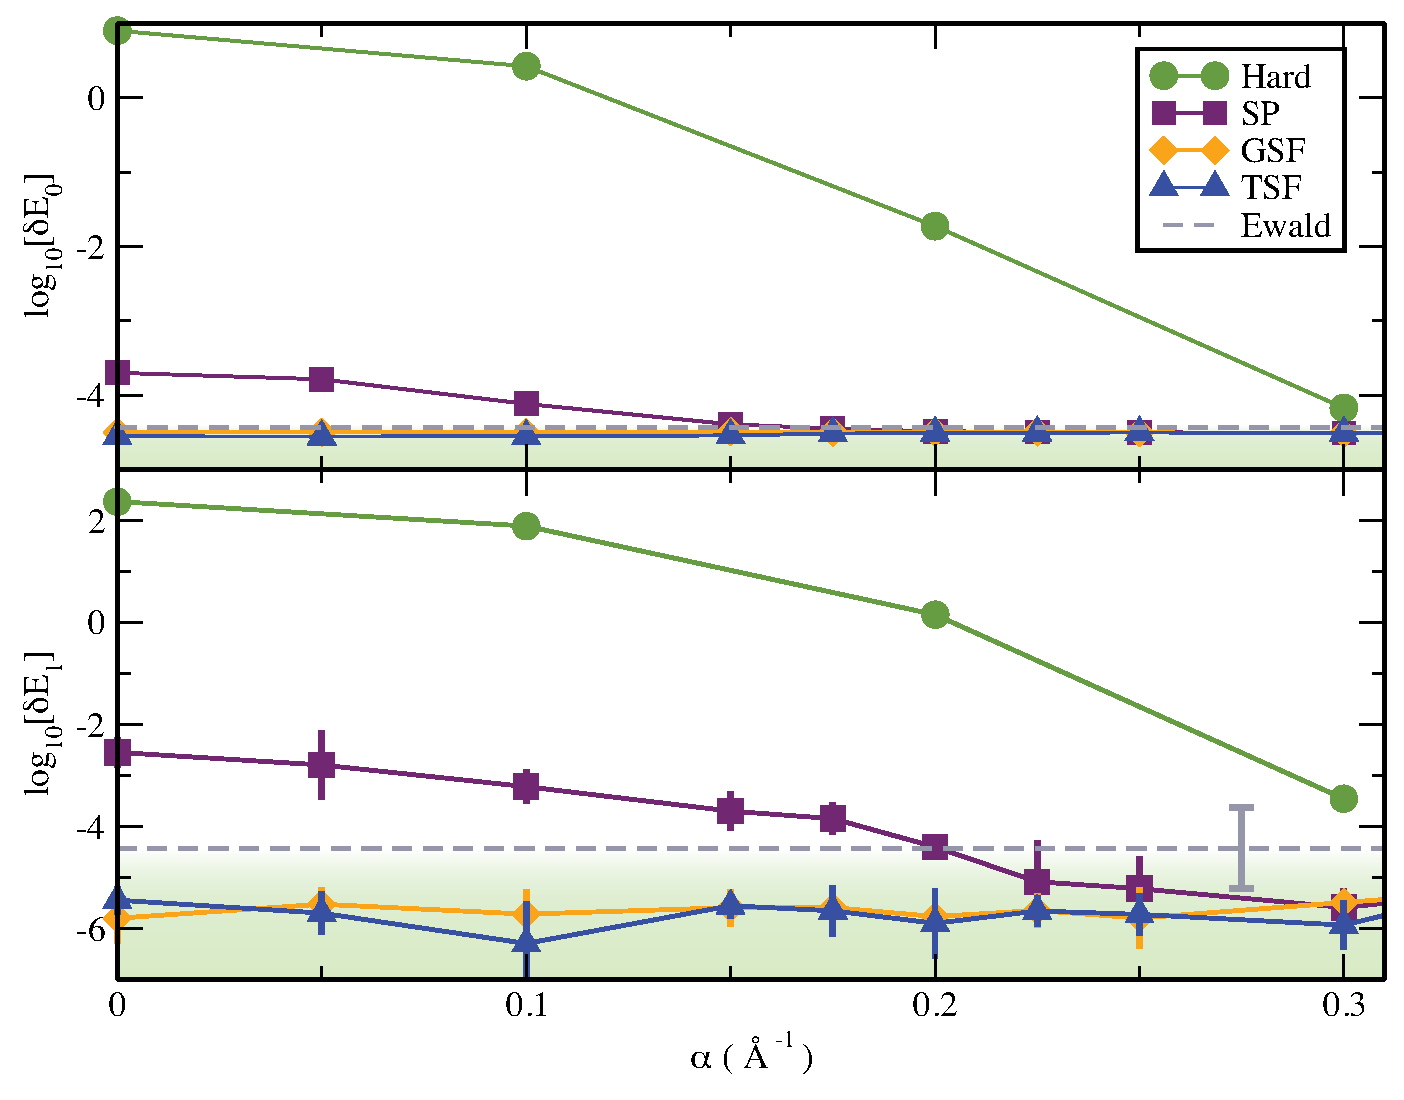
\includegraphics[width=\textwidth]{finalDrift.eps}
  \caption{Energy conservation of the real-space methods for the soft
    DQ liquid / ion system. $\delta \mathrm{E}_1$ is the linear drift
    in energy over time (in kcal/mol/particle/ns) and $\delta
    \mathrm{E}_0$ is the standard deviation of energy fluctuations
    around this drift (in kcal/mol/particle).  Points that appear in
    the green region at the bottom exhibit better energy conservation
    than would be obtained using common parameters for Ewald-based
    electrostatics.\label{fig:energyDrift}}
\end{figure} 
\subsection{Reproduction of Structural \& Dynamical Features\label{sec:structure}}
The most important test of the modified interaction potentials is the
fidelity with which they can reproduce structural features and
dynamical properties in a liquid.  One commonly-utilized measure of
structural ordering is the pair distribution function, $g(r)$, which
measures local density deviations in relation to the bulk density.  In
the electrostatic approaches studied here, the short-range repulsion
from the Lennard-Jones potential is identical for the various
electrostatic methods, and since short range repulsion determines much
of the local liquid ordering, one would not expect to see many
differences in $g(r)$.  Indeed, the pair distributions are essentially
identical for all of the electrostatic methods studied (for each of
the different systems under investigation). 

% An example of this agreement for the soft DQ liquid/ion system is
% shown in Fig. \ref{fig:gofr}.

% \begin{figure}
%   \centering
%   \includegraphics[width=\textwidth]{gofr_ssdqc.eps}
% \caption{The pair distribution functions, $g(r)$, for the SSDQ
%   water/ion system obtained using the different real-space methods are
%   essentially identical with the result from the Ewald
%   treatment.\label{fig:gofr}}
% \end{figure} 

There is a minor over-structuring of the first solvation shell when
using TSF or when overdamping with any of the real-space methods.
With moderate damping, GSF and SP produce pair distributions that are
identical (within numerical noise) to their Ewald counterparts.  The
degree of over-structuring can be measured most easily using the
coordination number,
\begin{equation}
n_C = 4\pi\rho \int_{0}^{a}r^2\text{g}(r)dr,
\end{equation}
where $\rho$ is the number density of the site-site pair interactions,
and $a$ is the radial location of the minima following the first peak
in $g(r)$ ($a = 4.2$~\AA\  for the soft DQ liquid / ion system).  The
coordination number is shown as a function of the damping coefficient
for all of the real space methods in Fig. \ref{fig:Props}.

A more demanding test of modified electrostatics is the average value
of the electrostatic energy $\langle U_\mathrm{elect} \rangle / N$
which is obtained by sampling the liquid-state configurations
experienced by a liquid evolving entirely under the influence of each
of the methods.  In Fig. \ref{fig:Props} we demonstrate how $\langle
U_\mathrm{elect} \rangle / N$ varies with the damping parameter,
$\alpha$, for each of the methods. 

As in the crystals studied in the chapter 2, damping is important
for converging the mean electrostatic energy values, particularly for
the two shifted force methods (GSF and TSF).  A value of $\alpha
\approx 0.2$~\AA$^{-1}$ is sufficient to converge the SP and GSF
energies with a cutoff of 12 \AA, while shorter cutoffs require more
dramatic damping ($\alpha \approx 0.28$~\AA$^{-1}$ for $r_c = 9$~\AA).
Overdamping the real-space electrostatic methods occurs with $\alpha >
0.3$~\AA$^{-1}$, causing the estimate of the electrostatic energy to
drop below the Ewald results.

These ``optimal'' values of the damping coefficient for structural
features are similar to those observed for DSF electrostatics for
purely point-charge systems, and the range $\alpha= 0.175 \rightarrow
0.225$~\AA$^{-1}$ for $r_c = 12$~\AA\ appears to be an excellent
compromise for mixed charge/multipolar systems.

To test the fidelity of the electrostatic methods at reproducing
\textit{dynamics} in a multipolar liquid, it is also useful to look at
transport properties, particularly the diffusion constant,
\begin{equation}
D = \lim_{t \rightarrow \infty} \frac{1}{6 t} \langle \left|
  \mathbf{r}(t) -\mathbf{r}(0) \right|^2 \rangle
\label{eq:diff}
\end{equation}
which measures long-time behavior and is sensitive to the forces on
the multipoles. The self-diffusion constants (D) were calculated from
linear fits to the long-time portion of the mean square displacement,
$\langle r^{2}(t) \rangle$.\cite{Allen89} In Fig. \ref{fig:Props} we
demonstrate how the diffusion constant depends on the choice of
real-space methods and the damping coefficient.  Both the SP and GSF
methods can obtain excellent agreement with Ewald again using moderate
damping.

In addition to translational diffusion, orientational relaxation times
were calculated for comparisons with the Ewald simulations and with
experiments. These values were determined by calculating the
orientational time correlation function,
\begin{equation}
C_l^\gamma(t) = \left\langle P_l\left[\hat{\mathbf{A}}_\gamma(t)
                \cdot\hat{\mathbf{A}}_\gamma(0)\right]\right\rangle,
\label{eq:OrientCorr}
\end{equation}
from the same 350 ps microcanonical trajectories that were used for
translational diffusion.  Here, $P_l$ is the Legendre polynomial of
order $l$ and $\hat{\mathbf{A}}_\gamma$ is the unit vector for body
axis $\gamma$.  The reference frame used for our sample dipolar
systems has the $z$-axis running along the dipoles, and for the soft
DQ liquid model, the $y$-axis connects the two implied hydrogen-like
positions.  From the orientation autocorrelation functions, we can
obtain time constants for rotational relaxation either by fitting to a
multi-exponential model for the orientational relaxation, or by
integrating the correlation functions.

In a good model for water, the orientational decay times would be
comparable to water orientational relaxation times from nuclear
magnetic resonance (NMR). The relaxation constant obtained from
$C_2^y(t)$ is normally of experimental interest because it describes
the relaxation of the principle axis connecting the hydrogen
atoms. Thus, $C_2^y(t)$ can be compared to the intermolecular portion
of the dipole-dipole relaxation from a proton NMR signal and can
provide an estimate of the NMR relaxation time constant.\cite{Impey82}
In Fig. \ref{fig:Props} we compare the $\tau_2^y$ and $\tau_2^z$
values for the various real-space methods over a range of different
damping coefficients.  The rotational relaxation for the $z$ axis
primarily probes the torques on the dipoles, while the relaxation for
the $y$ axis is sensitive primarily to the quadrupolar torques.

\begin{figure}
  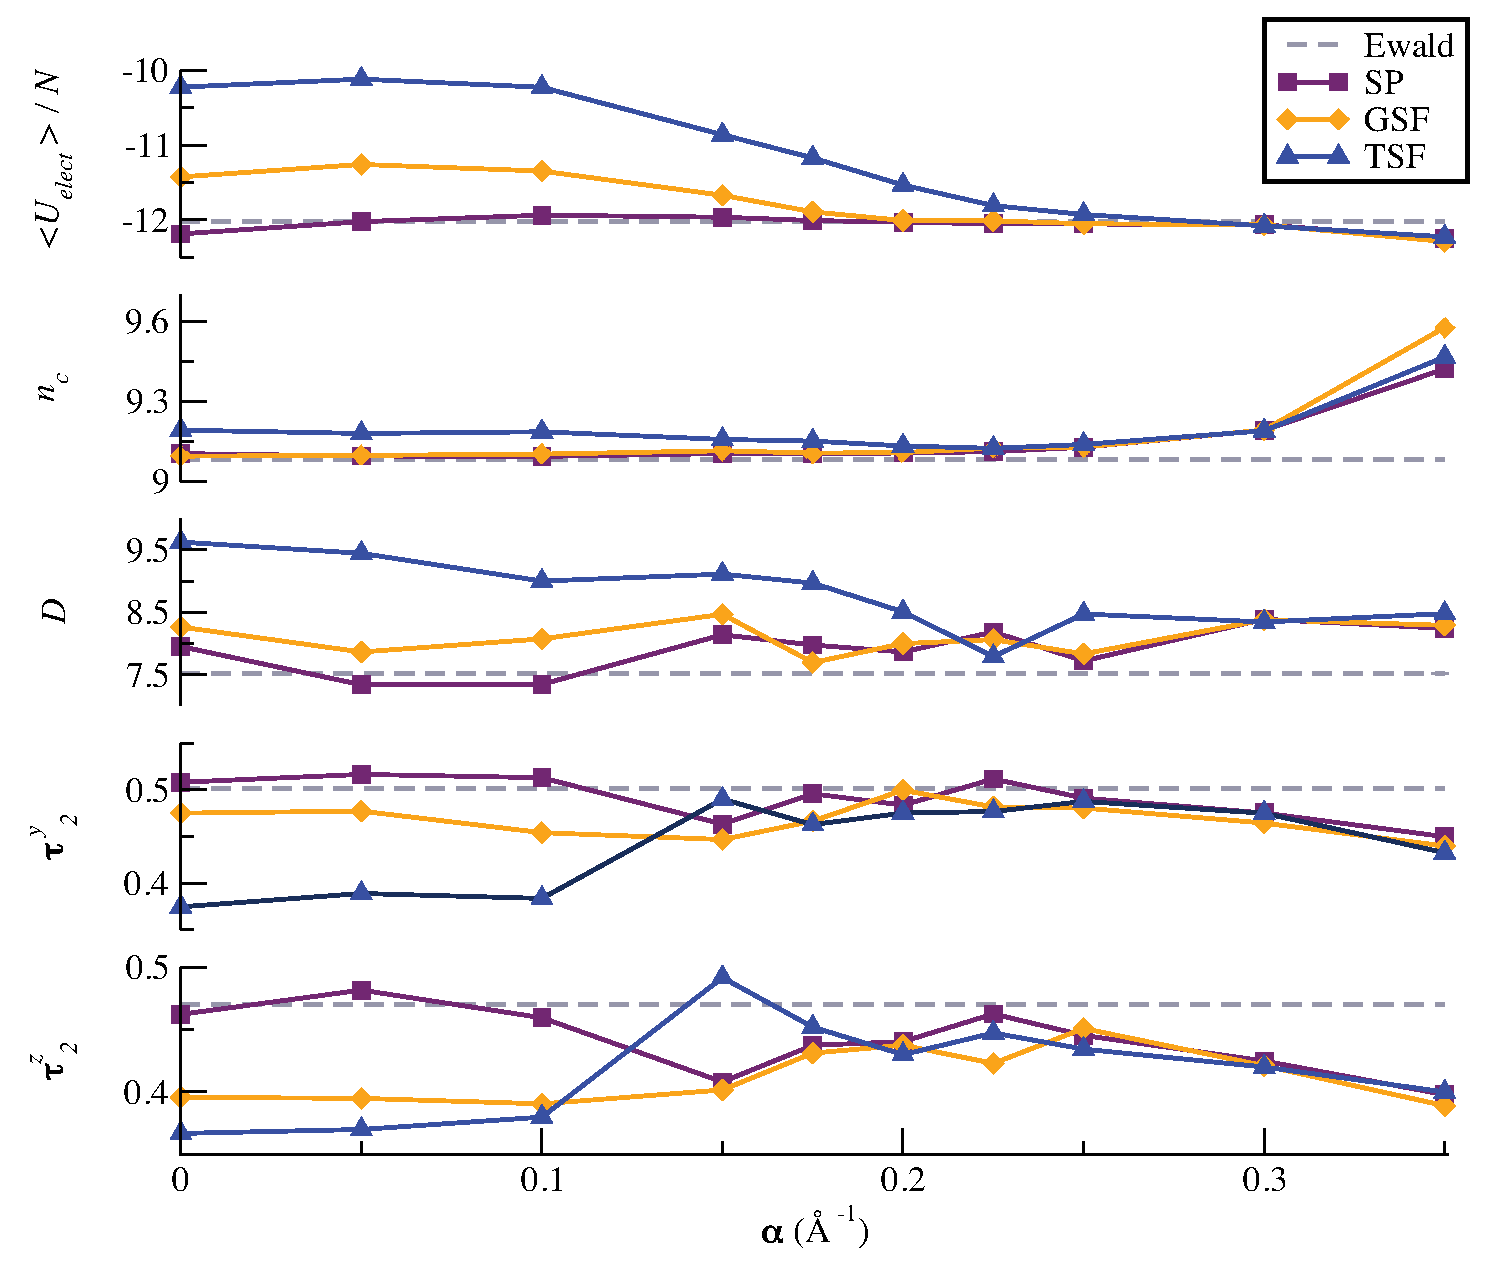
\includegraphics[width=\textwidth]{properties.eps}
  \caption{Comparison of the structural and dynamic properties for the
    combined multipolar liquid (soft DQ liquid + ions) for all of the
    real-space methods with $r_c = 12$~\AA. Electrostatic energies,
    $\langle U_\mathrm{elect} \rangle / N$ (in kcal / mol),
    coordination numbers, $n_C$, diffusion constants (in $10^{-5}
    \mathrm{cm}^2\mathrm{s}^{-1}$), and rotational correlation times
    (in ps) all show excellent agreement with Ewald results for
    damping coefficients in the range $\alpha= 0.175 \rightarrow
    0.225$~\AA$^{-1}$. \label{fig:Props}}
\end{figure}

In Fig. \ref{fig:Props} it appears that values for $D$, $\tau_2^y$,
and $\tau_2^z$ using the Ewald sum are reproduced with excellent
fidelity by the GSF and SP methods.  All of the real space methods can
be \textit{overdamped}, which reduces the effective range of multipole
interactions, causing structural and dynamical changes from the
correct behavior.  Because overdamping weakens orientational
preferences between adjacent molecules, it manifests as too-rapid
orientational decay coupled with faster diffusion and
over-coordination of the liquid.  Underdamping is less problematic for
the SP and GSF methods, as their structural and dynamical properties
still reproduce the Ewald results even in the completely undamped
($\alpha = 0$) case.  An optimal range for the electrostatic damping
parameter appears to be $\alpha= 0.175 \rightarrow 0.225$~\AA$^{-1}$
for $r_c = 12$~\AA, which similar to the optimal range found for the
damped shifted force potential for point charges.\cite{Gezelter06}

\section{Summary}
In the chapter 2, we generalized the
charge-neutralized electrostatic energy originally developed by Wolf
\textit{et al.}\cite{Wolf99} to multipole-multipole interactions
up to quadrupolar order.  The SP method is essentially a
multipole-capable version of the Wolf model.  The SP method for
multipoles provides excellent agreement with Ewald-derived energies,
forces and torques, and is suitable for Monte Carlo simulations,
although the forces and torques retain discontinuities at the cutoff
distance that prevents its use in molecular dynamics.

We also developed two natural extensions of the damped shifted-force
(DSF) model originally proposed by Zahn {\it et al.} and extended by
Fennell and Gezelter.\cite{Zahn02, Gezelter06} The GSF and TSF
approaches provide smooth truncation of energies, forces, and torques
at the real-space cutoff, and both converge to DSF electrostatics for
point-charge interactions.  The TSF model is based on a high-order
truncated Taylor expansion which can be relatively perturbative inside
the cutoff sphere.  The GSF model takes the gradient from an images of
the interacting multipole that has been projected onto the cutoff
sphere to derive shifted force and torque expressions, and is a
significantly more gentle approach.

The GSF method produces quantitative agreement with Ewald energies,
forces, and torques.  It also performs well in conserving energy in MD
simulations.  The Taylor-shifted (TSF) model provides smooth dynamics,
but these take place on a potential energy surface that is
significantly perturbed from Ewald-based electrostatics.  Because it
performs relatively poorly compared with GSF, it may seem odd that
that the TSF model was included in this work.  However, the functional
forms derived for the SP and GSF methods depend on the separation of
orientational contributions that were made visible by the Taylor
series of the electrostatic kernel at the cutoff radius. The TSF
method also has the unique property that a large number of derivatives
can be made to vanish at the cutoff radius.  This property has proven
useful in past treatments of the corrections to the Clausius-Mossotti
fluctuation formula for dielectric constants.\cite{Izvekov08}

Reproduction of both structural and dynamical features in the liquid
systems is remarkably good for both the SP and GSF models.  Pair
distribution functions are essentially equivalent to the same
functions produced using Ewald-based electrostatics, and with moderate
damping, a structural feature that directly probes the electrostatic
interaction (e.g. the mean electrostatic potential energy) can also be
made quantitative.  Dynamical features are sensitive probes of the
forces and torques produced by these methods, and even though the
smooth behavior of forces is produced by perturbing the overall
potential, the diffusion constants and orientational correlation times
are quite close to the Ewald-based results.

The only cases we have found where the new GSF and SP real-space
methods can be problematic are those which retain a bulk dipole moment
at large distances (e.g. the $Z_1$ dipolar lattice).  In ferroelectric
materials, uniform weighting of the orientational contributions can be
important for converging the total energy.  In these cases, the
damping function which causes the non-uniform weighting can be
replaced by the bare electrostatic kernel, and the energies return to
the expected converged values.

Based on the results of this work, we can conclude that the GSF method
is a suitable and efficient replacement for the Ewald sum for
evaluating electrostatic interactions in modern MD simulations, and
the SP method would be an excellent choice for Monte Carlo
simulations where smooth forces and energy conservation are not
important.  Both the SP and GSF methods retain excellent fidelity to
the Ewald energies, forces and torques.  Additionally, the energy
drift and fluctuations from the GSF electrostatics are significantly
better than a multipolar Ewald sum for finite-sized reciprocal spaces,
and physical properties are reproduced accurately.

As in all purely pairwise cutoff methods, the SP, GSF and TSF methods
are expected to scale approximately {\it linearly} with system size,
and are easily parallelizable.  This should result in substantial
reductions in the computational cost of performing large simulations.
With the proper use of pre-computation and spline interpolation of the
radial functions, the real-space methods are essentially the same cost
as a simple real-space cutoff.  They require no Fourier transforms or
$k$-space sums, and guarantee the smooth handling of energies, forces,
and torques as multipoles cross the real-space cutoff boundary.

We are not suggesting that there is any flaw with the Ewald sum; in
fact, it is the standard by which the SP, GSF, and TSF methods have
been judged in this work.  However, these results provide evidence
that in the typical simulations performed today, the Ewald summation
may no longer be required to obtain the level of accuracy most
researchers have come to expect.



% % uncomment the following lines,
% if using chapter-wise bibliography
%
% \bibliographystyle{ndnatbib}
% \bibliography{example}


% Chapter 4

%
% Modified by Megan Patnott
% Last Change: Jan 18, 2013
%
%%%%%%%%%%%%%%%%%%%%%%%%%%%%%%%%%%%%%%%%%%%%%%%%%%%%%%%%%%%%%%%%%%%%%%%%
%
% Modified by Sameer Vijay
% Last Change: Wed Jul 27 2005 13:00 CEST
%
%%%%%%%%%%%%%%%%%%%%%%%%%%%%%%%%%%%%%%%%%%%%%%%%%%%%%%%%%%%%%%%%%%%%%%%%
%
% Sample Notre Dame Thesis/Dissertation
% Using Donald Peterson's ndthesis classfile
%
% Written by Jeff Squyres and Don Peterson
%
% Provided by the Information Technology Committee of
%   the Graduate Student Union
%   http://www.gsu.nd.edu/
%
% Nothing in this document is serious except the format.  :-)
%
% If you have any suggestions, comments, questions, please send e-mail
% to: ndthesis@gsu.nd.edu
%
%%%%%%%%%%%%%%%%%%%%%%%%%%%%%%%%%%%%%%%%%%%%%%%%%%%%%%%%%%%%%%%%%%%%%%%%

%
% Chapter 4
%


\chapter{DIELECTRIC PROPERTIES}
\label{chap:dielectric}
In the previous chapter, we have derived various physical properties considering SP, GSF, and TSF methods and tested result against the multipolar Ewald method. In this chapter, we discuss fluctuation, perturbation, and potential of mean force (PMF) methods for calculating the dielectric properties of the dipolar and quadrupolar fluids using newly developed real space methods. Since the dielectric constant is a macroscopic property, the interactions of a molecule with the rest of the molecules of the system are important. Our newly developed real space methods utilize a cutoff radius which reduces the number of interactions calculated in the system. Hence, the formula for the dielectric constant should be modified accordingly. Therefore to get correct dielectric properties using the result obtained from the simulation, we need to evaluate correction factor for each real-space methods separately. In this chapter, we have also calculated the correction factors for each real-space methods and tabulated for both dipolar and quadrupolar fluids.

\section{Introduction}
One of the most difficult tests of any new electrostatic method is the
fidelity with which that method can reproduce the bulk-phase
polarizability or equivalently, the dielectric properties of a
fluid. Before the advent of computer simulations, Kirkwood and Onsager
developed fluctuation formulae for the dielectric properties of
dipolar fluids.\cite{Kirkwood39,Onsagar36}
Of particular interest is the static dielectric constant, $\epsilon$.
Using the Ewald sum under tin-foil boundary conditions, $\epsilon$ can
be calculated for systems of non-polarizable substances via
\begin{equation}
\epsilon = 1 + \frac{\langle M^2\rangle}{3\epsilon_0k_\textrm{B}TV},
\label{eq:staticDielectric}
\end{equation}
where $\epsilon_0$ is the permittivity of free space and
$\langle M^2\rangle$ is the fluctuation of the system dipole
moment.\cite{Allen89} The numerator in the fractional term in
equation (\ref{eq:staticDielectric}) is identical to the quantity
calculated in the finite-system Kirkwood $g$ factor ($G_k$):
\begin{equation}
G_k = \frac{\langle M^2\rangle}{N\mu^2},
\label{eq:KirkwoodFactor}
\end{equation}
where $\mu$ is the dipole moment of a single molecule of the
homogeneous system.\cite{NeumannI83,NeumannII83,Neumann84,Neumann85} The
fluctuation term in both equation (\ref{eq:staticDielectric}) and
(\ref{eq:KirkwoodFactor}) is calculated as follows,
\begin{equation}
\begin{split}
\langle M^2\rangle &= \langle\bm{M}\cdot\bm{M}\rangle 
                        - \langle\bm{M}\rangle\cdot\langle\bm{M}\rangle \\
                   &= \langle M_x^2+M_y^2+M_z^2\rangle
                        - (\langle M_x\rangle^2 + \langle M_x\rangle^2 
                                + \langle M_x\rangle^2).        
\end{split}
\label{eq:fluctBoxDipole}
\end{equation}
This fluctuation term can be accumulated during a simulation; however,
it converges rather slowly, thus requiring multi-nanosecond simulation
times.\cite{Horn04} In the case of tin-foil boundary conditions, the
dielectric/surface term of the Ewald summation is equal to zero.

Similar formulae were developed by Logan \textit{et al.} for the bulk
polarizability of quadrupolar fluids.\cite{LoganI81,LoganII82,LoganIII82}
In modern simulations, bulk materials are usually treated using
periodic replicas of small regions, and this level of approximation
requires corrections to the fluctuation formulae that were derived for
the bulk fluids. In 1983 Neumann proposed a general formula for
evaluating dielectric properties of dipolar fluids using real-space
cutoff methods.\cite{NeumannI83} Steinhauser and Neumann used this
formula to evaluate the corrected dielectric constant for the
Stockmayer fluid using two different methods: Ewald-Kornfield (EK) and
reaction field (RF) methods.\cite{NeumannII83}

Zahn \textit{et al.}\cite{Zahn02} utilized this approach and evaluated
the correction factor for using damped shifted charge-charge
kernel. This was later generalized by Izvekov \textit{et
  al.},\cite{Izvekov08} who that the expression for the
dielectric constant reduces to widely-used \textit{conducting
  boundary} formula for real-space cutoff methods that have first
derivatives that vanish at the cutoff sphere.

In quadrupolar fluids, the relationship between quadrupolar
susceptibility and the dielectric constant is not as straightforward
as in the dipolar case. The dielectric constant depends on the
geometry of the external field perturbation.\cite{Ernst92} Significant
efforts have been made to increase our understanding the dielectric
properties of these fluids,\cite{JeonI03,JeonII03,Chitanvis96}
although a correction formula for different real-space methods has not
yet been developed.

In this paper we derive general formulae for calculating the
dielectric properties of quadrupolar fluids. We also evaluate the
correction factor for SP, GSF, and TSF methods for both dipolar and
quadrupolar fluids interacting via point charges, point dipoles or
through quadrupole-quadrupole interactions.

We have also calculated the screening behavior for two ions immersed
in a quadrupolar fluid to estimate the dielectric screening from the
quadrupolar susceptibility.  We have used three different methods to
compare our results with computer simulations:
\begin{enumerate}
\item responses of the fluid to external perturbations,
\item fluctuations of box multipole moments, and
\item potentials of mean force between solvated ions,
\end{enumerate}

In the external field perturbation, the net polarization of the system
is observed as a linear response of the applied field perturbation,
where proportionality constant is determined by the electrostatic
interaction between the electrostatic multipoles at a given
temperature. The fluctuation formula observes the time average
fluctuation of the multipolar moment as a function of temperature. The
average fluctuation value of the system is determined by the
multipole-multipole interactions between molecules at a given
temperature. Since the expression of the electrostatic interaction
energy, force, and torque in the real space electrostatic methods are
different from their original definition, both fluctuation and
external field perturbation formula should also be modified
accordingly. The potential of mean force method calculates dielectric
constant or screening factor from the potential energy between ions before and after dielectric material is introduced. All of these different methods for
calculating dielectric properties will be discussed in detail in the
following sections: \ref{subsec:perturbation},\ref{subsec:fluctuation}, and \ref{sec:PMF}.

\section{Boltzmann average for orientational polarization}
The dielectric properties of the system is mainly arise from two different ways: i) the applied field distort the charge distributions so it produces an induced multipolar moment in each molecule; and ii) the applied field tends to line up originally randomly oriented molecular moment towards the direction of the applied field. In this study, we basically focus on the orientational contribution in the dielectric properties. If we consider a system of molecules in the presence of external field perturbation, the perturbation experienced by any molecule will not be only due to external field or field gradient but also due to the field or field gradient produced by the all other molecules in the system. In the following subsections \ref{subsec:boltzAverage-Dipole} and \ref{subsec:boltzAverage-Quad}, we will discuss about the molecular polarization only due to external field perturbation. The contribution of the field or field gradient due to all other molecules will be taken into account while calculating correction factor in the section \ref{sec:corrFactor}.

\subsection{Dipole}
\label{subsec:boltzAverage-Dipole}
Consider a system of molecules, each with permanent dipole moment
$p_o$. In the absense of external field, thermal agitation orients the
dipoles randomly, reducing the system moment to zero.  External fields
will tend to line up the dipoles in the direction of applied field.
Here we have considered net field from all other molecules is
considered to be zero.  Therefore the total Hamiltonian of each
molecule is,\cite{Jackson98}
\begin{equation}
H = H_o - \bf{p_o} .\bf{E},
\end{equation}
where $H_o$ is a function of the internal coordinates of the molecule.
The Boltzmann average of the dipole moment is given by,
\begin{equation}
\braket{p_{mol}} = \frac{\displaystyle\int d\Omega\; p_o\; cos\theta\;  e^{\frac{p_oE\; cos\theta}{k_B T}}}{\displaystyle\int d\Omega\; e^{\frac{p_oE\;cos\theta}{k_B T}}},
\end{equation}
where $\bf{E}$ is selected along z-axis. If we consider that the
applied field is small, \textit{i.e.} $\frac{p_oE\; cos\theta}{k_B T} << 1$, 
\begin{equation}
\braket{p_{mol}}  \approx \frac{1}{3}\frac{{p_o}^2}{k_B T}E,
\end{equation}
where $ \alpha_p = \frac{1}{3}\frac{{p_o}^2}{k_B T}$ is a molecular
polarizability. The orientational polarization depends inversely on
the temperature and applied field must overcome the thermal agitation.

\subsection{Quadrupole}
\label{subsec:boltzAverage-Quad}
Consider a system of molecules with permanent quadrupole moment $q_{\alpha\beta} $. The average quadrupole moment at temperature T in the presence of uniform applied field gradient is given by,\cite{AduGyamfi78, AduGyamfi81}
\begin{equation}
\braket{q_{\alpha\beta}} \;=\; \frac{\displaystyle\int d\Omega\; e^{-\frac{H}{k_B T}}q_{\alpha\beta}}{\displaystyle\int d\Omega\; e^{-\frac{H}{k_B T}}} \;=\; \frac{\displaystyle\int d\Omega\; e^{\frac{q_{\mu\nu}\;\partial_\nu E_\mu}{k_B T}}q_{\alpha\beta}}{\displaystyle\int d\Omega\; e^{\frac{q_{\mu\nu}\;\partial_\nu E_\mu}{k_B T}}},
\label{boltzQuad}
\end{equation}
where $\int d\Omega = \int_0^{2\pi} \int_0^\pi \int_0^{2\pi}
sin\theta\; d\theta\ d\phi\ d\psi$ is the integration over Euler
angles, $ H = H_o -q_{\mu\nu}\;\partial_\nu E_\mu $ is the energy of
a quadrupole in the gradient of the  
applied field and $ H_o$ is a function of internal coordinates of the molecule. The energy and quadrupole moment can be transformed into body frame using following relation, 
\begin{equation}
\begin{split}
&q_{\alpha\beta} = \eta_{\alpha\alpha'}\;\eta_{\beta\beta'}\;{q}^* _{\alpha'\beta'} \\
&H = H_o - q:\vec{\nabla}\vec{E} = H_o - q_{\mu\nu}\;\partial_\nu E_\mu = H_o -\eta_{\mu\mu'}\;\eta_{\nu\nu'}\;{q}^*_{\mu'\nu'}\;\partial_\nu E_\mu.
\end{split}
\label{energyQuad}
\end{equation}
Here the starred tensors are the components in the body fixed
frame. Substituting equation (\ref{energyQuad}) in the equation (\ref{boltzQuad})
and taking linear terms in the expansion we get,
\begin{equation}
\braket{q_{\alpha\beta}} = \frac{ \int d\Omega \left(1 + \frac{\eta_{\mu\mu'}\;\eta_{\nu\nu'}\;{q}^*_{\mu'\nu'}\;\partial_\nu E_\mu }{k_B T}\right)q_{\alpha\beta}}{ \int d\Omega \left(1 + \frac{\eta_{\mu\mu'}\;\eta_{\nu\nu'}\;{q}^*_{\mu'\nu'}\;\partial_\nu E_\mu }{k_B T}\right)},
\end{equation}
where $\eta_{\alpha\alpha'}$ is the inverse of the rotation matrix that transforms
the body fixed co-ordinates to the space co-ordinates,
\[\eta_{\alpha\alpha'} 
= \left(\begin{array}{ccc}
cos\phi\; cos\psi - cos\theta\; sin\phi\; sin\psi & -cos\theta\; cos\psi\; sin\phi - cos\phi\; sin\psi & sin\theta\; sin\phi \\
cos\psi\; sin\phi + cos\theta\; cos\phi \; sin\psi & cos\theta\; cos\phi\; cos\psi - sin\phi\; sin\psi & -cos\phi\; sin\theta \\
sin\theta\; sin\psi & -cos\psi\; sin\theta & cos\theta
\end{array} \right).\]
Integration of 1st and 2nd terms in the denominator gives $8 \pi^2$
and $8 \pi^2 /3\;\vec{\nabla}.\vec{E}\; Tr(q^*) $ respectively. The
second term vanishes for charge free space
(i.e. $\vec{\nabla}.\vec{E} \; = \; 0)$. Similarly integration of the
1st term in the numerator produces
$8 \pi^2 /3\; Tr(q^*)\delta_{\alpha\beta}$ and the 2nd term produces
$8 \pi^2 /15k_B T (3{q}^*_{\alpha'\beta'}{q}^*_{\beta'\alpha'} -
{q}^*_{\alpha'\alpha'}{q}^*_{\beta'\beta'})\partial_\alpha E_\beta$,
if $\vec{\nabla}.\vec{E} \; = \; 0$,
$ \partial_\alpha E_\beta = \partial_\beta E_\alpha$ and
${q}^*_{\alpha'\beta'}= {q}^*_{\beta'\alpha'}$. Therefore the
Boltzmann average of a quadrupole moment can be written as,

\begin{equation}
\braket{q_{\alpha\beta}}\; = \; \frac{1}{3} Tr(q^*)\;\delta_{\alpha\beta} + \frac{{\bar{q_o}}^2}{15k_BT}\;\partial_\alpha E_\beta,
\end{equation}
where $ \alpha_q = \frac{{\bar{q_o}}^2}{15k_BT} $ is a molecular quadrupolarizablity  and  ${\bar{q_o}}^2=
3{q}^*_{\alpha'\beta'}{q}^*_{\beta'\alpha'}-{q}^*_{\alpha'\alpha'}{q}^*_{\beta'\beta'}$ is a square of the net quadrupole moment of a molecule. 

\section{Macroscopic Polarizability}
\label{sec:MacPolarizablity}

If we consider a system of dipolar or quadrupolar fluid in the external field perturbation, the net polarization of the system will still be proportional to the applied field perturbation.\cite{Chitanvis96, Stern-Feller03, SalvchovI14, SalvchovII14} In simulation the net polarization of the system is determined by the interaction of molecule with all other molecules as well as external field perturbation. Therefore the macroscopic polarizablity obtained from the simulation always varies with nature of real-space electrostatic interaction methods implemented in the simulation. To determine a susceptibility or dielectric constant of the material (which is a actual physical property of the dipolar or quadrupolar fluid) from the macroscopic polarizablity, we need to incorporate the interaction between molecules which has been discussed in detail in section \ref{sec:corrFactor}. In this section we discuss about the two different methods of calculating macroscopic polarizablity for both dipolar and quadrupolar fluid. 

\subsection{External field perturbation}
\label{subsec:perturbation}
In the presence of uniform electric field $\textbf{E}^o$, a system of dipolar  molecules polarizes along the direction of the applied field (or field gradient). Therefore the net dipolar polarization $ \textbf{P}$ of the system is,
\begin{equation}
\textbf{P} = \epsilon_o \alpha_{D}\; \textbf{E}^o. 
\label{pertDipole}
\end{equation} 
The constant $\alpha_D$ is a macroscopic polarizability, which is a property of the dipolar fluid in a given density and temperature.

Similarly, in the presence of external field gradient the system of quadrupolar molecule polarizes along the direction of applied field gradient therefore the net quadrupolar polarization of the system can be given by,
\begin{equation}
\begin{split}
& {Q}_{\alpha\beta} = \frac{1}{3}\; Tr({Q})\; \delta_{\alpha\beta} +  \epsilon_o\; \alpha_Q \; \partial_{\alpha} E^o_{\beta} 
\\ & or \\
& \frac{1}{3}\;\Theta_{\alpha\beta} =  \epsilon_o\; \alpha_Q \; \partial_{\alpha} E^o_{\beta} 
\end{split}
\label{pertQuad}
\end{equation} 
where $Q_{\alpha\beta}$ is a tensor component of the traced quadrupolar moment of the system, $ \alpha_Q$ is a macroscopic quadrupolarizability has a dimension of $length^{-2}$, and $\Theta_{\alpha\beta} = 3Q_{\alpha\beta}-Tr(Q) $ is the traceless component of the quadrupole moment.    

\subsection{Fluctuation formula}
\label{subsec:fluctuation}
For a system of molecules with net dipolar moment $\bf{M}$ at thermal equilibrium of temperature T in the presence of applied field $\bf{E}^o$, the average dipolar polarization can be expressed in terms of fluctuation of the net dipole moment as below,\cite{Stern03}
\begin{equation}
\braket{\bf{P}} = \epsilon_o \frac{\braket{\bf{M}^2}-{\braket{\bf{M}}}^2}{3 \epsilon_o V k_B T}\bf{E}^o
\label{flucDipole}
\end{equation}
This is similar to the formula for boltzmann average of single dipolar molecule in the subsection \ref{subsec:boltzAverage-Dipole}. Here $\braket{\bf{P}}$ is average polarization and $ \braket{\textbf{M}^2}-{\braket{\textbf{M}}}^2$ is the net dipole fluctuation at temperature T. For the limiting case $\textbf{E}^o \rightarrow 0 $, ensemble average of both net dipole moment $\braket{\textbf{M}}$ and dipolar polarization $\braket{\bf{P}}$ tends to vanish but $\braket{\bf{M}^2}$ will still be non-zero. The dipolar macroscopic polarizability can be written as,
\begin{equation}
\alpha_D = \frac{\braket{\bf{M}^2}-{\braket{\bf{M}}}^2}{3 \epsilon_o V k_B T}
\end{equation}
This is a macroscopic property of dipolar material which is true even if applied field $ \textbf{E}^o \rightarrow 0 $.  

Analogous formula can also be written for a system with quadrupolar molecules,
\begin{equation}
\braket{Q_{\alpha\beta}} = \frac{1}{3} Tr(\textbf{Q})\; \delta_{\alpha\beta} + \epsilon_o \frac{\braket{\textbf{Q}^2}-{\braket{\textbf{Q}}}^2}{15 \epsilon_o V k_B T}{\partial_\alpha E^o_\beta}
\label{flucQuad}
\end{equation}
where $Q_{\alpha\beta}$ is a component of system quadrupole moment,  $\bf{Q}$ is net quadrupolar moment which can be expressed as $\textbf{Q}^2 =3Q_{\alpha\beta}Q_{\alpha\beta}-(Tr\textbf{Q})^2 $. The macroscopic quadrupolarizability is given by,
\begin{equation}
\alpha_Q = \frac{\braket{\textbf{Q}^2}-{\braket{\textbf{Q}}}^2}{15 \epsilon_o V k_B T}
\label{propConstQuad}
\end{equation}

\section{Potential of mean force}
In this method, we will measure the interaction between a positive and negative charge at varying distances after introducing a dipolar (or quadrupolar) material between them. The potential of mean force (PMF) between two ions in a liquid is obtained by constraining their distance and measuring the mean constraint force required to hold them at a fixed distance $r.$ The PMF  is obtained from a sequence of simulations can be expressed as \cite{Wilfred07},
\begin{equation}
w(r) = \int_{r_o}^{r}\braket{\frac{\partial f}{\partial r'}}dr' + 2kT \log(r/r_o) + w(r_o),
\label{eq:pmf}
\end{equation}
where $\braket{\partial f/\partial r'}$ is the mean constraint force, $2kT \log(r/r_o)$ is the Fixman factor, and $r_o$ is the reference position. The potential energy between two charges at separation $r$ is given by,
\begin{equation}
w(r) = \frac{1}{4\pi\epsilon}\frac{q_1q_2}{r},
\end{equation}
where $\epsilon$ is the dielectric constant for the fluid.

The quadrupole molecule can couple with the gradient of the electric field and the two opposite point charges produces non-zero value of both electric field as well as gradient of the field. Therefore, this simulation set up can be used to determine the dielectric constant for both dipolar and quadrupolar fluid.
\label{sec:PMF}

\section{Correction factor}
\label{sec:corrFactor}
Since equations (\ref{pertDipole}, \ref{pertQuad}, \ref{flucDipole}, and \ref{flucQuad}) provide relation between polarization (dipolar or quadrupolar)  and applied field (uniform field or field gradient), $\chi_d$ (or $ \chi_q$) is actually a macroscopic polarizability (or quadrupolarizability), which is different than the dipolar (or quadrupolar) susceptibility of the fluid. Actual constitutive relation should have a relation between polarization and Maxwell field (or field gradient) at different point in the sample. We can obtain susceptibility of the fluid from its macroscopic polarizability using correction factor evaluated below.

\subsection{Dipolar system}
In the presence of an external field $ \textbf{E}$ polarization $\textbf{E}$ will be induced in a dipolar system. The total electrostatic field (or Maxwell electric field) at point $\bf{r}$ in a system is,\cite{NeumannI83}
\begin{equation}
\textbf{E}(\textbf{r}) = \textbf{E}^o(\textbf{r}) + \frac{1}{4\pi\epsilon_o} \int d^3r' \textbf{T}(\textbf{r}-\textbf{r}')\cdot {\textbf{P}(\textbf{r}')}.
\end{equation}

We can consider the cases of Stockmayer (dipolar) soft spheres that are represented either by two closely-spaced point charges or by a single point dipole (see Fig. \ref{fig:stockmayer}).
\begin{figure}
  \centering
  \includegraphics[width=\linewidth]{DielectricFigure}
\caption{With the real-space electrostatic methods, the effective
  dipole tensor, $\mathbf{T}$, governing interactions between
  molecular dipoles is not the same for charge-charge interactions as
  for point dipoles.}
\label{fig:stockmayer}
\end{figure}
In the case where point charges are interacting via an electrostatic
kernel, $v(r)$, the effective {\it molecular} dipole tensor,
$\mathbf{T}$ is obtained from two successive applications of the
gradient operator to the electrostatic kernel,
\begin{equation}
\mathbf{T}_{\alpha \beta}(r) =  \nabla_\alpha \nabla_\beta \left(v(r)\right) = \delta_{\alpha \beta}
\left(\frac{1}{r} v^\prime(r) \right) + \frac{r_{\alpha}
  r_{\beta}}{r^2} \left( v^{\prime \prime}(r) - \frac{1}{r}
  v^{\prime}(r) \right)
\label{dipole-chargeTensor}
\end{equation}
where $v(r)$ may be either the bare kernel ($1/r$) or one of the
modified (Wolf or DSF) kernels.  This tensor describes the effective
interaction between molecular dipoles ($\mathbf{D}$) in Gaussian
units as $-\mathbf{D} \cdot \mathbf{T} \cdot \mathbf{D}$.
When utilizing the new real-space methods for point dipoles, the
tensor is explicitly constructed,
\begin{equation}
\mathbf{T}_{\alpha \beta}(r)  =  \delta_{\alpha \beta} v_{21}(r) +
\frac{r_{\alpha} r_{\beta}}{r^2} v_{22}(r) 
\label{dipole-diopleTensor}
\end{equation}
where the functions $v_{21}(r)$ and $v_{22}(r)$ depend on the level of
the approximation. Although the Taylor-shifted (TSF) and
gradient-shifted (GSF) models produce to the same $v(r)$ function for
point charges, they have distinct forms for the dipole-dipole
interactions.
 
Using constitutive relation, the polarization density $\textbf{P}(\textbf{r})$ is given by,
\begin{equation}
\textbf{P}(\textbf{r}) = \epsilon_o\; \chi^*_D \left(\textbf{E}^o(\textbf{r}) + \frac{1}{4\pi\epsilon_o} \int d^3r' \textbf{T}(\textbf{r}-\textbf{r}')\cdot {\textbf{P}(\textbf{r}')}\right).
\label{constDipole}
\end{equation}
Here $\chi^*_D$ is a dipolar susceptibility can be expressed in terms of dielectric constant as $ \chi^*_D = \epsilon - 1$ which different than macroscopic dipolar polarizability $\alpha_D$ in the sections \ref{subsec:perturbation} and \ref{subsec:fluctuation}. We can split integral into two parts: singular part i.e $|\textbf{r}-\textbf{r}'|\rightarrow 0 $ and non-singular part i.e $|\textbf{r}-\textbf{r}'| > 0 $ . The singular part of the integral can be written as,\cite{NeumannI83, Jackson98}
\begin{equation}
\frac{1}{4\pi\epsilon_o} \int_{|\textbf{r}-\textbf{r}'| \rightarrow 0} d^3r'\; \textbf{T}(\textbf{r}-\textbf{r}')\cdot {\textbf{P}(\textbf{r}')} = - \frac{\textbf{P}(\textbf{r})}{3\epsilon_o}
\label{singular}
\end{equation}
Substituting equation (\ref{singular}) in the equation (\ref{constDipole}) we get,
\begin{equation}
\textbf{P}(\textbf{r}) = 3 \epsilon_o\; \frac{\chi^*_D}{\chi^*_D + 3} \left(\textbf{E}^o(\textbf{r}) + \frac{1}{4\pi\epsilon_o} \int_{|\textbf{r}-\textbf{r}'| > 0} d^3r'\; \textbf{T}(\textbf{r}-\textbf{r}')\cdot {\textbf{P}(\textbf{r}')}\right).
\end{equation}
For both polarization and electric field homogeneous, this can be easily solved using Fourier transformation, 
\begin{equation}
\textbf{P}(\kappa) = 3 \epsilon_o\; \frac{\chi^*_D}{\chi^*_D + 3} \left(1-  \frac{3}{4\pi}\;\frac{\chi^*_D}{\chi^*_D + 3}\; \textbf{T}({\kappa})\right)^{-1}\textbf{E}^o({\kappa}).
\end{equation}
For homogeneous applied field Fourier component is non-zero only if $\kappa = 0$. Therefore,
\begin{equation}
\textbf{P}(0) = 3 \epsilon_o\; \frac{\chi^*_D}{\chi^*_D + 3} \left(1-  \frac{\chi^*_D}{\chi^*_D + 3}\; A_{dipole})\right)^{-1}\textbf{E}^o({0}).
\label{fourierDipole}
\end{equation}
where $A_{dipole}=\frac{3}{4\pi}T(0) = \frac{3}{4\pi} \int_V d^3r\;T(r)$. Now  equation (\ref{fourierDipole}) can be compared with equation (\ref{flucDipole}). Therefore,
\begin{equation}
\frac{\braket{\bf{M}^2}-{\braket{\bf{M}}}^2}{3 \epsilon_o V k_B T} = \frac{3\;\chi^*_D}{\chi^*_D + 3} \left(1-  \frac{\chi^*_D}{\chi^*_D + 3}\; A_{dipole})\right)^{-1}
\end{equation}
Substituting $\chi^*_D = \epsilon-1$ and $ \frac{\braket{\bf{M}^2}-{\braket{\bf{M}}}^2}{3 \epsilon_o V k_B T} = \epsilon_{CB}-1 = \alpha_D$ in above equation we get,
\begin{equation}
\epsilon = \frac{3+(A_{dipole} + 2)(\epsilon_{CB}-1)}{3+(A_{dipole} -1)(\epsilon_{CB}-1)} = \frac{3+(A_{dipole} + 2)\alpha_D}{3+(A_{dipole} -1)\alpha_D}
\label{correctionFormula}
\end{equation}
where $\epsilon_{CB}$ is dielectric constant obtained from conducting boundary condition. Equation (\ref{correctionFormula}) calculates actual dielectric constant from the dielectric constant obtained from the conducting boundary condition (which can be obtained directly from the simulation) using correction factor. The correction factor is different for different real-space cutoff methods. The expression for correction factor assuming a single point dipole or two closely spaced point charges for SP, GSF, and TSF method is listed in Table \ref{tab:A}.

\begin{table}
  \caption{Expressions for the dipolar correction factor ($A$) for the real-space electrostatic methods in terms of the damping parameter
    ($\alpha$) and the cutoff radius ($r_c$).  The Ewald-Kornfeld result 
    derived in Refs. \cite{Adams80,Adams81,NeumannI83} is shown for comparison using the Ewald convergence parameter ($\kappa$) and the real-space cutoff value ($r_c$). }
\label{tab:A}
{
\begin{tabular}{l|c|c|c|}
       
Method & $A_\mathrm{charges}$ & $A_\mathrm{dipoles}$  \\
\hline
Spherical Cutoff (SC) & $\mathrm{erf}(r_c \alpha) - \frac{2 \alpha r_c}{\sqrt{\pi}} e^{-\alpha^2 r_c^2}$ & $\mathrm{erf}(r_c \alpha) - \frac{2 \alpha r_c}{\sqrt{\pi}} e^{-\alpha^2 r_c^2}$ \\
Shifted Potental (SP) & $ \mathrm{erf}(r_c \alpha) - \frac{2 \alpha r_c}{\sqrt{\pi}} e^{-\alpha^2 r_c^2}$ & $\mathrm{erf}(r_c \alpha) -\frac{2 \alpha r_c}{\sqrt{\pi}}\left(1+\frac{2\alpha^2 {r_c}^2}{3} \right)e^{-\alpha^2{r_c}^2} $\\
Gradient-shifted  (GSF) & 1 & $\mathrm{erf}(\alpha  r_c)-\frac{2 \alpha  r_c}{\sqrt{\pi}}  \left(1 + \frac{2 \alpha^2 r_c^2}{3} + \frac{\alpha^4 r_c^4}{3}\right)e^{-\alpha^2 r_c^2} $ \\
Taylor-shifted  (TSF) & 1 & 1 \\ 
Ewald-Kornfeld (EK) & $\mathrm{erf}(r_c \kappa) - \frac{2 \kappa r_c}{\sqrt{\pi}} e^{-\kappa^2 r_c^2}$ & $\mathrm{erf}(r_c \kappa) - \frac{2 \kappa r_c}{\sqrt{\pi}} e^{-\kappa^2 r_c^2}$ \\\hline
\end{tabular}
}
\end{table}    

\subsection{Quadrupolar system}
In the presence of the field gradient $\partial_\alpha {E}_\beta $, a
non-vanishing quadrupolar polarization (quadrupole moment per unit
volume) $\bar{Q}_{\alpha\beta}$ will be induced in the entire volume
of a sample. The total field at any point $\vec{r}$ in the sample is
given by,
\begin{equation}
\partial_\alpha E_\beta(\textbf{r}) = \partial_\alpha {E^o}_\beta(\textbf{r}) + \frac{1}{4\pi \epsilon_o}\int T_{\alpha\beta\gamma\delta}(|{\textbf{r}-\textbf{r}'}|)\;{Q}_{\gamma\delta}(\textbf{r}')\; d^3r'
\label{gradMaxwell}
\end{equation}
where $\partial_\alpha {E^o}_\beta$ is the applied field gradient and $ T_{\alpha\beta\gamma\delta}$ is the quadrupole-quadrupole interaction tensor. We can represent quadrupole as a group of four closely spaced charges, two closely spaced point dipoles or single point quadrupole (see Fig. \ref{fig:quadrupolarFluid}). The quadrupole-quadrupole interaction tensor from the charge representation can obtained from the application of the four successive gradient operator to the electrostatic kernel $v(r)$. 

\begin{equation}
\begin{split}
T_{\alpha\beta\gamma\delta}(r) &=\nabla_\alpha \nabla_\beta \nabla_\gamma \nabla_\delta\;v(r) 
\\ &= \left(\delta_{\alpha\beta}\delta_{\gamma\delta} + \delta_{\alpha\gamma}\delta_{\beta\delta}+ \delta_{\alpha\delta}\delta_{\beta\gamma}\right)\left(-\frac{v'(r)}{r^3} + \frac{v''(r)}{r^2}\right) 
\\ &+ \left(\delta_{\alpha\beta} r_\gamma r_\delta + 5 \; permutations \right) \left(\frac{3v'(r)}{r^5}-\frac{3v''(r)}{r^4} + \frac{v'''(r)}{r^3}\right) 
\\ &+ r_\alpha r_\beta r_\gamma r_\delta\; \left(-\frac{15v'(r)}{r^7}+\frac{15v''(r)}{r^6}-\frac{6v'''(r)}{r^5} + \frac{v''''(r)}{r^4}\right), 
\end{split}
\label{quadCharge}
\end{equation}
where $v(r)$ can either be electrostatic kernel for spherical truncation or one of the modified (Wolf or DSF) method. Similarly in point dipole representation the qaudrupole-quadrupole interaction tensor can be obtained from the applications of the two successive gradient in the dipole-dipole interaction tensor,

\begin{equation}
\begin{split}
T_{\alpha\beta\gamma\delta}(r) &=\nabla_\alpha \nabla_\beta \;v_{\gamma\delta}(r) 
\\ &= \delta_{\alpha\beta}\delta_{\gamma\delta} \frac{v'_{21}(r)}{r} + \left(\delta_{\alpha\gamma}\delta_{\beta\delta}+ \delta_{\alpha\delta}\delta_{\beta\gamma}\right)\frac{v_{22}(r)}{r^2} 
\\ &+ \delta_{\gamma\delta} r_\alpha r_\beta \left(\frac{v''_{21}(r)}{r^2}-\frac{v'_{21}(r)}{r^3} \right)
\\ &+\left(\delta_{\alpha\beta} r_\gamma r_\delta + \delta_{\alpha\gamma} r_\beta r_\delta  +\delta_{\alpha\delta} r_\gamma r_\beta + \delta_{\beta\gamma} r_\alpha r_\delta +\delta_{\beta\delta} r_\alpha r_\gamma  \right) \left(\frac{v'_{22}(r)}{r^3}-\frac{2v_{22}(r)}{r^4}\right) 
\\ &+ r_\alpha r_\beta r_\gamma r_\delta\; \left(\frac{v''_{22}(r)}{r^4}-\frac{5v'_{22}(r)}{r^5}+\frac{8v_{22}(r)}{r^6}\right), 
\end{split}
\label{quadDip}
\end{equation}
where $v_{\gamma\delta}(r)$ is the electrostatic dipole-dipole interaction tensor, which is different for different electrostatic cut off methods. Similarly $v_{21}(r) \;and\; v_{22}(r)$ are the radial function for different real space cutoff methods defined in Paper I of the series.\cite{PaperI} Using point quadrupole representation the quadrupole-quadrupole interaction can be constructed as,  
\begin{equation}
\begin{split}
T_{\alpha\beta\gamma\delta}(r) &= \left(\delta_{\alpha\beta}\delta_{\gamma\delta} + \delta_{\alpha\gamma}\delta_{\beta\delta}+ \delta_{\alpha\delta}\delta_{\beta\gamma}\right)v_{41}(r) + \delta_{\gamma\delta} r_\alpha r_\beta \frac{v_{42}(r)}{r^2} \\ &+ r_\alpha r_\beta r_\gamma r_\delta\; \left(\frac{v_{43}(r)}{r^4}\right), 
\end{split}
\label{quadRadial}
\end{equation}
where $v_{41}(r),\; v_{42}(r), \; \text{and} \; v_{43}(r)$ are defined in Paper I  of the series. \cite{PaperI} They have  different functional forms for different electrostatic cutoff methods.
\begin{figure}
  \centering
  \includegraphics[width=\linewidth]{QuadrupoleFigure}
\caption{With the real-space electrostatic methods, the effective
  quadrupolar tensor, $\mathbf{T}_{\alpha\beta\gamma\delta}(r)$, governing interactions between molecular quadrupoles can be represented by interaction of charges, point dipoles or single point quadrupoles.}
\label{fig:quadrupolarFluid}
\end{figure}

The integral in equation (\ref{gradMaxwell}) can be divided into two parts, $|\textbf{r}-\textbf{r}'|\rightarrow 0 $ and $|\textbf{r}-\textbf{r}'|> 0$. Since the total
field gradient due to quadrupolar fluid vanishes at the singularity (see Appendix \ref{singularQuad}), equation (\ref{gradMaxwell}) can be written as,
\begin{equation}
\partial_\alpha E_\beta(\textbf{r}) = \partial_\alpha {E^o}_\beta(\textbf{r}) +
  \frac{1}{4\pi \epsilon_o}\int\limits_{|\textbf{r}-\textbf{r}'|> 0 }
  T_{\alpha\beta\gamma\delta}(|\textbf{r}-\textbf{r}'|)\;{Q}_{\gamma\delta}(\textbf{r}')\;
  d^3r'. 
\end{equation}
If $\textbf{r} = \textbf{r}'$ is excluded from the integration, the gradient of the electric can be expressed in terms of traceless quadrupole moment as below, \cite{LoganI81}
\begin{equation}
\partial_\alpha E_\beta(\textbf{r}) = \partial_\alpha {E^o}_\beta(\textbf{r}) + \frac{1}{12\pi \epsilon_o}\int\limits_{|\textbf{r}-\textbf{r}'|> 0 } T_{\alpha\beta\gamma\delta}(|\textbf{r}-\textbf{r}'|)\;{\Theta}_{\gamma\delta}(\textbf{r}')\; d^3r',
\end{equation}
where $\Theta_{\alpha\beta} = 3Q_{\alpha\beta} - \delta_{\alpha\beta}Tr(Q)$
is the traceless quadrupole moment. The total quadrupolar polarization is written as,
\begin{equation}
{Q}_{\alpha\beta}(\textbf{r}) =  \frac{1}{3}\delta_{\alpha\beta}\;Tr({Q})+\epsilon_o {\chi}^*_Q\;\partial_\alpha E_\beta(\textbf{r}),
\label{constQaud}
\end{equation}
In the equation (\ref{constQaud}), $\partial_{\alpha}E_{\beta}$ is Maxwell field gradient and ${\chi}^*_Q$ is the actual quadrupolar susceptibility of the fluid which is different than the proportionality constant $\chi_q $ in the equation (\ref{propConstQuad}). In terms of traceless quadrupole moment, equation (\ref{constQaud}) can be written as,
\begin{equation}
\frac{1}{3}{\Theta}_{\alpha\beta}(\textbf{r}) =  \epsilon_o {\chi}^*_Q \; \partial_\alpha E_\beta (\textbf{r})=  \epsilon_o {\chi}^*_Q \left(\partial_\alpha {E^o}_\beta(\textbf{r}) + \frac{1}{12\pi \epsilon_o}\int\limits_{|\textbf{r}-\textbf{r}'|> 0 } T_{\alpha\beta\gamma\delta}(|\textbf{r}-\textbf{r}'|)\;{\Theta}_{\gamma\delta}(\textbf{r}')\; d^3r'\right)
\end{equation}
For toroidal boundary conditions, both $\partial_\alpha E_\beta$ and
${\Theta}_{\alpha\beta}$ are uniform over the entire space. After
performing a Fourier transform (see the Appendix in the Neumann's Paper  \cite{NeumannI83}) we get,
\begin{equation}
\frac{1}{3}{{\Theta}}_{\alpha\beta}({\kappa})=
\epsilon_o {\chi}^*_Q \;\left[{\partial_\alpha
    {E^o}_\beta}({\kappa})+ \frac{1}{12\pi
    \epsilon_o}\;{T}_{\alpha\beta\gamma\delta}({\kappa})\;
 {{\Theta}}_{\gamma\delta}({\kappa})\right] 
\end{equation} 
Since the quadrupolar polarization is in the direction of the applied
field, we can write
${{\Theta}}_{\gamma\delta}({\kappa}) =
{{\Theta}}_{\alpha\beta}({\kappa})$
and
${T}_{\alpha\beta\gamma\delta}({\kappa}) =
{T}_{\alpha\beta\alpha\beta}({\kappa})$. Therefore we can consider each component of the interaction tensor as scalar and perform calculation.
\begin{equation}
\begin{split}
\frac{1}{3}{{\Theta}}_{\alpha\beta}({\kappa}) &= \epsilon_o {\chi}^*_Q \left[{\partial_\alpha E^o_\beta}({\kappa})+ \frac{1}{12\pi \epsilon_o}{T}_{\alpha\beta\alpha\beta}({\kappa})\;{{\Theta}}_{\alpha\beta}({\kappa})\right] \\
&= \epsilon_o {\chi}^*_Q\;\left(1-\frac{1}{4\pi} {\chi}^*_Q\;
 {T}_{\alpha\beta\alpha\beta}({\kappa})\right)^{-1}
{\partial_\alpha E^o_\beta}({\kappa}) 
\end{split}
\label{fourierQuad}
\end{equation} 
If the field gradient is homogeneous over the
entire volume, ${\partial_ \alpha E_\beta}({\kappa}) = 0 $ except at
$ {\kappa} = 0$, hence it is sufficient to know
${T}_{\alpha\beta\alpha\beta}({\kappa})$ at $ {\kappa} =
0$. Therefore equation (\ref{fourierQuad}) can be written as,
\begin{equation}
\begin{split}
\frac{1}{3}{{\Theta}}_{\alpha\beta}({0}) &= \epsilon_o {\chi}^*_Q\; \left(1-\frac{1}{4\pi} {\chi}^*_Q\;{T}_{\alpha\beta\alpha\beta}({0})\right)^{-1} \partial_\alpha E^o_\beta({0})
\end{split}
\label{fourierQuad2}
\end{equation}
where $ {T}_{\alpha\beta\alpha\beta}({0})$ can be evaluated as,
\begin{equation}
{T}_{\alpha\beta\alpha\beta}({0}) = \int {T}_{\alpha\beta\alpha\beta}\;(\textbf{r})d^3r
\label{realTensorQaud}
\end{equation}

In terms of traced quadrupole moment equation (\ref{fourierQuad2}) can be written as,
\begin{equation}
{{Q}}_{\alpha\beta} = \frac{1}{3}\delta_{\alpha\beta}\;Tr({Q}) + \epsilon_o\; {\chi}^*_Q\left(1-\frac{1}{4\pi} {\chi}^*_Q\;{T}_{\alpha\beta\alpha\beta}({0})\right)^{-1}\; \partial_\alpha E^o_\beta
\label{tracedConstQuad}
\end{equation}
Comparing (\ref{tracedConstQuad}) and (\ref{flucQuad}) we get,
\begin{equation}
\begin{split}
&\frac{\braket{{Q^2}} - \braket{Q}^2}{15 \epsilon_o Vk_BT}\; =\; {\chi}^*_Q\;\left(1-\frac{1}{4\pi} {\chi}^*_Q\;{T}_{\alpha\beta\alpha\beta}({0})\right)^{-1}, \\ 
&{\chi}^*_Q \;=\; \frac{\braket{{Q^2}} - \braket{Q}^2}{15 \epsilon_o Vk_BT}\left(1 + \frac{1}{4\pi} \frac{\braket{{Q^2}} - \braket{Q}^2}{15 \epsilon_o Vk_BT}\;{T}_{\alpha\beta\alpha\beta}({0})\right)^{-1}
\end{split}
\end{equation}
Finally the quadrupolar susceptibility cab be written in terms of quadrupolar correction factor ($A_{quad}$) as below, 
\begin{equation}
{\chi}^*_Q \;=\; \frac{\braket{{Q^2}} - \braket{Q}^2}{15 \epsilon_o Vk_BT}\left(1 + \frac{\braket{{Q^2}} - \braket{Q}^2}{15 \epsilon_o Vk_BT}\; A_{quad}\right)^{-1} = \alpha_Q\left(1 + \alpha_Q\; A_{quad}\right)^{-1}
\label{eq:quadrupolarSusceptiblity}
\end{equation}
where $A_{quad} = \frac{1}{4\pi}\int {T}_{\alpha\beta\alpha\beta}\;(\textbf{r})d^3r $ has dimension of the $length^{-2}$ is different for different cutoff methods which is listed in Table \ref{tab:B}. The dielectric constant associated with the quadrupolar susceptibility is defined as,\cite{Ernst92}

\begin{equation}
\epsilon = 1 + \chi^*_Q\; G = 1 + G \; \alpha_Q\left(1 + \alpha_Q\;  A_{quad}\right)^{-1}
\label{eq:dielectricFromQuadrupoles}
\end{equation}
where $G = \frac{\displaystyle\int_V |\partial_\alpha E^o_\beta|^2 d^3r}{\displaystyle\int_V{|E^o|}^2 d^3r}$ is a geometrical factor depends on the nature of the external field perturbation. This is true when the quadrupolar fluid is homogeneous over the sample. Since quadrupolar molecule couple with the gradient of the field, the distribution of the quadrupoles is inhomogeneous for varying field gradient. Hence the distribution function should also be taken into account to calculate actual geometrical factor in the presence of non-uniform gradient field. Therefore,
\begin{equation}
G = \frac{\displaystyle\int_V\; g(r, \theta, \phi)\; |\partial_\alpha E^o_\beta|^2 d^3r}{\displaystyle\int_V{|E^o|}^2 d^3r}
\label{eq:geometricalFactor}
\end{equation}
where $g(r,\theta, \phi)$ is a distribution function of the quadrupoles in with respect to origin at the center of line joining two probe charges.  

\begin{sidewaystable}
  \caption{Expressions for the quadrupolar correction factor ($A$) for the real-space electrostatic methods in terms of the damping parameter
    ($\alpha$) and the cutoff radius ($r_c$). The dimension of the correction factor is $ length^{-2}$ in case of quadrupolar fluid.}
\label{tab:B}
\centering
\resizebox{\columnwidth}{!}{

\begin{tabular}{l|c|c|c|c|} \hline
       
Method & $A_\mathrm{charges}$ & $A_\mathrm{dipoles}$ &$A_\mathrm{quadrupoles}$  \\\hline
Spherical Cutoff (SC) & $ -\frac{8 \alpha^5 {r_c}^3}{3\sqrt{\pi}} e^{-\alpha^2 r_c^2}$ &  $ -\frac{8 \alpha^5 {r_c}^3}{3\sqrt{\pi}} e^{-\alpha^2 r_c^2}$ & $ -\frac{8 {\alpha}^5 {r_c}^3}{3\sqrt{\pi}} e^{-\alpha^2 r_c^2}$ \\
Shifted Potental (SP) & $ -\frac{8 \alpha^5 {r_c}^3}{3\sqrt{\pi}} e^{-\alpha^2 r_c^2}$ &  $- \frac{8 \alpha^5 {r_c}^3}{3\sqrt{\pi}} e^{-\alpha^2 r_c^2}$& $ -\frac{16 \alpha^7 {r_c}^5}{9\sqrt{\pi}} e^{-\alpha^2 r_c^2}$  \\
Gradient-shifted  (GSF) & $- \frac{8 \alpha^5 {r_c}^3}{3\sqrt{\pi}} e^{-\alpha^2 r_c^2}$ & 0 &  $-\frac{4{\alpha}^7{r_c}^5 }{9\sqrt{\pi}}e^{-\alpha^2 r_c^2}(-1+2\alpha ^2 r_c^2)$\\
Taylor-shifted  (TSF) &  $ -\frac{8 \alpha^5 {r_c}^3}{3\sqrt{\pi}} e^{-\alpha^2 r_c^2}$ & $\frac{4\;\mathrm{erfc(\alpha r_c)}}{{r_c}^2} + \frac{8 \alpha}{3\sqrt{\pi}r_c}e^{-\alpha^2 {r_c}^2}\left(3+ 2 \alpha^2 {r_c}^2 + \alpha^4 {r_c}^4\right)  $ & $\frac{10\;\mathrm{erfc}(\alpha r_c )}{{r_c}^2} + \frac{4{\alpha}}{9\sqrt{\pi}{r_c}}e^{-\alpha^2 r_c^2}\left(45 + 30\alpha ^2 {r_c}^2 + 12\alpha^4 {r_c}^4 + 3\alpha^6 {r_c}^6 + 2 \alpha^8 {r_c}^8\right)$ \\\hline
\end{tabular}
}
\end{sidewaystable}

\section{Methodology}
We have used three different simulation methods: i) external field perturbation, ii) fluctuation formula, and iii) potential of mean force (PMF), to calculate dielectric properties for dipolar and quadrupolar fluid. For the dipolar system we calculated macroscopic polarzability using first two methods and derived the dielectric constant using polarizability and correction factor (see equation \ref{correctionFormula}). Similarly we used equation (\ref{eq:pmf}) to calculate screening factor from dipolar fluid using PMF method. For quadrupolar fluid, we have calculated quadrupolarizablity using fluctuation formula and external field perturbation and derived quadrupolar susceptibility using quadrupolarizability and correction factor (equation \ref{eq:quadrupolarSusceptiblity}). Since dielectric constant due to quadrupolar fluid depends on the nature of gradient of the field applied in the system, we have used geometrical factor (in equation \ref{eq:geometricalFactor}) and quadrupolar susceptibility to evaluate dielectric constant for two ions dissolved quadrupolar fluid (see equation \ref{eq:dielectricFromQuadrupoles}) . The the dielectric constant evaluated using equation (\ref{eq:dielectricFromQuadrupoles}) has been compared with the result evaluated from PMF method (i.e. equation \ref{eq:pmf}). We have also used three different test systems for both dipolar and quadrupolar fluids to calculate dielectric properties. The parameters used in the test systems are given in table \ref{Tab:C}.
\begin{sidewaystable}
  \caption{The mass, moment of intertia, Lennard-Jones, and electrostatic parameters for the test systems are listed below. \label{Tab:C}}
\begin{tabularx}{\textwidth}{r|cc|YYccc|Yccc} \hline
             & \multicolumn{2}{c|}{LJ parameters} &
             \multicolumn{5}{c|}{Electrostatic moments} & & & & \\
 Test system & $\sigma$& $\epsilon$ & $C$ & $D$  &
 $Q_{xx}$ & $Q_{yy}$ & $Q_{zz}$ & mass  & $I_{xx}$ & $I_{yy}$ &
 $I_{zz}$ \\ \cline{6-8}\cline{10-12}
 & (\AA) & (kcal/mol) & (e) & (debye) & \multicolumn{3}{c|}{(debye \AA)} & (amu) & \multicolumn{3}{c}{(amu
 \AA\textsuperscript{2})} \\ \hline
    Stockmayer fluid & 3.41 & 0.2381 & - & 1.4026 &-&-&-& 39.948 & 11.613 & 11.613 & 0.0 \\
	Quadrupolar fluid & 2.985 & 0.265 & - & - & 0.0 & 0.0 &-2.139 & 18.0153 & 43.0565 & 43.0565 & 0.0  \\
              \ce{q+} & 1.0 & 0.1 & +1 & - & - & - & - & 22.98 & - & - & - \\
              \ce{q-} & 1.0 & 0.1 & -1 & - & - & - & - & 22.98 & - & - & - \\ \hline
\end{tabularx}
\end{sidewaystable}

First test system consists of point dipolar or quadrupolar molecules in the presence of constant field or gradient field. Since there is no isolated charge within the system, the divergence of the field should be zero $ i.e. \vec{\nabla} .\vec{E} = 0$. This condition is satisfied by selecting applied potential as described in Appendix \ref{Ap:fieldOrGradient}.  When constant electric field or field gradient applied to the system, the molecules align along the direction of the applied field. We have calculated ensemble average of the box dipole or quadrupole moment as a response field or field gradient. Similarly the  macroscopic polarizability of the system is derived using ratio between system multipolar moment and applied field or field gradient. This method works properly when the system is at the linear response region of field or field gradient.    

Second test system consists of box of point dipolar or quadrupolar molecules is simulated for 1 ns in NVE ensemble after equilibration in the absence of any external perturbation. The fluctuation of the ensemble average of the box multipolar moment, $\braket{A^2} - \braket{A}^2 $ where A is box dipolar or quadrupolar moment,  is measured at the fixed temperature and density for a given multipolar fluid. Finally the macroscopic polarizability of the system at a particular density is derived using equation (\ref{flucQuad}).

Final system consists of dipolar or quadrupolar fluids with two oppositely charged ions immersed in it. These ions are constraint to be at fixed distance throughout the simulation. We run separate simulations for the different constraint distances. We calculated the screening factor using ratio between the force between the two ions in the absence of medium and the average constraint force during the simulation. Since the constraint force is pretty noisy we run each simulation for long time ($\sim 5$ ns) to reduce simulation error.

\subsection{Implementation}
We have used real-space electrostatic methods implemented in OpenMD \cite{openmd2.3} software to evaluate electrostatic interactions between the molecules. In our simulations we used all three different real-space electrostatic methods: SP, GSF, and TSF developed in the previous paper \cite{PaperI} in the series. The radius of the cutoff sphere is taken to be $12 \r{A}$. Each real space method can be tuned using different values of damping parameter. We have selected ten different values of damping parameter (unit-${\r{A}}^{-1}$); 0.0, 0.05, 0.1, 0.15, 0.175, 0.2, 0.225, 0.25, 0.3, and 0.35 in our simulations for dipolar system. Since quadrupolar interactions are less sensitive to damping parameter as compared to dipole we selected only four values of dampig alpha 0.0, 0.1 0.2, and 0.3 $\AA-1$ in our simulation. The short range interaction in the simulations is incorporated using 6-12 Lennard Jones interactions. 

To derive the box multipolar (dipolar or quadrupolar) moment, we added the component each individual molecule and taken ensemble average of each snapshot in the entire simulation. The first component of the fluctuation of the dipolar moment is derived by using relation $\braket{M^2} = \braket{{M_x}^2 + {M_y}^2 + {M_z}^2}$, where $M_x$, $M_y$, and $M_z $ are x, y and z components of the box dipolar moment. Similarly the first term in the quadrupolar system is derived using relation $ \braket{Q^2} = \braket{3 Q:Q - \mathrm{Tr}Q^2} $, where $ Q $ is the box quadrupole moment, double dot represent the outer product of the quadrupolar matrices, and $TrQ$ is the trace of the box quadrupolar moment. The second component of the fluctuation formula has been derived using square of the ensemble average of the box dipole moment. The applied constant field or field gradient in the test systems has been taken in the form described in the Appendix \ref{Ap:fieldOrGradient}.

\subsection{Model systems}
To evaluate dielectric properties for dipolar systems using perturbation and fluctuation formula methods, we have taken system of 2048 Stockmayer molecules with reduced density $ \rho^* = 0.822$, temperature $T^* = 1.15 $, moment of inertia $I^* =  0.025 $, and dipole moment $ \mu^* = \sqrt{3.0} $. Test systems are equilibrated for 500 ps and run for $1\; ns$ and components of box dipole moment are obtained at every femtosecond. The systems have been run in the presence of constant external field from $ 0 - 10\; \times\; 10^{-4}\;V/{\r{A}}$ in the step of $ 10 ^{-4}\; V/\r{A}$ for each simulation. For pmf method, Two dipolar molecules in the above system are converted into $q+$ and $q-$ ions and constrained to remain in fixed distance in simulation. The constrained distance is varied from $5\;\r{A} - 12\; \r{A} $ for different simulations. In pmf method all simulations are equilibrated for 500 ps in NVT ensemble and run for 5 ns in NVE ensemble to print constraint force at an interval of 20 fs.   

Quadrupolar systems consists 4000 linear point quadrupoles with density $ 2.338\; g/cm^3$ at temperature $ 500\; ^oK $. For both perturbation and fluctuation methods, test systems are equalibrated for 200 ps in NVT ensemble and run for 500 ps in NVE ensemble. To find the ensemble average of the box quadrupole moment and fluctuation, the components of box quadrupole moments are printed every 100 fs. Each simulations repeated at different values of applied gradients from $ 0 - 9 \times 10^{-2}\; V/\AA^2 $. To calculate dielectric constant using pmf method, two ions in the systems are converted into $q+$ and $q-$ ions and constrained to remain at fixed distance in the simulation. These constraint distances are varied from $5\;\AA - 12\; \AA $ at the step of $0.1\; \AA $ for different simulations. For calculating dielectric constant, the test systems are run for 500 ps to equlibrate and run for 5 ns to print constraint force at a time interval of 20 fs.

\section{Results}
\subsection{Dipolar fluid}
The macroscopic polarizability ($\alpha_D$) for Stockmayer fluid evaluated using perturbation (left) and fluctuation (right) methods as shown in figure \ref{fig:dielectricDipole} . The polarizability obtained from the both perturbation and fluctuation methods show excellent agreement with each other. The result shows that polarizability hugely depends on the values of the damping parameter in the case of Shifted Potential (SP) and Gradient Shifted force (GSF) methods. But the results obtained using Taylor Shifted Force (TSF) show slight dependence on the damping alpha.  To get correct dielectric properties from the polarizability we used a correction factor as we discussed in section \ref{sec:corrFactor}. The correction factor for dipolar fluids ($\mathrm{A}_\mathrm{dipole}$ ) for the different values of damping parameter is also plotted in figure \ref{fig:dielectricDipole}. For TSF method, $ \mathrm{A}_\mathrm{dipole} = 1 $ for all the values of damping alpha. Therefore we do not need to perform any correction to obtain dielectric constant from the polarizability. The values of $\mathrm{A}_\mathrm{dipole} $ varies with the damping parameter in the case of SP and GSF methods therefore correction factor should be incorporated to calculate the dielectric constant ($\epsilon$) from the polarzability. The dielectric constant obtained from the polarizability and correction factor is also plotted in the figure \ref{fig:dielectricDipole}. The dielectric constant evaluated using SP and GSF method shows good agreement with the previous simulation result (straight dotted line in the lower panels)\cite{NeumannI83} for the damping parameter from $0.25\; \mathrm{to}\; 0.3$ $\AA-1$. For lower value of the damping alpha the dielectric constant is much deviated away from the previous simulation result. To investigate furthermore we performed inverse transformation of expected dielectric constant \cite{NeumannI83}, using correction factor and calculated expected polarizability for the simulation, which is represented by the dotted line in the upper-left and upper-right panels. In the plot we can clearly see that expected ploarizability for the SP and GSF methods are very close to results obtained from the simulations. Sometime even they are within the range of the error-bar but when the dielectric constant is calculated using simulation result and correction formula, it is found to be deviated much away from the expected result for the lower values of the damping alpha. This tell us that the correction formula (equation \ref{correctionFormula}) for the dipolar fluid is very sensitive when the value of $\mathrm{A}_\mathrm{dipole}$ is deviated much away from 1 for the small values of damping parameter. Therefore it is always better to select damping alpha from 0.25 to 0.3 $\AA^{-1}$ to evaluate dielectric constant using perturbation and fluctuation formula while using SP and GSF methods in simulation.    

\begin{figure}
  \centering
  \includegraphics[width=\linewidth]{dielectricFinal_Dipole.pdf}
\caption{In the figure, $\alpha_D$, $\mathrm{A}_\mathrm{dipole}$, and $\epsilon$  are polarizability, correction factor, and dielectric constant for Stockmayer fluid. Plots in the left panel show results for (a) perturbation method and right (b) fluctuation method.}
\label{fig:dielectricDipole}
\end{figure}

We have also evaluated the screening factor between two oppositely charged ions when they are placed in the Stockmayer fluid as shown in figure \ref{fig:ScreeningFactor_Dipole}. The screening factor have been evaluated using equation \ref{eq:pmf}. This screening factor is analogous to dielectric screening but there is subtle differences between them. Actually screening factor measures a local property of the ions in the fluid and depends on ion-dipole and dipole-dipole interactions. These interactions depends on the distance between ions and electrostatic interaction methods implemented in the simulations. But we can expect screening to be close to dielectric constant when the field due to ions is very gentle in perturbation. It is possible when distance between ions are far apart and values of damping parameter relatively higher. In the figure \ref{fig:ScreeningFactor_Dipole} we can observe that for the higher value of damping alpha i.e $\alpha = 0.2 \AA^{-1}$ and $0.3 \AA^{-1}$ and large separation between ions, the screening factor approaches to the dielectric constant. We can also  observe that for TSF method has got higher screening factor as compared SP and GSF method even for lower damping alpha. It is because of dipole-dipole interactions do not need any correction factor in the case of TSF as we discussed earlier. But presence of ion-dipole interaction causing local effect even in the case of TSF method for small ions separation.

\begin{figure}
  \centering
  \includegraphics[width=\linewidth]{ScreeningFactor_Dipole.pdf}
\caption{Figure shows screening factor between two oppositely charged ions immersed in Stockmayer fluid as a function of ions-separation for the different values damping alpha and electrostatic methods.}
\label{fig:ScreeningFactor_Dipole}
\end{figure}

\subsection{Quadrupolar fluid}
The polarizability ($\alpha_Q$), correction factor ($\mathrm{A_{quad}}$), and susceptibility ($\chi$) for the quadrupolar fluid is plotted against damping parameter in the figure \ref{fig:dielectricQuad}. Different than the dipolar fluid, the polarizability and susceptibility for the quadrupolar fluid have a dimension of $\AA ^2$. Although susceptibility has got dimension, it is a measure of macroscopic quadrupolar properties at a given temperature and density \cite{JeonI03, JeonII03}. The left panel in the plot showing results obtained from  the perturbation whereas the results from the fluctuation formula are plotted in the right panel. In the figure, we can observe that the polarizablity evaluated from the perturbation (top-left) shows excellent agreement with the result obtained from the fluctuation formula (top-right). The susceptibility for the quadrupolar fluid is obtained from quadrupolarizability and correction factor using equation \ref{eq:quadrupolarSusceptiblity} which is plotted at the bottom-left and bottom-right in the figure \ref{fig:dielectricQuad}. All three methods: SP, GSF, and TSF tends to produce same value of susceptibility for the given value damping alpha. This shows that susceptibility derived using correction factor and polarizablity is tends to be independent of the electrostatic method implemented in the simulation for quadrupolar fluid.

\begin{figure}
  \centering
  \includegraphics[width=\linewidth]{polarizabilityFinal_Quad.pdf}
\caption{In the figure, $\alpha_Q$, $\mathrm{A}_\mathrm{quad}$, and $\chi$  are polarizability, correction factor, and susceptibility for the quadrupolar fluid. Plots in the left panel show results for (a) perturbation method and right (b) fluctuation method.}
\label{fig:dielectricQuad}
\end{figure}

The actual test of the susceptibility can be made by comparing the results obtained from the perturbation and fluctuation with the result calculated from more direct, potential of mean force (PMF), method. For this purpose, we have calculated the expected dielectric constant from the susceptibility and geometrical factor using equation \ref{eq:dielectricFromQuadrupoles}. Since the dielectric constant for quadrupolar fluid is geometry-dependent, it is not a actual measure of the property of the quadrupolar fluid. This geometrical factor varies with the variation in ions separation as well as damping parameter therefore the dielectric constant can be refereed as screening factor. The screening factor plotted against ions separation, evaluated from the perturbation and fluctuation method are shown in right and central panel of the figure \ref{fig:screenQuad}. Here the susceptibility is calculated from the simulation and the geometrical factor is evaluated analytically, using field and field-gradient produced by ions. The right hand panel shows screening factor plotted against ions separation, for the different values of the damping alpha, obtained from the PMF method. The figure clearly shows that the screening factor obtained from the perturbation and fluctuation formula shows good agreement with the screening factor calculated using PMF method. Since there is no huge differences in quadrupole-quadruople interactions for various real-space methods, we do not observe large differences in the screen factors for SP, GSF, and TSF methods.        

\begin{figure}
  \centering
  \includegraphics[width=\linewidth]{ScreeningFactor_Quad.pdf}
\caption{}
\label{fig:screenQuad}
\end{figure}

\section{Summary}
We have used the perturbation and fluctuation formula to evaluate dielectric properties for dipolar and quadrupolar fluids implementing SP, GSF, and TSF methods in the simulation. Similarly the correction factors for the both dipolar and quadrupolar systems have also been calculated for all SP, GSF, and TSF methods.  We have also derived screening factor between two ions immersed in the dipolar and quadrupolar fluids using PMF method. The result from the perturbation and fluctuation formula are compared with PMF method to test the accuracy of the simulation result. 

For the dipolar fluid, the polarizability evaluated using the perturbation and fluctuation methods show excellent agreement with each other. The dielectric constant evaluated using polarizability and correction factor agree with the previous simulation results \cite{NeumannI83} for the damping parameter 0.25 - 0.3$\AA^{-1}$ and the electrostatic interaction methods, SP and GSF implemented in the simulation. Since the correction factor for TSF, $\mathrm{A_{dipole}} = 1$, it produces dielectric constant more closer to previous simulation results \cite{NeumannI83} for all values damping parameter. This method also produces best dielectric constant for damping parameter 0.15 - 0.25$\AA^{-1}$. We have also found that correction formula (equation ~\ref{correctionFormula}) is very sensitive, when the correction factor ($\mathrm{A_{dipole}}$) much away from the 1 for the SP and GSF methods. Therefore it is better to choose damping parameter from 0.25 - 0.3$\AA^{-1}$ to evaluate dielectric constant using SP and GSF methods. The screening factor between ions is found to be closer to dielectric constant when the distance between the ions are far apart ($\sim 9 \AA$) and damping parameter $0.2$ to $0.3 \AA^{-1}$.

The quadpolarizability evaluated from the both perturbation and fluctuation methods shows excellent agreement with each other for the case of quadrupolar fluid. The susceptibility is calculated from the quadpolarizability and correction factor tends to produce same result for all; SP, GSF, and TSF, methods. Similarly the screening factor calculated using susceptibility and geometrical factor shows excellent agreement with the result obtained from the PMF method.

% % uncomment the following lines,
% if using chapter-wise bibliography
%
% \bibliographystyle{ndnatbib}
% \bibliography{example}


% Chapter 5

%
% Modified by Megan Patnott
% Last Change: Jan 18, 2013
%
%%%%%%%%%%%%%%%%%%%%%%%%%%%%%%%%%%%%%%%%%%%%%%%%%%%%%%%%%%%%%%%%%%%%%%%%
%
% Modified by Sameer Vijay
% Last Change: Tue Jul 26 2005 13:00 CEST
%
%%%%%%%%%%%%%%%%%%%%%%%%%%%%%%%%%%%%%%%%%%%%%%%%%%%%%%%%%%%%%%%%%%%%%%%%
%
% Sample Notre Dame Thesis/Dissertation
% Using Donald Peterson's ndthesis classfile
%
% Written by Jeff Squyres and Don Peterson
%
% Provided by the Information Technology Committee of
%   the Graduate Student Union
%   http://www.gsu.nd.edu/
%
% Nothing in this document is serious except the format.  :-)
%
% If you have any suggestions, comments, questions, please send e-mail
% to: ndthesis@gsu.nd.edu
%
%%%%%%%%%%%%%%%%%%%%%%%%%%%%%%%%%%%%%%%%%%%%%%%%%%%%%%%%%%%%%%%%%%%%%%%%


%
% Chapter 5
%

\chapter{CONCLUSIONS}
In this dissertation, I have presented the three newly developed real-space methods: Shifted Potential (SP), Gradient Shifted Force (GSF), and Taylor Shifted Force (TSF), for evaluating electrostatic interactions between multipoles in molecular simulations. I have also computed various static and dynamic properties using newly developed real space methods and compared result with the Ewald sum. I have also studied the conservation of total energy using real-space as well as Ewald method. Finally, I have discussed the perturbation, fluctuation, and PMF methods for calculating dielectric properties for dipolar and quadrupolar systems.

The energy constant evaluated for the dipolar and quadrupolar crystal using SP and GSF methods show excellent agreement with the analytical result. The TSF method performs poorly in predicting the energy constant for both dipolar and quadrupolar crystal. We need to take larger cutoff radius and suitable damping alpha to predict energy constant using TSF method. For the dipolar crystal, higher damping favors the quick convergence of the energy constant when plotted against cutoff radius. But the higher damping can presents additional issues while calculating energy constant for quadrupolar crystal, hence the small damping parameter is suitable for the quadrupolar system.     

The SP method is the mutipolar version of the Wolf's shifted potential for the charge-charge interaction, whereas the GSF and TSF method are multipolar generalization of the Damped Shifted Force (DSF) method. In the SP method, the potential energy smoothly approaches to zero at the cutoff radius but the forces and torques derived from the energies are not continuous at the cutoff radius. On the other hand, the forces and torques as well as energies evaluated in the GSF and TSF method vanishes at the cutoff radius. Since the energy evaluated from the SP method shows excellent agreement with the Ewald, it is suitable for the Monte Carlo (MC) simulation. The GSF method performs well in conserving total energy in MD simulations and produces good quantitative agreement with the Ewald energies, forces and torques, therefore better choice for MD simulations. Both SP and GSF models perform remarkably well with moderate damping parameter for reproducing static as well as dynamic properties in the liquid systems. All of these real-space methods scales \textit{linearly} with system size and are easily parallelizable, therefore reduce computational cost substantially while performing large simulations.         

The test of the dielectric properties is very important to validate the electrostatic interaction methods. I presented three methods: perturbation, fluctuation, and potential of mean force (PMF), to evaluate dielectric properties for dipolar and quadrupolar fluids. The polarizability obtained from simulations, using perturbation and fluctuation methods, shows excellent agreement with each other for all SP, GSF, and TSF methods. To calculate the dielectric constant and susceptibility from the dipolar polarization (measured from simulations), we need to take account of correction factor listed in the Chapter 4. The correction factor for TSF method is 1, which essentially signifies no correction. Therefore the dielectric constant evaluated using conducting boundary condition can produce good result for all values of damping alpha. In the other words, the susceptibility and polarizability are the same in the case of dipolar TSF method. The correction factor for SP and GSF methods depend on damping parameter as well as cutoff radius. The formula for deriving dielectric constant from polarization is very sensitive when the damping parameter is very small. Therefore moderate damping alpha between ($0.25 - 0.3~\AA^{-2}$) are always suitable choice for calculating dielectric properties using SP and GSF method.

For the quadrupolar fluid, the correction factor essentially small for SP and GSF method whereas the correction factor is comparatively large for the TSF. Different than dipolar case, the quadrupolar susceptibility but not dielectric screening measures the actual bulk properties of the quadrupolar fluid. On other hand, the dielectric constant is geometry dependent and can be derived from the susceptibility and geometry of the applied field. 

The dipolar dielectric screening calculated from the perturbation and fluctuation also agree with the screening factor measured from the PMF method for the damping parameter $0.25 - 0.3~\AA^{-2}$. Similarly the quadrupolar dielectric screening calculated between two point charges using susceptibility and geometrical factor shows good agreement with the direct screening measured using PMF method.

All of these newly developed real space methods are computationally very efficient as compared to Ewald method. The physical properties predicted by the real-space methods, with the suitable choice of damping parameter, are as accurate as the computationally expensive Ewald method. We can even predict the dielectric properties correctly using newly developed methods with the use of the correction factor. Therefore our newly developed real space methods are the suitable choice for calculating electrostatic interactions between molecules in the large molecular simulations.         
    

  



% % uncomment the following lines,
% if using chapter-wise bibliography
%
% \bibliographystyle{ndnatbib}
% \bibliography{example}
% Appendix (optional)

\appendix

%
% Modified by Sameer Vijay
% Last Change: Wed Jul 27 2005 13:00 CEST
%
%%%%%%%%%%%%%%%%%%%%%%%%%%%%%%%%%%%%%%%%%%%%%%%%%%%%%%%%%%%%%%%%%%%%%%%%
%
% Sample Notre Dame Thesis/Dissertation
% Using Donald Peterson's ndthesis classfile
%
% Written by Jeff Squyres and Don Peterson
%
% Provided by the Information Technology Committee of
%   the Graduate Student Union
%   http://www.gsu.nd.edu/
%
% Nothing in this document is serious except the format.  :-)
%
% If you have any suggestions, comments, questions, please send e-mail
% to: ndthesis@gsu.nd.edu
%
%%%%%%%%%%%%%%%%%%%%%%%%%%%%%%%%%%%%%%%%%%%%%%%%%%%%%%%%%%%%%%%%%%%%%%%%

%%%%%%%%%%%%%%%%%%%%%%%%%%%%%%%%%%%%%%%%%%%%%%%%%%%%%%%%%%%%%%%%%%%%%%%%
%
% Appendix
%
%%%%%%%%%%%%%%%%%%%%%%%%%%%%%%%%%%%%%%%%%%%%%%%%%%%%%%%%%%%%%%%%%%%%%%%%

\chapter{RADIAL FUNCTIONS FOR REAL-SPACE ELECTROSTATIC METHODS}

\section{Smith's $B_l(r)$ functions for damped-charge distributions}
\label{SmithFunc}
The following summarizes Smith's $B_l(r)$ functions and includes
formulas given in his appendix.\cite{Smith98} The first function
$B_0(r)$ is defined by
%
\begin{equation}
B_0(r)=\frac{\text{erfc}(\alpha r)}{r} = \frac{2}{\sqrt{\pi}r}
\int_{\alpha r}^{\infty} \text{e}^{-s^2} ds .
\end{equation}
%
The first derivative of this function is
%
\begin{equation}
\frac{dB_0(r)}{dr}=-\frac{1}{r^2}\text{erfc}(\alpha r)
-\frac{2\alpha}{r\sqrt{\pi}}\text{e}^{-{\alpha}^2r^2}
\end{equation}
%
which can be used to define a function $B_1(r)$:
%
\begin{equation}
B_1(r)=-\frac{1}{r}\frac{dB_0(r)}{dr}
\end{equation}
%
In general, the recurrence relation,
\begin{equation}
B_l(r)=-\frac{1}{r}\frac{dB_{l-1}(r)}{dr} 
= \frac{1}{r^2} \left[ (2l-1)B_{l-1}(r) + \frac {(2\alpha^2)^l}{\alpha \sqrt{\pi}}
\text{e}^{-{\alpha}^2r^2}
\right] ,
\end{equation}
is very useful for building up higher derivatives. As noted by Smith,
it is possible to approximate the $B_l(r)$ functions,
%
\begin{equation}
B_l(r)=\frac{(2l)!}{l!2^lr^{2l+1}} - \frac {(2\alpha^2)^{l+1}}{(2l+1)\alpha \sqrt{\pi}}
+\text{O}(r) .
\end{equation}

\newpage
\section{The $r$-dependent factors for TSF electrostatics}
\label{radialTSF}

Using the shifted damped functions $f_n(r)$ defined by:
%
\begin{equation}
f_n(r)= B_0(r) -\sum_{m=0}^{n+1} \frac {(r-r_c)^m}{m!} B_0^{(m)}(r_c)  ,
\end{equation}
%
where the superscript $(m)$ denotes the $m^\mathrm{th}$ derivative. In
this Appendix, we provide formulas for successive derivatives of this
function.  (If there is no damping, then $B_0(r)$ is replaced by
$1/r$.)  First, we find:
%
\begin{equation}
\frac{\partial f_n}{\partial r_\alpha}=\hat{r}_\alpha \frac{d f_n}{d r} .
\end{equation}
%
This formula clearly brings in derivatives of Smith's $B_0(r)$
function, and we define higher-order derivatives as follows:
%
\begin{align}
g_n(r)=& \frac{d f_n}{d r} =
B_0^{(1)}(r) -\sum_{m=0}^{n} \frac {(r-r_c)^m}{m!} B_0^{(m+1)}(r_c) \\
h_n(r)=& \frac{d^2f_n}{d r^2} =
B_0^{(2)}(r) -\sum_{m=0}^{n-1} \frac {(r-r_c)^m}{m!} B_0^{(m+2)}(r_c) \\
s_n(r)=& \frac{d^3f_n}{d r^3} =
B_0^{(3)}(r) -\sum_{m=0}^{n-2} \frac {(r-r_c)^m}{m!} B_0^{(m+3)}(r_c) \\
t_n(r)=& \frac{d^4f_n}{d r^4} =
B_0^{(4)}(r) -\sum_{m=0}^{n-3} \frac {(r-r_c)^m}{m!} B_0^{(m+4)}(r_c) \\
u_n(r)=& \frac{d^5f_n}{d r^5} =
B_0^{(5)}(r) -\sum_{m=0}^{n-4} \frac {(r-r_c)^m}{m!} B_0^{(m+5)}(r_c)  .
\end{align}
%
We note that the last function needed (for quadrupole-quadrupole interactions) is
%
\begin{equation}
u_4(r)=B_0^{(5)}(r) - B_0^{(5)}(r_c) .
\end{equation}
% The functions
% needed are listed schematically below:
% %
% \begin{eqnarray}
% f_0 \quad f_1 \qquad \qquad \quad & \nonumber \\
% g_0 \quad g_1 \quad g_2 \quad g_3 \quad &g_4 \nonumber \\
% h_1 \quad h_2 \quad h_3 \quad &h_4 \nonumber \\
% s_2 \quad s_3 \quad &s_4 \nonumber \\
% t_3 \quad &t_4 \nonumber \\
% &u_4 \nonumber .
% \end{eqnarray}
The functions $f_n(r)$ to $u_n(r)$ can be computed recursively and
stored on a grid for values of $r$ from $0$ to $r_c$.  Using these
functions, we find
%
\begin{align}
\frac{\partial f_n}{\partial r_\alpha} =&r_\alpha \frac {g_n}{r} \label{eq:b9}\\
\frac{\partial^2 f_n}{\partial r_\alpha \partial r_\beta} =&\delta_{\alpha \beta}\frac {g_n}{r} 
+r_\alpha r_\beta \left( -\frac{g_n}{r^3} +\frac{h_n}{r^2}\right) \\
\frac{\partial^3 f_n}{\partial r_\alpha \partial r_\beta \partial r_\gamma} =&
\left( \delta_{\alpha \beta} r_\gamma + \delta_{\alpha \gamma} r_\beta + 
\delta_{ \beta \gamma} r_\alpha \right)  
\left(  -\frac{g_n}{r^3} +\frac{h_n}{r^2} \right) \nonumber \\
& + r_\alpha r_\beta r_\gamma 
\left(  \frac{3g_n}{r^5}-\frac{3h_n}{r^4} +\frac{s_n}{r^3} \right) \\
\frac{\partial^4 f_n}{\partial r_\alpha \partial r_\beta \partial
  r_\gamma \partial r_\delta} =& 
\left( \delta_{\alpha \beta} \delta_{\gamma \delta} 
+ \delta_{\alpha \gamma} \delta_{\beta \delta}
 +\delta_{ \beta \gamma} \delta_{\alpha \delta} \right)
\left( - \frac{g_n}{r^3} + \frac{h_n}{r^2} \right)  \nonumber \\ 
&+ \left( \delta_{\alpha \beta} r_\gamma r_\delta
+ \text{5 permutations}
\right) \left( \frac{3 g_n}{r^5} - \frac{3h_n}{r^4} + \frac{s_n}{r^3} 
\right) \nonumber \\
&+ r_\alpha r_\beta r_\gamma r_\delta
\left(  -\frac{15g_n}{r^7} + \frac{15h_n}{r^6} - \frac{6s_n}{r^5}
+ \frac{t_n}{r^4} \right)\\
\frac{\partial^5 f_n}
{\partial r_\alpha \partial r_\beta \partial r_\gamma \partial
  r_\delta \partial r_\epsilon} =& 
\left( \delta_{\alpha \beta} \delta_{\gamma \delta} r_\epsilon
+ \text{14 permutations} \right) 
\left(  \frac{3g_n}{r^5}-\frac{3h_n}{r^4} +\frac{s_n}{r^3} \right) \nonumber \\
&+ \left( \delta_{\alpha \beta} r_\gamma r_\delta r_\epsilon
+ \text{9 permutations}
\right) \left(- \frac{15g_n}{r^7}+\frac{15h_n}{r^7} -\frac{6s_n}{r^5} +\frac{t_n}{r^4} 
\right) \nonumber \\
&+ r_\alpha r_\beta r_\gamma r_\delta r_\epsilon
\left(  \frac{105g_n}{r^9} - \frac{105h_n}{r^8} + \frac{45s_n}{r^7}
- \frac{10t_n}{r^6} +\frac{u_n}{r^5} \right) \label{eq:b13}
\end{align}
%
%
%
\newpage
\section{The $r$-dependent factors for GSF electrostatics}
\label{radialGSF}

In Gradient-shifted force electrostatics, the kernel is not expanded,
and the expansion is carried out on the individual terms in the
multipole interaction energies. For damped charges, this still brings
multiple derivatives of the Smith's $B_0(r)$ function into the
algebra. To denote these terms, we generalize the notation of the
previous appendix. For either $f(r)=1/r$ (undamped) or $f(r)=B_0(r)$
(damped),
%
\begin{align}
g(r) &= \frac{df}{d r} &&                      &&=-\frac{1}{r^2}
&&\mathrm{or~~~} -rB_1(r) \\
h(r) &= \frac{dg}{d r} &&= \frac{d^2f}{d r^2} &&= \frac{2}{r^3} &&\mathrm{or~~~}-B_1(r) + r^2 B_2(r) \\
s(r) &= \frac{dh}{d r} &&= \frac{d^3f}{d r^3} &&=-\frac{6}{r^4}&&\mathrm{or~~~}3rB_2(r) - r^3 B_3(r)\\
t(r) &= \frac{ds}{d r} &&= \frac{d^4f}{d r^4} &&= \frac{24}{r^5} &&\mathrm{or~~~} 3
B_2(r) - 6r^2 B_3(r) + r^4 B_4(r) \\
u(r) &= \frac{dt}{d r} &&= \frac{d^5f}{d r^5} &&=-\frac{120}{r^6} &&\mathrm{or~~~} -15
r B_3(r) + 10 r^3B_4(r) -r^5B_5(r).
\end{align}
%
For undamped charges, Table I lists these derivatives under the Bare
Coulomb column. Equations \ref{eq:b9} to \ref{eq:b13} are still
correct for GSF electrostatics if the subscript $n$ is eliminated.

% % uncomment the following lines,
% if using chapter-wise bibliography
%
% \bibliographystyle{ndnatbib}
% \bibliography{example}
%
% Back stuff
%
% Modified by Sameer Vijay
% Last Change: Wed Jul 27 2005 13:00 CEST
%
%%%%%%%%%%%%%%%%%%%%%%%%%%%%%%%%%%%%%%%%%%%%%%%%%%%%%%%%%%%%%%%%%%%%%%%%
%
% Sample Notre Dame Thesis/Dissertation
% Using Donald Peterson's ndthesis classfile
%
% Written by Jeff Squyres and Don Peterson
%
% Provided by the Information Technology Committee of
%   the Graduate Student Union
%   http://www.gsu.nd.edu/
%
% Nothing in this document is serious except the format.  :-)
%
% If you have any suggestions, comments, questions, please send e-mail
% to: ndthesis@gsu.nd.edu
%
%%%%%%%%%%%%%%%%%%%%%%%%%%%%%%%%%%%%%%%%%%%%%%%%%%%%%%%%%%%%%%%%%%%%%%%%

%%%%%%%%%%%%%%%%%%%%%%%%%%%%%%%%%%%%%%%%%%%%%%%%%%%%%%%%%%%%%%%%%%%%%%%%
%
% Appendix
%
%%%%%%%%%%%%%%%%%%%%%%%%%%%%%%%%%%%%%%%%%%%%%%%%%%%%%%%%%%%%%%%%%%%%%%%%

\chapter{POINT MULTIPOLES, FIELD, AND FIELD GRADIENT }

\section{Point-multipolar interactions with a spatially-varying electric field}

We can treat objects $a$, $b$, and $c$ containing embedded collections
of charges. When we define the primitive moments, we sum over that
collections of charges using a local coordinate system within each
object.  The point charge, dipole, and quadrupole for object $a$ are
given by $C_a$, $\mathbf{D}_a$, and $\mathsf{Q}_a$, respectively.
These are the primitive multipoles which can be expressed as a
distribution of charges,
\begin{align}
C_a =&\sum_{k \, \text{in }a} q_k , \label{eq:charge} \\
D_{a\alpha} =&\sum_{k \, \text{in }a} q_k r_{k\alpha}, \label{eq:dipole}\\
Q_{a\alpha\beta} =& \frac{1}{2} \sum_{k \, \text{in }  a} q_k
r_{k\alpha}  r_{k\beta} . \label{eq:quadrupole}
\end{align}
Note that the definition of the primitive quadrupole here differs from
the standard traceless form, and contains an additional Taylor-series
based factor of $1/2$.  In Paper 1, we derived the forces and torques
each object exerts on the others.

Here we must also consider an external electric field that varies in
space: $\mathbf E(\mathbf r)$.  Each of the local charges $q_k$ in
object $a$ will then experience a slightly different field.  This
electric field can be expanded in a Taylor series around the local
origin of each object.  A different Taylor series expansion is carried
out for each object.

For a particular charge $q_k$, the electric field at that site's
position is given by:
\begin{equation}
E_\gamma + \nabla_\delta E_\gamma r_{k \delta} 
+ \frac {1}{2} \nabla_\delta \nabla_\varepsilon E_\gamma r_{k \delta}
r_{k \varepsilon} + ... 
\end{equation}
Note that the electric field is always evaluated at the origin of the
objects, and treating each object using point multipoles simplifies
this greatly.

To find the force exerted on object $a$ by the electric field, one
takes the electric field expression, and multiplies it by $q_k$, and
then sum over all charges in $a$:

\begin{align}
F_\gamma &=  \sum_{k \textrm{~in~} a} q_k \lbrace E_\gamma + \nabla_\delta E_\gamma r_{k \delta} 
+ \frac {1}{2} \nabla_\delta \nabla_\varepsilon E_\gamma r_{k \delta}
r_{k \varepsilon} + ...  \rbrace  \\
 &= C_a E_\gamma + D_{a  \delta} \nabla_\delta E_\gamma 
+ Q_{a \delta \varepsilon} \nabla_\delta \nabla_\varepsilon E_\gamma +
... 
\end{align}

Similarly, the torque exerted by the field on $a$ can be expressed as
\begin{align}
\tau_\alpha &=  \sum_{k \textrm{~in~} a} (\mathbf r_k \times q_k \mathbf E)_\alpha \\
 & =  \sum_{k \textrm{~in~} a} \epsilon_{\alpha \beta \gamma} q_k
 r_{k\beta} E_\gamma(\mathbf r_k) \\
 & = \epsilon_{\alpha \beta \gamma} D_\beta E_\gamma 
+ 2 \epsilon_{\alpha \beta \gamma} Q_{\beta \delta} \nabla_\delta
E_\gamma + ...
\end{align}

The last term is essentially identical with form derived by Torres del
Castillo and M\'{e}ndez Garrido,\cite{Torres-del-Castillo:2006uo} although their derivation
utilized a traceless form of the quadrupole that is different than the
primitive definition in use here.  We note that the Levi-Civita symbol
can be eliminated by utilizing the matrix cross product in an
identical form as in Ref. \onlinecite{Smith98}:
\begin{equation}
\left[\mathsf{A} \times \mathsf{B}\right]_\alpha = \sum_\beta
\left[\mathsf{A}_{\alpha+1,\beta} \mathsf{B}_{\alpha+2,\beta}
  -\mathsf{A}_{\alpha+2,\beta} \mathsf{B}_{\alpha+1,\beta} 
\right]
\label{eq:matrixCross}
\end{equation}
where $\alpha+1$ and $\alpha+2$ are regarded as cyclic permuations of
the matrix indices.  In table \ref{tab:UFT} we give compact
expressions for how the multipole sites interact with an external
field that has exhibits spatial variations.

\begin{table}
\caption{Potential energy $(U)$, force $(\mathbf{F})$, and torque
  $(\mathbf{\tau})$ expressions for a multipolar site embedded in an
  electric field with spatial variations, $\mathbf{E}(\mathbf{r})$.
\label{tab:UFT}}
\centering
\begin{tabular}{r|ccc}
  & Charge & Dipole & Quadrupole \\ \hline
$U$ &  $C \phi(\mathbf{r})$ & $-\mathbf{D} \cdot \mathbf{E}(\mathbf{r})$ & $- \mathsf{Q}:\nabla \mathbf{E}(\mathbf{r})$ \\
$\mathbf{F}$ & $C \mathbf{E}(\mathbf{r})$ & $+\mathbf{D} \cdot \nabla \mathbf{E}(\mathbf{r})$ &  $+\mathsf{Q} : \nabla\nabla\mathbf{E}(\mathbf{r})$ \\
$\mathbf{\tau}$ & & $\mathbf{D} \times \mathbf{E}(\mathbf{r})$ & $+2 \mathsf{Q} \times \nabla \mathbf{E}(\mathbf{r})$
\end{tabular}
\end{table}

\newpage

\section{Gradient of the field due to quadrupolar polarization}
\label{singularQuad}
In this section, we will discuss the gradient of the field produced by
quadrupolar polarization. For this purpose, we consider a distribution
of charge ${\rho}(r)$ which gives rise to an electric field
$\vec{E}(r)$ and gradient of the field $\vec{\nabla} \vec{E}(r)$
throughout space. The total gradient of the electric field over volume
due to the all charges within the sphere of radius $R$ is given by
(cf. Jackson equation 4.14):
\begin{equation}
\int_{r<R} \vec{\nabla}\vec{E}\;d^3r = -\int_{r=R} R^2 \vec{E}\;\hat{n}\; d\Omega
\label{eq:8}
\end{equation}
where $d\Omega$ is the solid angle and $\hat{n}$ is the normal vector
of the surface of the sphere which is equal to
$sin[\theta]cos[\phi]\hat{x} + sin[\theta]sin[\phi]\hat{y} +
cos[\theta]\hat{z}$
in spherical coordinates.  For the charge density ${\rho}(r')$, the
total gradient of the electric field can be written as (cf. Jackson
equation 4.16),
\begin{equation}
\int_{r<R} \vec{\nabla}\vec{E}\; d^3r=-\int_{r=R} R^2\; \vec{\nabla}\Phi\; \hat{n}\; d\Omega  =-\frac{1}{4\pi\;\epsilon_o}\int_{r=R} R^2\; \vec{\nabla}\;\left(\int \frac{\rho(r')}{|\vec{r}-\vec{r'}|}\;d^3r'\right) \hat{n}\; d\Omega
\label{eq:9}
\end{equation}
The radial function in the equation (\ref{eq:9}) can be expressed in
terms of spherical harmonics as (cf. Jackson equation 3.70),
\begin{equation}
\frac{1}{|\vec{r} - \vec{r'}|} = 4\pi \sum_{l=0}^{\infty}\sum_{m=-l}^{m=l}\frac{1}{2l+1}\;\frac{{r^l_<}}{{r^{l+1}_>}}\;{Y^*}_{lm}(\theta', \phi')\;Y_{lm}(\theta, \phi)
\label{eq:10}
\end{equation}
If the sphere completely encloses the charge density then $ r_< = r'$ and $r_> = R$. Substituting equation (\ref{eq:10}) into (\ref{eq:9}) we get,
\begin{equation}
\begin{split}
\int_{r<R} \vec{\nabla}\vec{E}\;d^3r &=-\frac{R^2}{\epsilon_o}\int_{r=R} \; \vec{\nabla}\;\left(\int \rho(r')\sum_{l=0}^{\infty}\sum_{m=-l}^{m=l}\frac{1}{2l+1}\;\frac{{r'^l}}{{R^{l+1}}}\;{Y^*}_{lm}(\theta', \phi')\;Y_{lm}(\theta, \phi)\;d^3r'\right) \hat{n}\; d\Omega \\
 &= -\frac{R^2}{\epsilon_o}\sum_{l=0}^{\infty}\sum_{m=-l}^{m=l}\frac{1}{2l+1}\;\int \rho(r')\;{r'^l}\;{Y^*}_{lm}(\theta', \phi')\left(\int_{r=R}\vec{\nabla}\left({R^{-(l+1)}}\;Y_{lm}(\theta, \phi)\right)\hat{n}\; d\Omega \right)d^3r
'
\end{split}
\label{eq:11}
\end{equation} 
The gradient of the product of radial function and spherical harmonics
is given by (cf. Arfken, p.811 eq. 16.94):
\begin{equation}
\begin{split}
\vec{\nabla}\left[ f(r)\;Y_{lm}(\theta, \phi)\right] = &-\left(\frac{l+1}{2l+1}\right)^{1/2}\; \left[\frac{\partial}{\partial r}-\frac{l}{r} \right]f(r)\; Y_{l, l+1, m}(\theta, \phi)\\ &+ \left(\frac{l}{2l+1}\right)^{1/2}\left[\frac
{\partial}{\partial r}+\frac{l}{r} \right]f(r)\; Y_{l, l-1, m}(\theta, \phi).
\end{split}
\label{eq:12}
\end{equation}
Using equation (\ref{eq:12}) we get,
\begin{equation}
\vec{\nabla}\left({R^{-(l+1)}}\;Y_{lm}(\theta, \phi)\right) = [(l+1)(2l+1)]^{1/2}\; Y_{l,l+1,m}(\theta, \phi) \; \frac{1}{R^{l+2}},
\label{eq:13}
\end{equation}
where $ Y_{l,l+1,m}(\theta, \phi)$ is the vector spherical harmonics
which can be expressed in terms of spherical harmonics as shown in
below (cf. Arfkan p.811),
\begin{equation}
Y_{l,l+1,m}(\theta, \phi) = \sum_{m_1, m_2} C(l+1,1,l|m_1,m_2,m)\; {Y_{l+1}}^{m_1}(\theta,\phi)\; \hat{e}_{m_2},
\label{eq:14}
\end{equation}
where $C(l+1,1,l|m_1,m_2,m)$ is a Clebsch-Gordan coefficient and
$\hat{e}_{m_2}$ is a spherical tensor of rank 1 which can be expressed
in terms of Cartesian coordinates,
\begin{equation}
{\hat{e}}_{+1} = - \frac{\hat{x}+i\hat{y}}{\sqrt{2}},\quad {\hat{e}}_{0} = \hat{z},\quad and \quad {\hat{e}}_{-1} = \frac{\hat{x}-i\hat{y}}{\sqrt{2}}
\label{eq:15}
\end{equation} 
The normal vector $\hat{n} $ can be expressed in terms of spherical tensor of rank 1 as shown in below,
\begin{equation}
\hat{n} = \sqrt{\frac{4\pi}{3}}\left(-{Y_1}^{-1}{\hat{e}}_1 -{Y_1}^{1}{\hat{e}}_{-1} + {Y_1}^{0}{\hat{e}}_0 \right)
\label{eq:16}
\end{equation}
The surface integral of the product of $\hat{n}$ and
${Y_{l+1}}^{m_1}(\theta, \phi)$ gives,
\begin{equation}
\begin{split}
\int \hat{n}\;{Y_{l+1}}^{m_1}\;d\Omega &= \int \sqrt{\frac{4\pi}{3}}\left(-{Y_1}^{-1}{\hat{e}}_1 -{Y_1}^{1}{\hat{e}}_{-1} + {Y_1}^{0}{\hat{e}}_0 \right)\;{Y_{l+1}}^{m_1}\; d\Omega \\
&=  \int \sqrt{\frac{4\pi}{3}}\left({{Y_1}^{1}}^* {\hat{e}}_1 +{{Y_1}^{-1}}^* {\hat{e}}_{-1} + {{Y_1}^{0}}^* {\hat{e}}_0 \right)\;{Y_{l+1}}^{m_1}\; d\Omega \\
&=   \sqrt{\frac{4\pi}{3}}\left({\delta}_{l+1, 1}\;{\delta}_{1, m_1}\;{\hat{e}}_1 + {\delta}_{l+1, 1}\;{\delta}_{-1, m_1}\;{\hat{e}}_{-1}+ {\delta}_{l+1, 1}\;{\delta}_{0, m_1} \;{\hat{e}}_0\right),
\end{split}
\label{eq:17}
\end{equation}
where ${Y_{l}}^{-m} = (-1)^m\;{{Y_{l}}^{m}}^* $ and
$ \int {{Y_{l}}^{m}}^*\;{Y_{l'}}^{m'}\;d\Omega =
\delta_{ll'}\delta_{mm'} $.
Non-vanishing values of equation \ref{eq:17} require $l = 0$,
therefore the value of $ m = 0 $. Since the values of $ m_1$ are -1,
1, and 0 then $m_2$ takes the values 1, -1, and 0, respectively
provided that $m = m_1 + m_2$.  Equation \ref{eq:11} can therefore be
modified,
\begin{equation}
\begin{split}
\int_{r<R} \vec{\nabla}\vec{E}\;d^3r = &- \sqrt{\frac{4\pi}{{3}}}\;\frac{1}{\epsilon_o}\int \rho(r')\;{Y^*}_{00}(\theta', \phi')[ C(1, 1, 0|-1,1,0)\;{\hat{e}_{-1}}{\hat{e}_{1}}\\  &+ C(1, 1, 0|-1,1,0)\;{\hat{e}_{1}}{\hat{e}_{-1}}+C(
1, 1, 0|0,0,0)\;{\hat{e}_{0}}{\hat{e}_{0}} ]\; d^3r'.
\end{split}
\label{eq:18} 
\end{equation}
After substituting ${Y^*}_{00} = \frac{1}{\sqrt{4\pi}} $ and using the
values of the Clebsch-Gorden coefficients:  $ C(1, 1, 0|-1,1,0) =
\frac{1}{\sqrt{3}}, \;   C(1, 1, 0|-1,1,0)= \frac{1}{\sqrt{3}}$ and $
C(1, 1, 0|0,0,0) = -\frac{1}{\sqrt{3}}$ in equation \ref{eq:18} we
obtain,
\begin{equation}
\begin{split}
\int_{r<R} \vec{\nabla}\vec{E}\;d^3r &= -\sqrt{\frac{4\pi}{{3}}}\;\frac{1}{\epsilon_o}\int \rho(r')\;d^3r'\left({\hat{e}_{-1}}{\hat{e}_{1}}+{\hat{e}_{1}}{\hat{e}_{-1}}-{\hat{e}_{0}}{\hat{e}_{0}}\right)\\
&= - \sqrt{\frac{4\pi}{{3}}}\;\frac{1}{\epsilon_o}\;C_{total}\;\left({\hat{e}_{-1}}{\hat{e}_{1}}+{\hat{e}_{1}}{\hat{e}_{-1}}-{\hat{e}_{0}}{\hat{e}_{0}}\right).
\end{split}
\label{eq:19} 
\end{equation}
Equation (\ref{eq:19}) gives the total gradient of the field over a
sphere due to the distribution of the charges. For quadrupolar fluids
the total charge within a sphere is zero, therefore
$ \int_{r<R} \vec{\nabla}\vec{E}\;d^3r = 0 $.  Hence the quadrupolar
polarization produces zero net gradient of the field inside the
sphere.

\newpage

\section{Applied field or field gradient}
\label{Ap:fieldOrGradient}

To satisfy the condition $ \nabla . E = 0 $, within the box of molecules we have taken electrostatic potential in the following form
\begin{equation}
\begin{split}
\phi(x, y, z) =\; &-g_o \left(\frac{1}{2}(a_1\;b_1 - \frac{cos\psi}{3})\;x^2+\frac{1}{2}(a_2\;b_2 - \frac{cos\psi}{3})\;y^2 + \frac{1}{2}(a_3\;b_3 - \frac{cos\psi}{3})\;z^2 \right. \\
& \left. + \frac{(a_1\;b_2 + a_2\;b_1)}{2} x\;y + \frac{(a_1\;b_3 + a_3\;b_1)}{2} x\;z +  \frac{(a_2\;b_3 + a_3\;b_2)}{2} y\;z \right),
\end{split}
\label{eq:appliedPotential}
\end{equation} 
where $a = (a_1, a_2, a_3)$ and $b = (b_1, b_2, b_3)$ are basis vectors  determine coefficients in x, y, and z direction. And $g_o$ and $\psi$ are overall strength of the potential and angle between basis vectors respectively. The electric field derived from the above potential is,
\[\bf{E} 
=\frac{g_o}{2} \left(\begin{array}{ccc}
2(a_1\; b_1 - \frac{cos\psi}{3})\;x \;+  (a_1\; b_2 \;+ a_2\; b_1)\;y + (a_1\; b_3 \;+ a_3\; b_1)\;z \\
 (a_2\; b_1 \;+ a_1\; b_2)\;x + 2(a_2\; b_2 \;- \frac{cos\psi}{3})\;y +  (a_2\; b_3 \;+ a_3\; b_3)\;z \\
(a_3\; b_1 \;+ a_3\; b_2)\;x +  (a_3\; b_2 \;+ a_2\; b_3)y + 2(a_3\; b_3 \;- \frac{cos\psi}{3})\;z 
\end{array} \right).\] 
The gradient of the applied field derived from the potential can be written in the following form,
\[\nabla\bf{E} 
= \frac{g_o}{2}\left(\begin{array}{ccc}
2(a_1\; b_1 - \frac{cos\psi}{3}) &  (a_1\; b_2 \;+ a_2\; b_1) & (a_1\; b_3 \;+ a_3\; b_1)\;z \\
 (a_2\; b_1 \;+ a_1\; b_2) & 2(a_2\; b_2 \;- \frac{cos\psi}{3}) & (a_2\; b_3 \;+ a_3\; b_3)\;z \\
(a_3\; b_1 \;+ a_3\; b_2) & (a_3\; b_2 \;+ a_2\; b_3) & 2(a_3\; b_3 \;- \frac{cos\psi}{3})\;z 
\end{array} \right).\] 

% % uncomment the following lines,
% if using chapter-wise bibliography
%
% \bibliographystyle{ndnatbib}
% \bibliography{example}
%

% % comment out the following three lines
% if using chapter-wise bibliography

 \backmatter
 \bibliographystyle{achemso}
 %\bibliographystyle{abbrvnat} % The standard abbrvnat style should be acceptable. Also provided with both the advanced and standard
 \bibliography{dissertation}       % distributions are nddiss2e and nddiss2enoarticletitles style options.
% If you prefer to manually enter your bibliography, that is fine. Comment out the previous two lines, and enter your bibliography
% as usual. Note that if you choose this route, formatting the bibliography is your responsibility. An example is below, including the
% optional arguments necessary for author-date style citations.
%	\begin{thebibliography}{9}
%		\bibitem[Galmira(1998)]{galmira98:_gnus_milit} G.\ Galmira. Gnus and the military -- a secret conspiracy? \emph{Growing Towards Gnu}, III(7):22--183, September 1998.
%		
%		\bibitem[Ganston and Greenfield(1998)]{gnus98:_gerry_ganst} G.\ Ganston and G.\ Greenfield. \emph{Gnus and You: The Art of Being New}. volume I. Grapping Books, NY, August, 1998.
%		
%		\bibitem[Gloonston(1998)]{gloonston98:_gnuly_discov_gnus} G.\ Gloonston. Newly discovered gnus: The LoG. \emph{Growing Towards Gnu}, II(12):23---57, March 1998.
%		
%		\bibitem[Greenfield(1996)]{greenfield96:_gettin_know_gnu} G.\ Greenfield. \emph{Getting to Know Gnu}. PhD thesis, Geoffrey Garfield School of Gnus, August 1996.
%		
%		\bibitem[van Gairley(2000)]{gairley2000} G.\ van Gairley. Gnu's review. Website, 2000. \url{http://www.gairley.gnu}.
%	\end{thebibliography}

\end{document}

% End of ``dissertation.tex''
